%-------------------------------------------------------------------------------
% TEMPLATE FOR UCL MSc THESES
% (c) Sofia Feist, 2020

% This is a template for a MSc Thesis document, based on a Microsoft Word template given 
% by the Bartlett faculty. 
%------------------------------------------------------------------------------- 



% ------------------ DOCUMENT SETUP ------------------ 
% The document class defines the document type (report) and sets the font size (12pt)
\documentclass[12pt]{report}
\usepackage{graphicx}
\usepackage{subfigure}
% \usepackage[style=authoryear-ibid,backend=biber]{biblatex}
% \addbibresource{References.bib}
\usepackage{array}
\author{the author}
% Inputs the Document Packages
% ------------------ PACKAGES ------------------ 
% Packages add extra commands and features to your LaTeX document. 
% In here, some of the most common packages for a thesis document have been added 

% LaTeX's float package
\usepackage{float}

% LaTeX's color package
\usepackage{color}

% LaTeX's main math package
\usepackage{amsmath}

% LaTeX's Caption and subcaption packages
\usepackage[format=hang,font=normalsize,labelfont=bf,labelsep=colon,singlelinecheck=off]{caption}
% \usepackage{subcaption}

% The graphicx package provides graphics support for adding pictures.
\usepackage{graphicx}

% Longtable allows you to write tables that continue to the next page.
\usepackage{longtable}

% The geometry packages defines the page layout (page dimensions, margins, etc)
\usepackage[a4 paper, top=25mm, bottom=25mm]{geometry}

% Defines the Font of the document, e.g. Arimo font (Check Fonts here: https://tug.org/FontCatalogue/)
\usepackage[sfdefault]{arimo}

% Font encoding
\usepackage[T1]{fontenc}

% This package allows the user to specify the input encoding
\usepackage[utf8]{inputenc}

% This package allows you to add empty pages
\usepackage{emptypage}

% Allows inputs to be imported from a directory
\usepackage{import}

% Provides control over the typography of the Table of Contents, List of Figures and List of Tables
\usepackage{tocloft}

% The setspace package controls the line spacing properties.
\usepackage{setspace}

% Allows the customization of Latex's title styles
\usepackage{titlesec}

% Allows the customization of Latex's table of contents title styles
\usepackage{titletoc}

% The package provides functions that offer alternative ways of implementing some LATEX kernel commands
\usepackage{etoolbox}

% Provides extensive facilities for constructing and controlling headers and footers
\usepackage{fancyhdr} 

% Typographical extensions, namely character protrusion, font expansion, adjustment 
%of interword spacing and additional kerning
\usepackage{microtype}

% Manages hyperlinks 
\usepackage[colorlinks=true,linkcolor=black,filecolor=blue,citecolor=blue,urlcolor=blue]{hyperref}
% \hypersetup{
%     colorlinks=true,
%     linkcolor=blue,
%     filecolor=blue,      
%     urlcolor=blue,
%     citecolor=blue,
% }
% Generates PDF bookmarks
\usepackage{bookmark}

% Add color to Tables
\usepackage[table,xcdraw]{xcolor}

% Use these two packages together -- they define symbols
%  for e.g. units that you can use in both text and math mode.
\usepackage{gensymb}
\usepackage{textcomp}

% Bibliography package
\usepackage[backend=biber,style=authoryear-ibid,maxnames=2]{biblatex}
\addbibresource{references.bib} % Add the .bib file that contains the references

% The natbib package allows book-type citations (e.g. (Saucer et al., 1993))
% More details are here: http://merkel.zoneo.net/Latex/natbib.php
%\usepackage[round]{natbib}

% The linenumbers command adds line numbers next to your text 
% That can be useful for discussing edits in drafts.
%\usepackage[modulo]{lineno}
%\linenumbers 


% This package provides an easy way to input latin sample text (for the template only)
\usepackage{blindtext}
\setlength{\parindent}{0pt}
\usepackage[utf8]{inputenc}

% Controls how many subsections the document can take
%  and how many of those will get put into the contents pages.
\setcounter{secnumdepth}{4}
\setcounter{tocdepth}{2}

% Line Spacing
\setstretch{1.0}

% The folder path where the images will be uploaded
\graphicspath{{./Images/}} 

% Places a dot after Chapter/Section/Subsection number in Table of Contents
\renewcommand{\cftchapaftersnum}{.}
\renewcommand{\cftsecaftersnum}{.}
\renewcommand{\cftsubsecaftersnum}{.}

%  Customize Dot spacing in Table of Contents/List of Figures/Tables
\renewcommand{\cftdotsep}{0.3}

% Numeration Type for Chapters and Sections (Roman I, II, II / Arabic 1, 2, 3)
\renewcommand\thechapter{\Roman{chapter}}
\renewcommand\thesection{\arabic{section}}

% Line Break Properties
\tolerance=1
\emergencystretch=\maxdimen
\hyphenpenalty=10000
\hbadness=10000


% Formatting Table of Contents/Lists titles
\renewcommand{\contentsname}{\normalfont\bfseries\LARGE{CONTENTS}}
\renewcommand{\listfigurename}{\normalfont\bfseries\LARGE{LIST OF FIGURES}}
\renewcommand{\listtablename}{\normalfont\bfseries\LARGE{LIST OF TABLES}}


% Title Formatting customization
\titleformat{\chapter}{\normalfont\bfseries\LARGE}{\thechapter.}{1em}{\MakeUppercase}

\titleformat{\section}{\normalfont\bfseries\large}{\thesection.}{1em}{\MakeUppercase}
\titlespacing*{\section} {0pt} {0pt} {15pt} % left, before, after

\titleformat{\subsection}{\normalfont\bfseries\large}{\thesubsection.}{1em}{}
\titlespacing*{\subsection} {0pt} {10pt} {10pt}

\titleformat{\subsubsection}{\normalfont\bfseries\large}{\thesubsubsection.}{1em}{}
\titlespacing*{\subsubsection} {0pt} {10pt} {10pt}

\newcommand{\subsubsubsection}[1]{\paragraph{#1}\mbox{}\\}
\titleformat{\subsubsubsection}{\normalfont\bfseries\large}{\thesubsubsubsection.}{1em}{}
\titlespacing*{\subsubsubsection} {0pt} {10pt} {10pt}

% HEADER AND FOOTER
\pagestyle{fancy}  % Set Page Style (Header and Footer Style)
\fancyhf{}  % Clears the header and footer (from the default info)

% Header
\renewcommand{\headrulewidth}{0pt}  % Removes the default Horizontal Line in Header
\fancyhead[L]{ }
\fancyhead[R]{ }

% Footer
\fancyfoot[C]{\thepage} % Page Number

% Change figure numbering per section
\numberwithin{figure}{section}
\numberwithin{table}{section}
\setstretch{1.5} %linespacing can be changed as per requirement






%  -------------------------------------------------
%  --------- The document starts from here --------- 
%  -------------------------------------------------

\begin{document}

% ------------------  TITLE PAGE -------------------
\begin{titlepage}
\begin{center}
    % UCL IMAGE
    \vspace*{1cm}
    % \vspace*{-3cm}
    % \makebox[\textwidth]{
\includegraphics[width=\paperwidth]{Image/UCL_LOGO.png}}
    
    \vfill % Elastic empty space filler
    
    % Title
    {\Large\textbf{Evaluating trade-off between socio-economic development and environmental outcomes in urban fringe area in the context of urban sprawl\\
    % Subtitle
    }}
    \vspace*{1cm}
    \vspace{0.8cm}
    % by\\
    \vspace{0.8cm}

    % Author
    {\Large\textbf{Jieqi Tan\\}}
    % Date
    \vspace{1.5cm}
    {\large\textbf{Supervisor: Dr. Andrew MacLachlan}}
   \vspace{1.5cm}
    \vfill
    {\setstretch{2.0}
    A Dissertation submitted in part requirement for Master of Science in Spatial Data Science and Visualisation\\
    \vspace{1cm}
    Centre for Advanced Spatial Analysis\\
    Bartlett Faculty of the Build Environment\\
    University College London\\
    \vspace{2cm}
    22$^{nd}$ of August 2022}

    \vspace{2cm}
\end{center}
\end{titlepage}


% ------------------  TABLE OF CONTENTS --------------------
\tableofcontents 



% -------------------  LIST OF FIGURES --------------------
\newpage 
%{\let\oldnumberline\numberline       % Uncomment to add the word 'Figure' to figure number in List of Figures
%\renewcommand{\numberline}{\figurename~\oldnumberline}  
\listoffigures%}
\addcontentsline{toc}{chapter}{List of Figures} % Add List of figures into contents without any numeration 



% -------------------  LIST OF TABLES ---------------------
\newpage
\listoftables 
\addcontentsline{toc}{chapter}{List of Tables} % Add List of tables into contents without any numeration 



% ----------------------  ABSTRACT -----------------------
\newpage
\chapter*{Abstract} % the Asterix (*) indicates that this section will be added to the table of contents but no number will be present beside it.
\addcontentsline{toc}{chapter}{Abstract}
The rapid development of urbanization has resulted in urban sprawl with a disordered expansion of construction land. When thinking about the vulnerability of the ecosystem and climate change, the urban fringe area should be the place that has been facing extremely social-ecological problems. Considering the development strategy of developing countries with a focus on economic development, the conflicts between the natural and developmental aspects of urban fringe area from developing countries should be discussed by city planners. In order to explore the balance point between urban development system and environmental system in urban fringe area, the study attempted to identify urban fringe area in two megacities in China by the generalized urban fringe area identification method, cluster analysis method. Furthermore, the study assessed the level of change of urban development system and environmental system from 2013 to 2019 through quantitative indicators to explore the trade-off relationship between the two systems. Taking the existing policies into account, the study evaluated the advantages and disadvantages of interventions in two case study cities from urban sprawl. The study identified the trend of change from urban sprawl from internal development and the general decrease in ecosystem services. In response to the current status of the policy, the study also proposes strategies for land consolidation and ecological restoration in two dimensions, which could make urban development more sustainable by optimizing the internal construction land and restoring the original ecological space. Besides, it could provide a new idea for the quantitative study of urban fringe area to the whole world.
\newline
\newline
\textbf{Keywords:} urban sprawl, urban fringe area, trade-off



% -----------------  ACKNOWLEDGEMENTS  -------------------
\newpage
\chapter*{Acknowledgements}
\addcontentsline{toc}{chapter}{Acknowledgement}
% \blindtext 
I would like to show my greatest gratitude to my supervisor, Dr. Andrew MacLachlan, for a great deal of support in the guidance of the writing and invaluable research advice in the process of writing the dissertation. I would also like to thank open source institutions for supporting open databases to my research, which provided me with valuable insight for large-scale analysis study. Finally, I am extremely grateful to my friends and family for their support and encouragement.




% ------------------  CHAPTER START  --------------------
\newpage
\chapter*{Declaration of Authorship}
% \label{chapterlabel}
I, Jieqi Tan, hereby declare that this dissertation is my own original work and that all sources have been acknowledged.It is 11,304 words in length.\\
\begin{figure}[H]

\subfigure{

\includegraphics[width=15cm]{Figure/signature.png}
}
\end{figure}
Jieqi Tan, 22$^{nd}$ of August 2022
% \blindtext
% \newline 
% \blindtext



% -------------------  INTRODUCTION  ---------------------
\newpage
\section{Introduction} 


\subsection{The vulnerability of ecosystems and climate change}
Climate and environmental change are one of the hottest topics of the 21st century. Many scholars believe that the stability of the ecosystem would be gradually decreasing under the disturbance of human activities, which might eventually have an impact on the ecological environment and the stable development of the city. Therefore, the study of the vulnerability of ecosystems and climate change has been a significant research direction in most ecological and environmental studies during the past several decades. The changes in ecological environment could threaten to shift vegetation, disrupt ecosystems, reduce biodiversity and even damage human well-being \parencite{gonzalez_global_2010}.\\

The panel on Climate Change (IPCC) pointed out that global greenhouse gas emissions rose by 70 percent due to human activities in the context of climate change topic from 1970 to 2004 \parencite{programme_buildings_2009}. Many experts considered that with the rapid development of urbanization, the world may experience potentially dangerous in climate and environmental change. It could have a significant impact on our environment, economies, and societies \parencite{graham_building_2009}.\\

\subsection{Urban sprawl}
At the same time, the phenomenon named “urban sprawl” has also emerged in many countries, which has become a major concern because of its detrimental effects on a series of ecological, economic and social issues \parencite{brueckner_urban_2001} \parencite{jaeger_suitability_2010}. Urban sprawl could be specified as the spilling over of urban-type buildings and construction land into the suburban and farmland areas and the disorganized growth of settlements in farmland areas \parencite{wackermann_handworterbuch_1968}. It would result in encroaching excessively on farmland, leading to a loss of amenity benefits from open space as well as the depletion of farmland resources \parencite{brueckner_urban_2001}, which could also lead to air pollution due to the long commutes generated by urban expansion \parencite{fenger_urban_1999}. Therefore, the social-ecological problem caused by urban sprawl should not be ignored by governments. With ecological space becoming scarcer at an alarming rate, much higher efforts are necessary to conserve and properly use land and soils resource \parencite{haber_energy_2007}.\\

According to Demographia World Urban Areas, 15 of the world's 20 largest cities are in developing countries \parencite{demographia_world_demographia_2021}. It means that developing countries have become the main driving force of global urbanization. In order to meet the needs of economic development, cities in developing countries often require large-scale land development. It might raise the issues of human-land conflict and urban-environmental conflict when it comes to land use transformation. And thus these cities would be the areas with the most intense urban sprawl conflicts \parencite{yue_measuring_2013}.\\

At the same time, Urban sprawl in China has also attracted general concern from scholars. There has been rapid and unprecedented urbanization in China. For example, 51.27\% of China’s entire population now live in cities while 75\% of Chinese would estimate to be in cities within 20 years. It may result in accelerating drastic urban sprawl over almost all of the last decade \parencite{li_urban_2019}. However, due to the difference in urban form between China and other countries, there is relatively little research about the impact and future trends of urban sprawl in China compared with the rich literature on urban sprawl in developed countries \parencite{wang_dynamics_2020}. In addition, with policies supporting industrial development, the industrial-oriented growth model of China's cities in the past has tended to result in a lack of necessary land control. Consequently, excessive urbanization has put enormous pressure on the ecosystem. At the same time, without relevant research in China, there is no way to have a scientific and systematic guideline to deal with the urban sprawl problem in a structured way. Therefore, it is necessary to research urban problems following a dynamic analysis of socio-economic, and ecological aspects of sprawl.\\


\subsection{Urban fringe area}
The urban fringe area could refer to the outer zone of the urban built-up area, which has unique cross-over characteristics \parencite{cui_construction_2020}. Generally, urban fringe area is facing urbanization-related social-ecological problems, especially in megacities in the background of urban sprawl \parencite{peng_integrating_2020}. There would be a discussion about pro-growth or anti-growth interests in many urban fringe areas \parencite{pacione_development_1991}. However, it is popular to decentralize the population by minimizing the growing development pressure of the metropolis' emergence into urban fringe area \parencite{howlader_exploring_2020}. With the growth of urban population and the expansion of industries, there is no doubt that the expansion of construction land can maintain a continuous rise in the socio-economic status of the city. However, the development of construction land represents a reduction in ecological space and farmland in the urban fringe area. At the same time, all energy and material resources are used to build and operate buildings would also cause the growth of greenhouse gas, impacting the supply of ecosystem services \parencite{pedersen_zari_ecosystem_2012}. Therefore, there would be a trade-off relationship between urban growth and environmental change, and between urban growth and socio-economic growth. \\

Although the urban fringe area is challenged with social-ecological problems with the urbanization process, there is no standard principle for researching urban fringe area due to its complexity, dynamicity and fuzzification \parencite{dong_method_2022}. Accurately identifying the urban fringe can significantly help to integrate urban-rural development planning in megacities \parencite{peng_integrating_2020}.\\


\subsection{Research objective and research questions}
How can megacity balance the socio-economic development and environmental outcomes in urban fringe area?\\

The study aims to review existing spatial identification research and select widely applicable identification methodology in megacities to identify urban fringe area. The study also explores the data available and uses the dataset to aggregate socio-economic development and environmental outcome to explore the dynamic changes between urbanization and ecological space in urban fringe area.\\

Apart from the identification and assessment, the study would also attempt to discuss social-ecological problems in depth from a policy perspective by combining ecological restoration and regional management approaches, which can also explore the special characteristic of proper intervention policies in developing countries, especially in China.\\

(1) The study may compare results and existing urban fringe area management policies of different cities.\\ 
(2) The study also discover what kinds of interventions (development priority or protection priority) should be taken in urban fringe area in different case cities.\\

Through objective about, the research would provide a scientific reference to urban growth management in specific megacities. 



\newpage
\section{Literature review} 


\subsection{Sustainable Development}
In 2015, the United Nations Development Program (UNDP) formed 17 global goals known as “Sustainable Development Goals” with 169 targets and 232 indicators for the protection of the planet for current and future generations \parencite{pedersen_zari_ecosystem_2012}. According to SDGs, Sustainable Development Goal 15 (SDG15) would be aimed at protecting, restoring and promoting sustainable use of terrestrial ecosystems \parencite{un_transforming_2015}. Therefore, when it comes to the urban fringe area development, it should be basically focused to cope up with social, economic, and environmental benefits in the present scenario. In order to achieve SDG15, it should be focused on three perspectives equally \parencite{howlader_exploring_2020}. Therefore, how to balance the social, economic, and environmental benefits in urban development has become one of the most complicated problems facing governments worldwide.\\

\subsection{Interventions to urban fringe area}
Since there has been a fear that farmland would be swallowed up by urban sprawl with the growth of megacities, it is generally considered that it is necessary to think the need for possible physical intervention in the urban fringe area \parencite{gallent_representing_2007}\parencite{gallent_ruralurban_2006}. It is considered that the intervention method should be built on a wider urban agenda concerned with growth and the management of growth. By considering this, what form should interventions take to manage urban fringe areas has been generally discussed in different countries and megacities. \\

Green Belt policy was used as a universal solution to urban growth by thinking of urban fringe area \parencite{gant_land-use_2011}. In London, intervention in urban fringe area would be fulfilling the function of fire break to protect the environment. The Green Belt has been a prime part of the land-use planning system for planners and could distinguish the area of urban and rural land use. Apart from the function of butter zone in ecological space, the Green Belt also provide opportunities for outdoor recreation near urban areas to citizens, retains and enhances attractive landscapes, and most importantly, secures nature conservation interest as well land in agricultural, and forestry uses \parencite{ferguson_informal_1979}. \\

The Green Belt policy successfully made urban containment in spatial distribution. However, \textcite{gant_land-use_2011} think that the intervention in the past has ignored the possibility that urban fringe area might have a varied character worthy of close attention. Although urban planners realized that they had made a mistake of seeing fringe area as buffers and tried to relax Green Belt retractions, the urban fringe area was still disconnected to nearby urban and rural areas. Therefore, the Green Belt policy should recognize the strategic needs of public service development and the importance of rural-urban fringes to view the urban fringe area in a wider subregional and regional context \parencite{gallent_representing_2007}.\\

Furthermore, in the process of exploring sustainable development in urban fringe area, the Netherlands was treated as the success of current open space preservation policies. Green Heart planning, establishing a green spaces network within the city to slow down urban expansion in the form of green spaces combined with surrounding buffer zones, was developed in the Hague Region, one of the most urbanized areas in the Netherland according to national spatial plan\parencite{koomen_impact_2013}. Apart from adopting a buffer zone policy, the government also assign the green infrastructure from urban fringe area to the status of a municipality or assign land ownership and stewardship to a community land trust \parencite{aalbers_analysis_2009}. A unified system of management at a regional level provides greater clarity in the allocation of resources. Moreover, by developing glass and grass production and recreation area, it could successfully make market chains and urban-rural relationships compared with developing housing site in other cities. Therefore, urban fringe area in Netherland would be in a place where recreational facilities and natural areas were being developed by controlling their dynamic balance \parencite{koomen_impact_2013}.\\

It has been considered that urban fringe areas are a distinct entities because of their special characteristics and productive construction in each region \parencite{gallent_ruralurban_2006}. Many research indicated that sustainable intervention of urban fringe area in developing countries would be different. Researchers also attempted to introduce the SDGs15 in the fringe areas so that it could draw sustainability in metropolitan cities. However, it is hard to achieve the SDGs15 goal of restoring degraded forests and substantially increasing afforestation of ecological space in Indian scenario of urban fringe area in fast-growing megacities\parencite{howlader_exploring_2020}. With the rapid growth of population and environmental pressures in urban area, urban fringe area development is mainly focused on decreasing and decentralizing the pressure of the central area. Treated as a core sub-centre in the future, Indian megacities are other priorities on hand compared with sustainable development. Therefore, they are more likely to form the Development Authorities (DA) to adopt and implement integrated policies and plans toward inclusion.\\

There have been a handful of attempts to address urban sprawl in China. Megacities in China sprawled most from 2000 to 2010, and the rate of urban sprawl has decreased since 2010 \parencite{liu_urban_2018}. The Land Administrative Law and the Regulations on the Protection of Basic Farmland are promulgated to implement open space preservation. Specifically, urban sprawl would show an obvious difference in megacities depending on region, population, and administrative hierarchy \parencite{li_urban_2019}. \\

Different cities would consider the difference and formulate effective regulatory policies in the urban fringe area. In the context of rapid and large-scale city construction, scholars in China suggest local governments should enhance their control and propose local planning to serve the needs of growth \parencite{tian_measuring_2017}. For example, according to the planning outline of ecological civilization construction in Guangzhou(2016-2020), important green corridors and nodes companies with two ‘green forest rings’ with a total area of 86 km2 are proposed by Guangzhou environmental protection bureau to mitigate environmental pollution from urban sprawl(Guangzhou environmental protection bureau, 2016) \parencite{yu_spatial_2007}. Besides, according to Shanghai City Master Plan (1999–2020), Shanghai from a development strategy, “One City, Nine Towns”, to alleviate the city from the significant pressure of urbanization \parencite{tian_measuring_2017}. With a projected population of 800,000 to one million in each new town, Shanghai also transferred local land revenues and land use from the municipal government to district governments to ensure the efficiency of environmental reservation \parencite{wang_dynamics_2020}. In conclusion, Although the intervention strategies have achieved some success in China, urban development strategies in fringe areas are still imperfect due to their late start and the dominant power for urbanization. Therefore, more research should be applied to quantify the impact of planning on urban fringe area and sustainable development planning could be explored in the future based on the result.\\



\subsection{Research technique}
\subsubsection{Identification of urban fringe area}
Traditionally, it would be common to identify urban fringe area by using statistical analysis methods \parencite{beibei_review_2012}. By considering single or multiple indicators including density, population, economic level and land use, research might also use Multicriteria Analysis (MCA) to combine each indicator and finish the identification process \parencite{yang_spatial_2017}. Due to the limitations such as uncontinuous statistical data and the difference of statistical standards, it would be difficult to obtain efficient and accurate results.\\

To minimize the uncertainty, a combination of multi-date Landsat Thematic Mapper (TM) with different years was used to detect urban detailed urban land use \parencite{turker_land_2005}. However, accurate and timely urban data would be difficult to obtain since the long-time processing and interpretation of certain remote sensing images \parencite{li_urban_2019}. Nighttime light data (NL) could be another selection from much research. For example, \textcite{feng_using_2020} has used DMSP/OLS nighttime light data to identify fringe area. By detecting weak near-infrared radiation, It could be a good way to search urban spatial patterns, and human activities and also recognize the ecological environment and other fields \parencite{bennett_advances_2017}. However, only using nighttime data might accurately estimate spatial patterns in advanced countries but perform less accurate in developing economies \parencite{zhang_can_2013}. Considering this, spatial cluster analysis could be an improved method for the identification. Comminating the K–means algorithm and nighttime light data, it would be more likely to find more details related to urban fringes when compared with the only indicator of nighttime data identification. The method was also commonly used by scholars because of its convenience and versatility.\\


\subsubsection{Indicators of socio-economic development}
When working with complex socio-economic development system in spatial pattern, researchers are faced with the challenge of translating a development scenario in the different area into quantitative evaluation \parencite{zhou_nighttime_2015}. Descriptive statistics are still one of the most important references for the study of urban area indicators, for example, gross domestic product, electric power consumption, and population density will serve as a landmark indicator to measuring the balance between socio-economic development and urbanization from the perspective of government \parencite{zhao_tweets_2018}. However, these data cannot evaluate the socio-economic development at a fine spatial scale, since the socio-economic data would be more likely to be collected and released as an administrative unit, such as provincial, city, and county levels \parencite{peng_integrating_2020}. Therefore, there would be no way to research socio-economic changes in a smaller scale(such as urban fringe area).  \\

One of the widely discussed aspects of urban development could be related to the physical structure or urban form of the cities. The term urban form and structure covers geometric shape, land use and infrastructure. Besides, implications for indicators fragmentation could also be considered \parencite{dominik_wiedenhofer_energy_2013}. Since land use types in the suburban area have been replaced gradually by more efficient land use types in construction land, the area proportion of construction land is widely used to represent land development intensity of the area. For example, Guangzhou Spatial Planning(2020-2035) has clearly stated that the area of land development with construction land as the standard should be controlled to decrease the rapid expansion of the urban area. It means that the area of construction land could be a reference for measuring the urbanization process and socio-economic status of the city. \\

On the other hand, for a given amount of construction land, land use patterns are more likely to be compact in the urban area, while in the rural area construction land could be more scattered \parencite{zhang_can_2013}. Therefore, with the intensified phenomenon of urban sprawl from megacities, The level of accessibility and commercial development between urban areas also decreases as the distance from the city center becomes greater, especially scattered construction land. What is obvious is that studying the area of construction land simply could not Accurately quantify the land development intensity of the region. Therefore, compact development significantly contributes to the idea of ecological and sustainable high-intensity development, it has been popularized as a quantitive measurement \parencite{rahman_gis-based_2022}.\\

Apart from measuring urbanization process by using urban form indicators including area of construction land and compactness, socio-economic indicators should be used to evaluate the economy of whole construction land. Nighttime light data is still a widely applied tool in quantitatively evaluating socioeconomic systems over large areas because of its efficiency and economy \parencite{zhao_tweets_2018}. Many researchers investigate also that there has been a correlation between nighttime data and GDP, population density and electrical power consumption \parencite{zhou_nighttime_2015}. It is observed that VIIRS data from the nighttime dataset could perform better than DMSP-OLS data in estimating socioeconomic parameters on multiple scales \parencite{zhou_nighttime_2015}.\\


\subsubsection{Indicators of environmental outcome}
One way of exploring the environmental outcome of urban sustainability is to use 'ecosystem services' to measure pollution and other environmental problems. For example, carbon fixation, biodiversity and habit quality can provide a view of ecosystems from the perspective of ecosystem support, regulation and provisioning \parencite{phillips_evaluating_2008}. \\

Within the last few decades, The functionality of remote sensing technology in mapping the environmental monitoring of ecosystems has increased considerably.It is commonly considered that monitoring long-term ecosystem changes in trend components by using remote sensing technology could be significant for a better understanding of change in ecosystem's trajectories in ecological space \parencite{zewdie_monitoring_2017}. Therefore, when studying environmental outcome, using parameters from multiple perspectives of the ecosystem and long-term data can be concerned with more dynamics and details of ecosystem changes.\\

Net primary productivity (NPP) is a main aspect of the global carbon cycle, which represents the rate of fixing CO2 from the atmosphere vegetation in an ecosystem \parencite{jiang_modelling_1999}. Consequently, it could be commonly used as indicators to characterize vegetation vigour \parencite{hazarika_estimation_2005}. In particular, spatial patterns of terrestrial NPP could be expected to change when it comes to the cause of human-induced alterations in climatic conditions or other factors. In the context of climate change, more carbon should be sequestered in ecosystem. Thus, the selection of carbon fixation could be of increasing interest worldwide, which would be used as the evaluation of ecosystem.\\

Due to changes in vegetation density, the quantity of light absorbed by the plant canopy can be affected by the changes in vegetation. Therefore, as one of the major indicators, the normalized difference vegetation index (NDVI) historically could be used as a surrogate for ecosystem productivity or general ecosystem energy with a strong correlation between photosynthesis and biomass \parencite{phillips_evaluating_2008}.\\

Specifically, NDVI in time series could also evaluate ecosystem dynamics when It comes to the cause of vegetation transitions and climate change \parencite{zewdie_monitoring_2017}. In addition, because of the strong correlation between vegetation cover gradients and species richness, NDVI can be further used as a quantitative indicator for measuring biodiversity in ecosystem service.\\

On the other hand, studies have analysed the impact of green infrastructure on urban ambient air pollution and thus the ecological environment in terms of direct urban sprawl \parencite{bonilla-duarte_contribution_2021}. Airborne particulate matter (PM2.5) is one of the most important environmental problems, which has significant negative effects on human body \parencite{wu_effects_2018}. In contrast to other ecosystems, PM2.5 is a direct quantitative indicator of air pollution. Therefore, PM2.5 is a good way to evaluate the environment from the point of view of human health.\\
 

\newpage
\section{Methodology} 
Figure \ref{structure} showed the framework of the whole study. The study points out the importance of urban fringe area in the literature review section. This study also reviews relevant scholarly research on the importance of the identification of spatial area. This information could help us to select the appropriate identification method. Besides, the literature review shows that studies tend to select urban development, climate change, and ecological space indicators to integrate and quantify value as urban development system and environmental system. Therefore, the section would use relevant data sources from urban development and environmental outcome to assess urban development and environmental outcomes in megacities. By using Python, R and GEE, the data and analysis would be accessed through \href{https://github.com/Jackeytanlor/CASA_Dissertation/blob/main/README.md}{Github}. 

(\url{github.com/Jackeytanlor/CASA_Dissertation/blob/main/README.md})\\
%%%%%%%%%%%%%%%%%%%%%%%
\begin{figure}[h]
\centering
\subfigure{
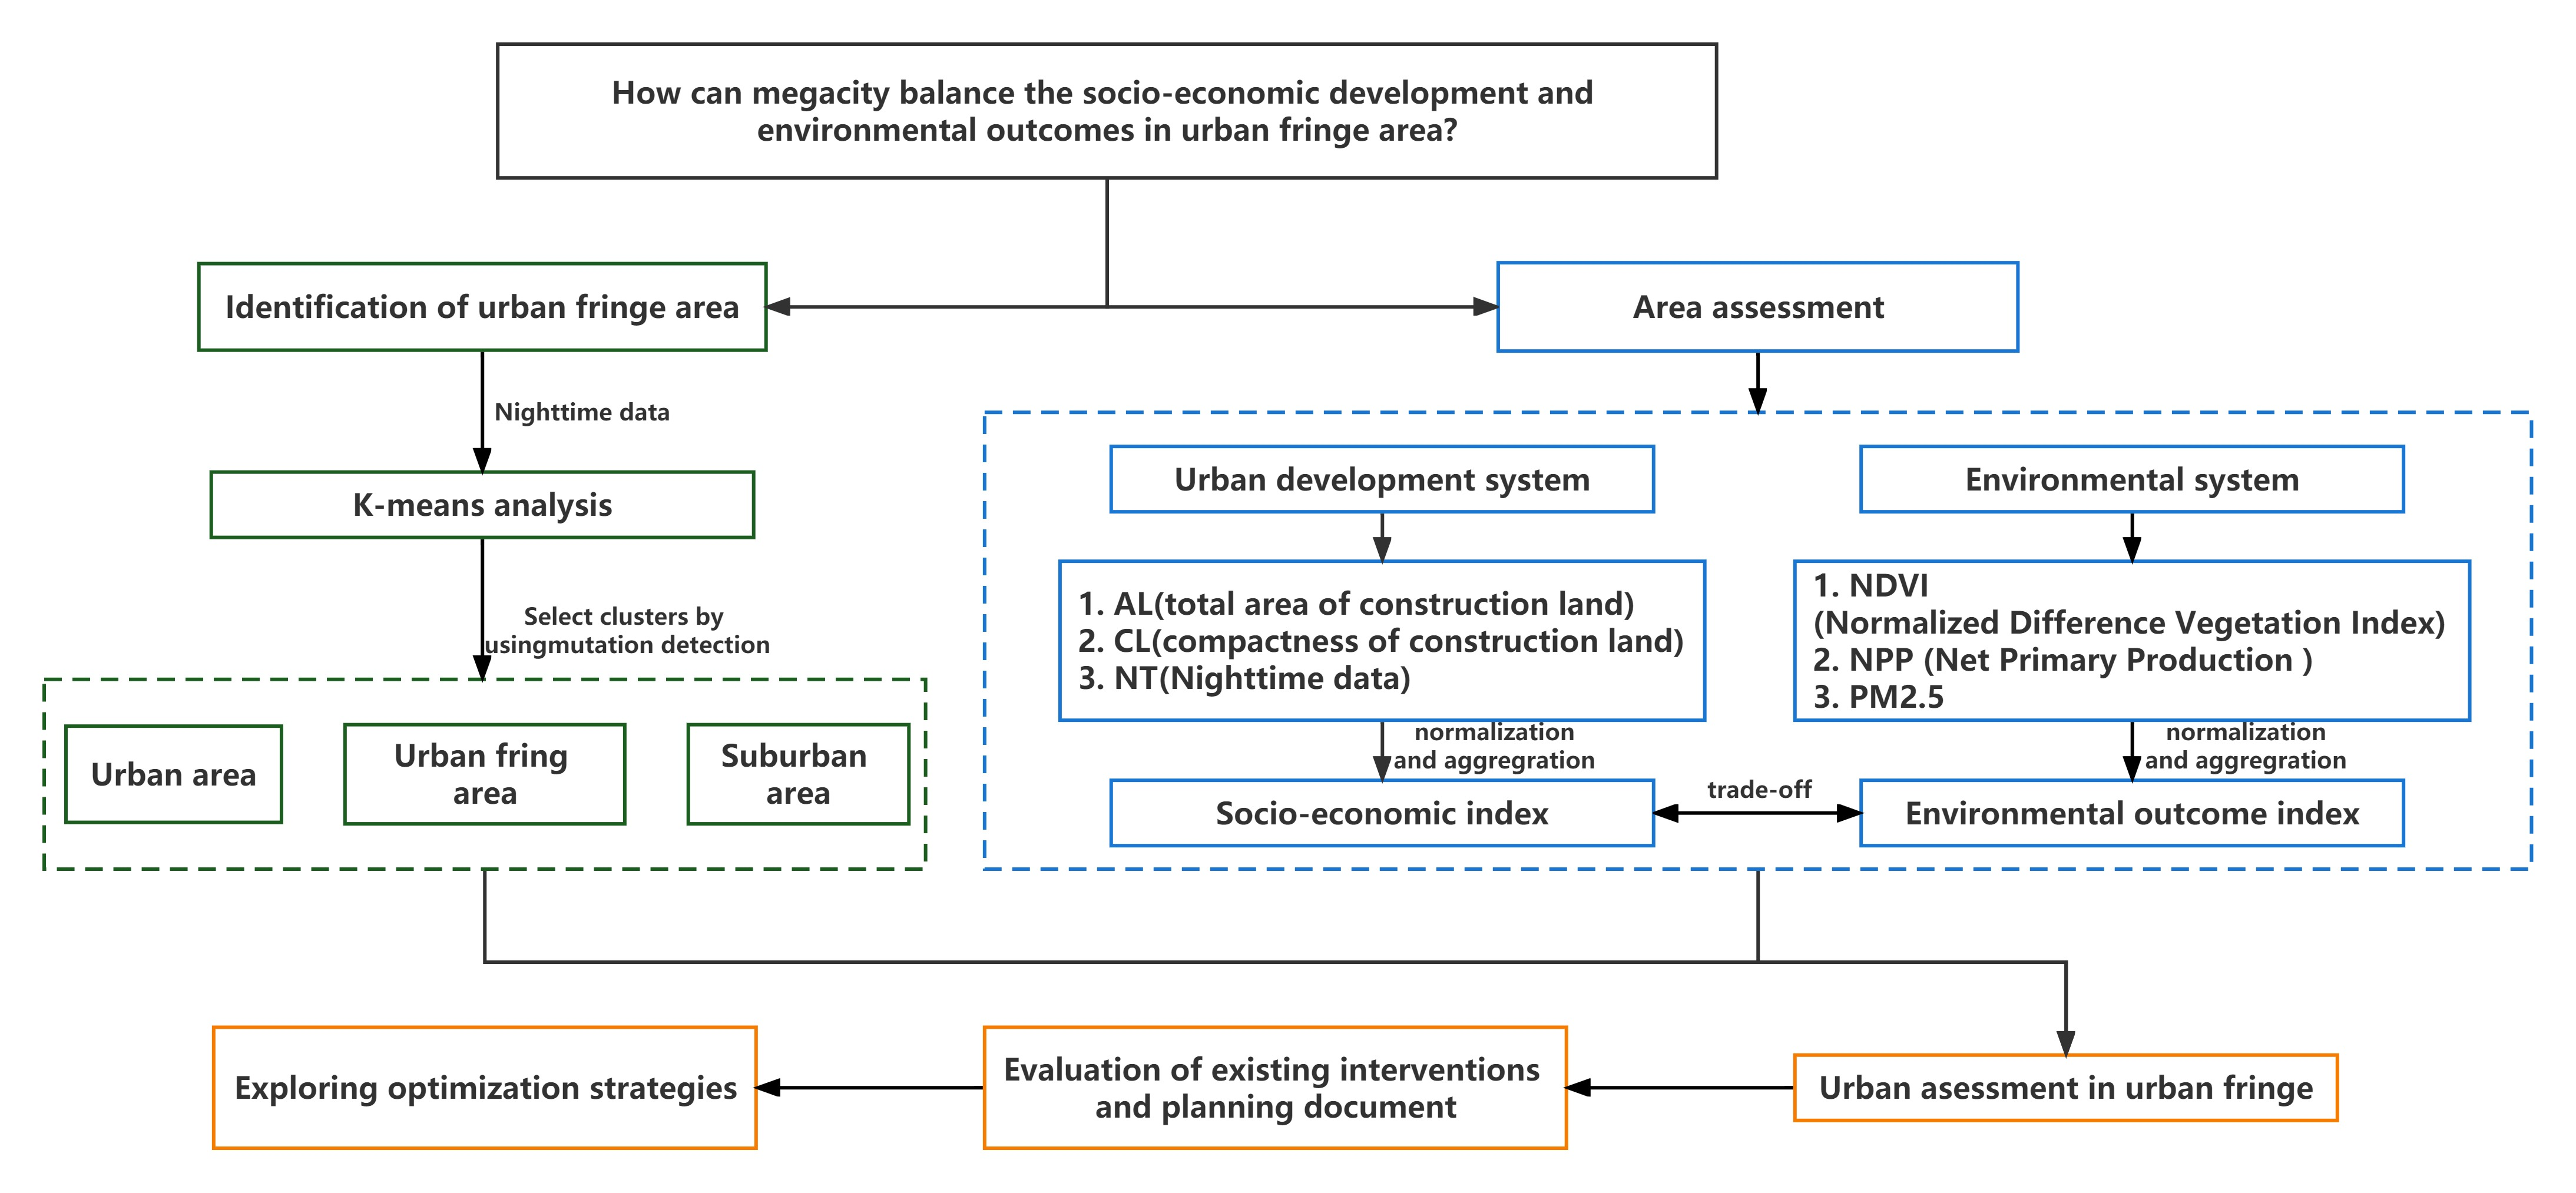
\includegraphics[width=15cm]{Figure/framework0821.jpg}
}
\caption{The framework of the whole study process}
\label{structure}
\end{figure}
%%%%%%%%%%%%%%%%%%%%%%%

\subsection{Ethical Considerations}
The direction of the study was to understand the changing trends and policy orientation of the two systems in urban fringe area through the study of urban development and environmental system. In the context of climate change and urban sprawl, it would provide a sustainable development direction for urban fringe area in megacities.\\

Therefore, all data in this study were studied for the current geographical situation, economic and environmental situation of the area. All data could be publicly available through the Internet. And since the study was designed to analyze the data comprehensively from a larger perspective, the study wouldn't identify or reveal anything about the private lives and habits of individuals. In addition, the analysis results would be based on rigorous data analysis and provide reasonable conclusions and recommendations.\\


\subsection{Study area}

As the top cities in China for economic development, Guangzhou and Shanghai have relied on their coastal advantages to develop their urbanization in the last 30 years. While acting as the core of the metropolitan area, Guangzhou and Shanghai have been under great pressure on ecological space due to their rapid urbanization. Therefore, these cities would be used as case study cities in the study since both of them have similar economic status, geographic location and environment.\\

\subsubsection{Guangzhou}
As the central city in the Guangdong-Hong Kong-Macao Greater Bay Area, Guangzhou (Figure \ref{lulc}a) has a total area of 7434.4 km2. There would be a topographical structure of densely forested mountains in the northern area, which would act as the ecological support area of the whole city. Having the topography of hilly and basins, the central area of Guangzhou would be the socio-economic center. What’s more, with most proportion area of farmland, the southern area is now facing the situation of the urbanization process. Due to its special characteristics as a coastal port near the South China Sea, construction land in the southern area has expanded rapidly and there has been a huge population growth in about 500,000 when it comes to the total area. Therefore, Guangzhou would be one of the cities with urban sprawl problems between socio-economic system and environmental system in the Greater Bay Area \parencite{li_research_2021}.\\

\subsubsection{Shanghai}
Located in Yangtze River estuary, Shanghai (Figure \ref{lulc}b) is the economic center of China, with a permanent population of 7.16 million The total area of Shanghai metropolitan area is 6340.5km2 and it is near the South China. Surrounded by the land use type of farmland and forest, the central area is mainly construction land and the landscape type could be relatively simple. Besides, national natural habitats in Shanghai could prove high ecological value in ecosystem services \parencite{bing_spatial_2021}.\\
%%%%%%%%%%%%%%%%%%%%%%%%%%%%%%%%%%%%
\begin{figure}[h]
\centering
\subfigure[Guangzhou]{
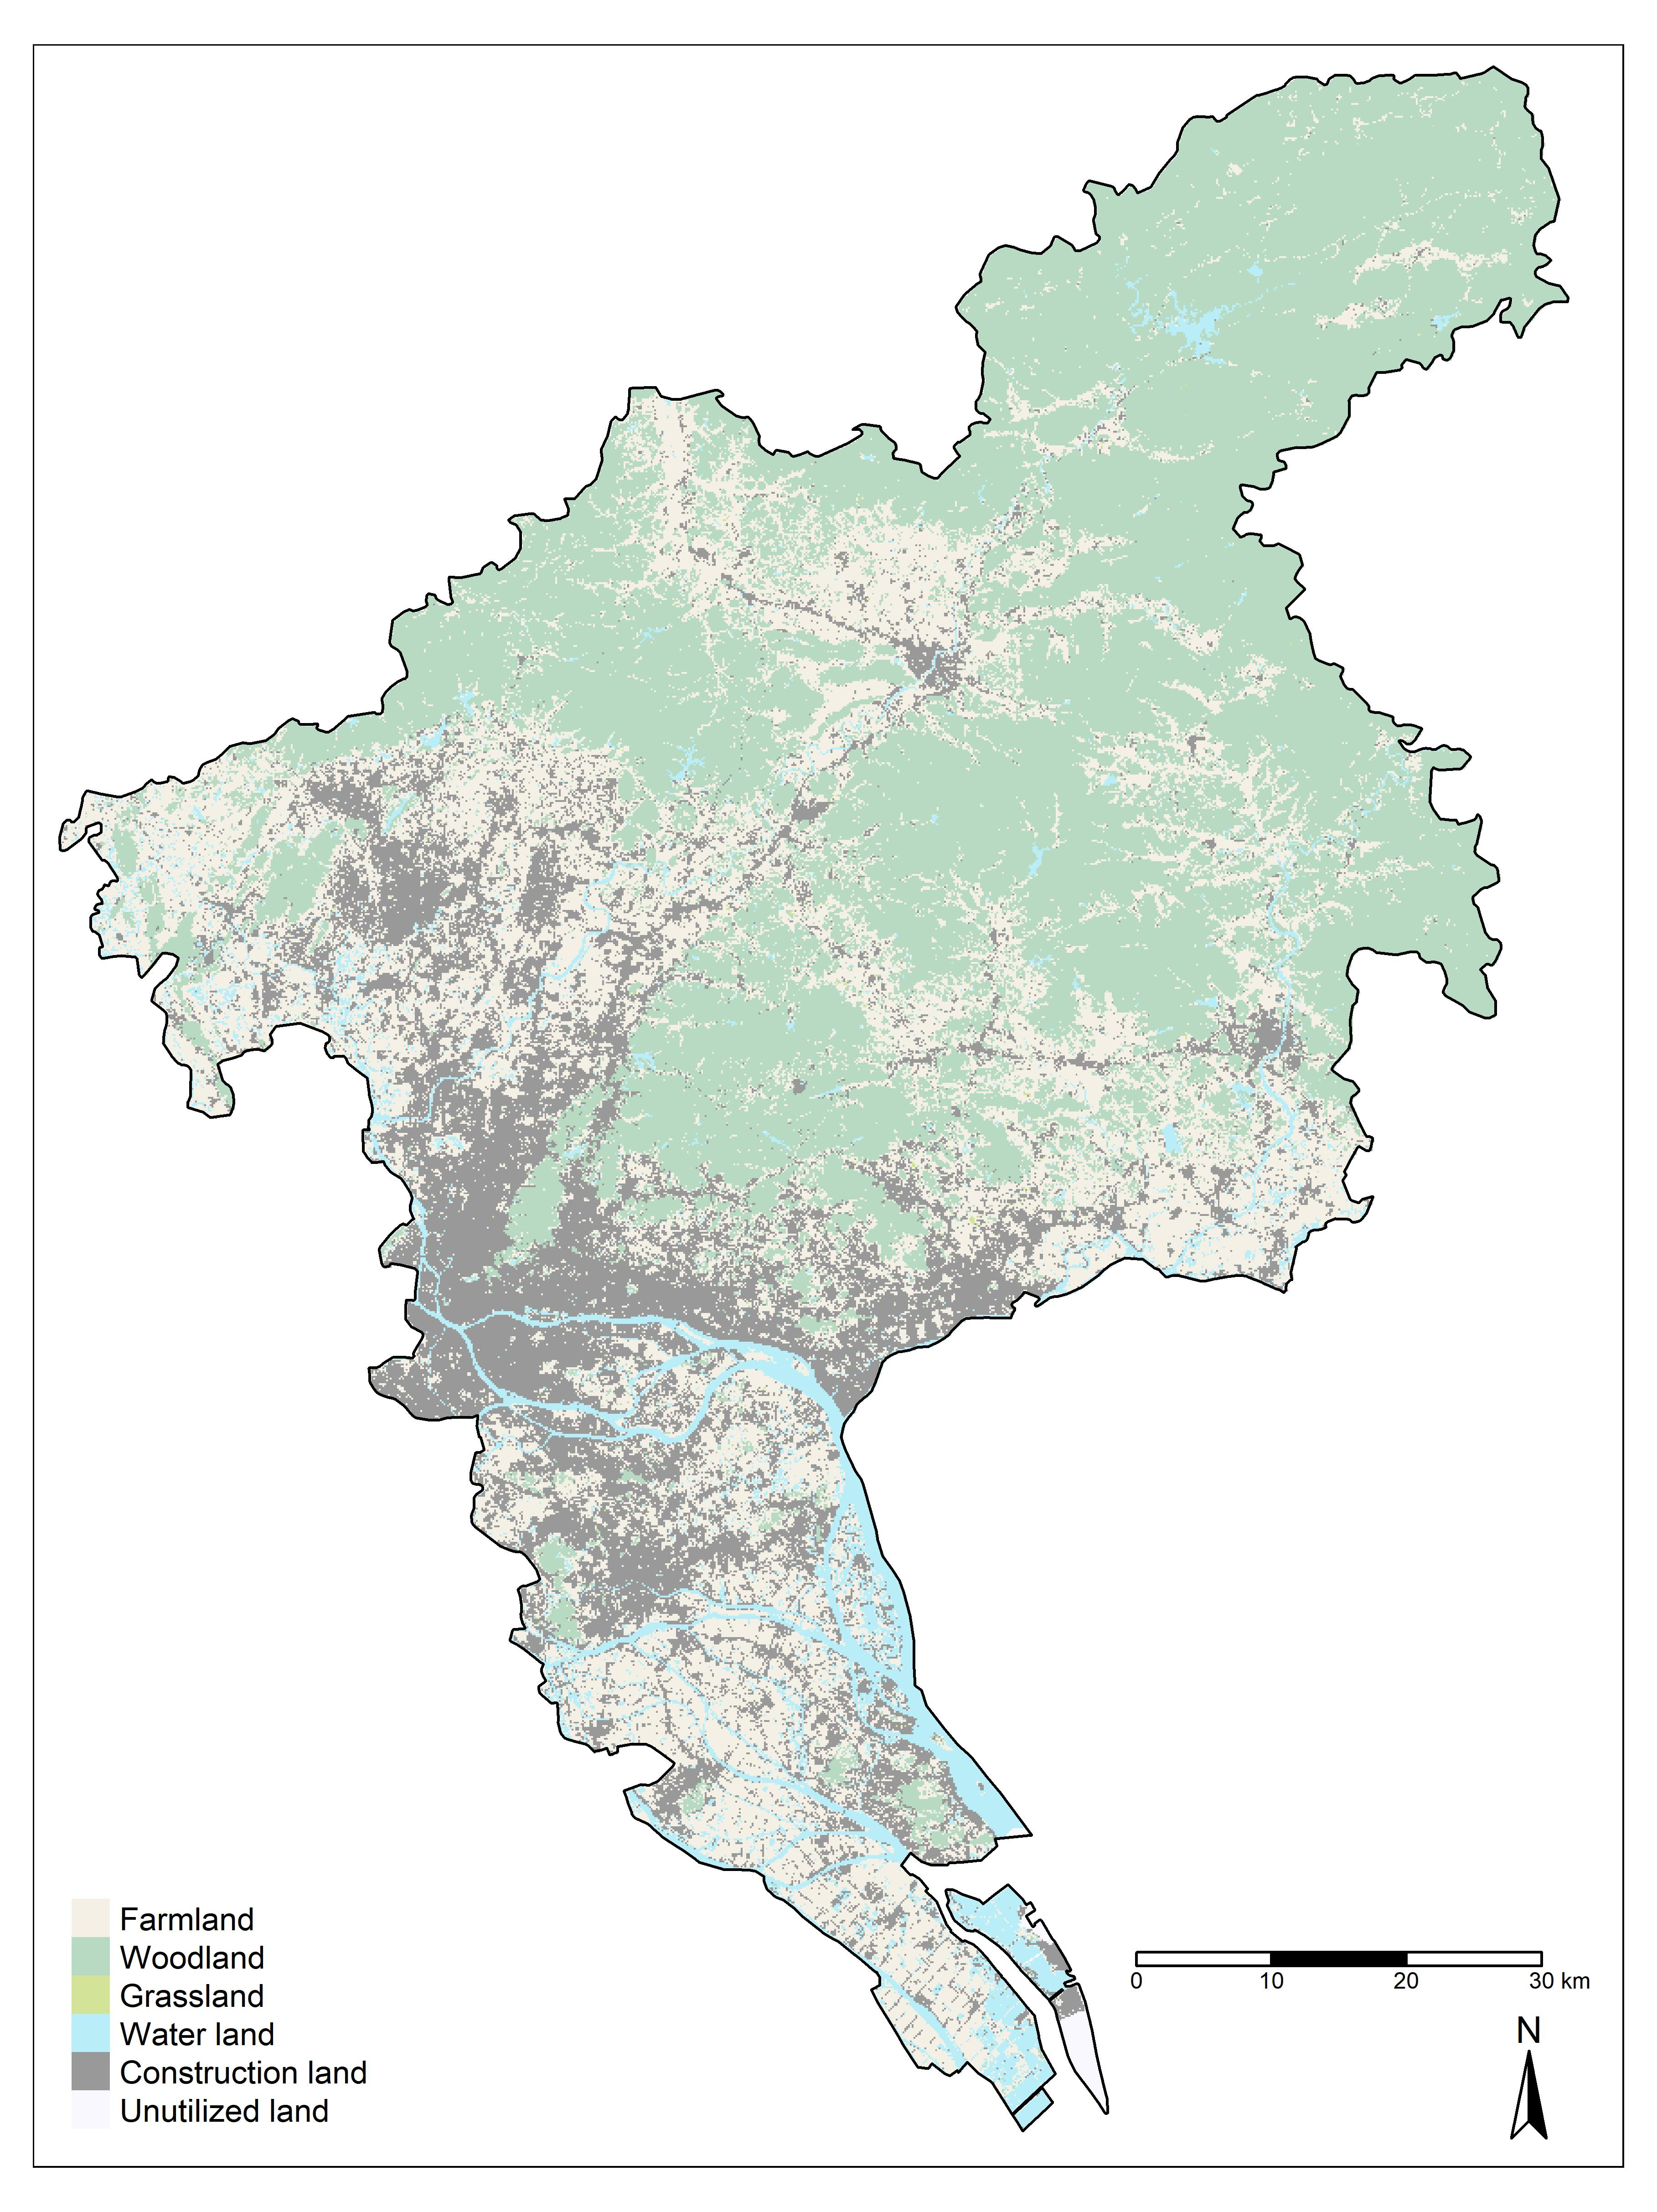
\includegraphics[width=6cm]{Figure/lulcgz.jpg}
}
\quad
\subfigure[Shanghai]{
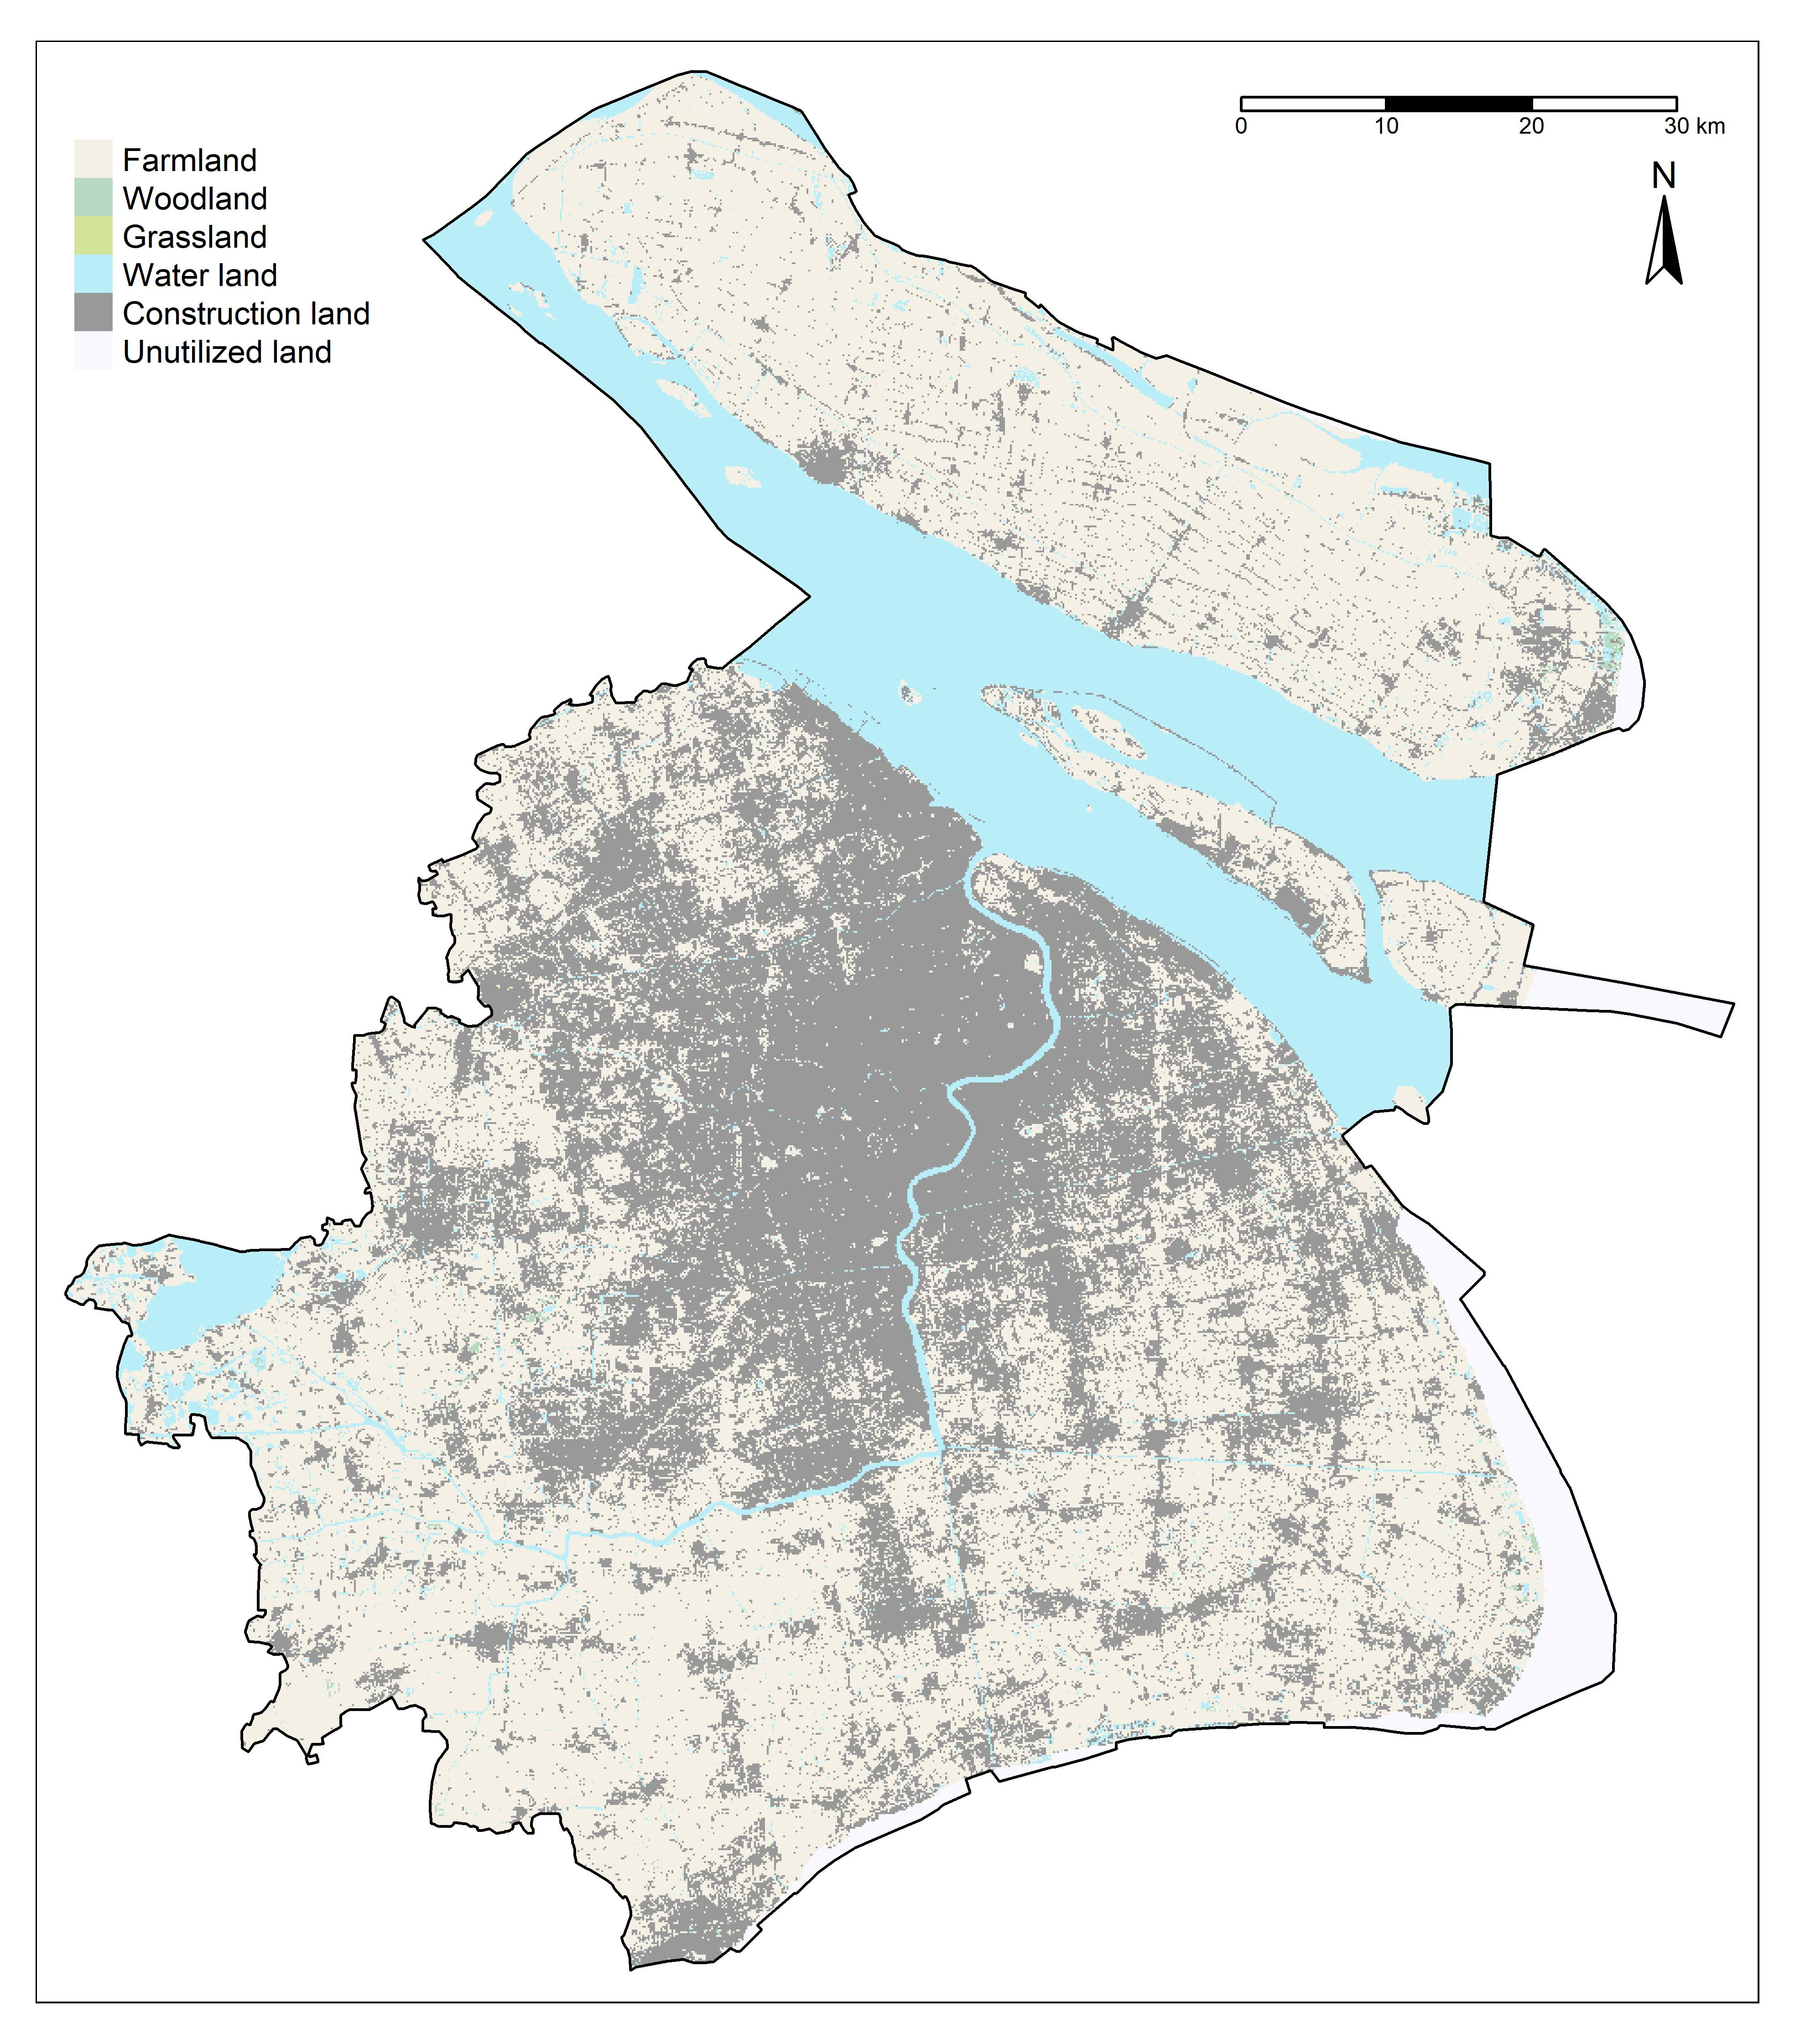
\includegraphics[width=7cm]{Figure/lulcsh.jpg}
}
\caption{Land use land cover of two case study cities}
\label{lulc}
\end{figure}
%%%%%%%%%%%%%%%%%%%%%%%%%%%%%%%%%%%%
\subsection{Dataset}
As this study requires data collection and analysis from the perspective of urban system and environmental system, the following data will be obtained and applied to the actual study.\\

\subsubsection{NDVI}
By using Landsat images on Google Earth Engine\href{https://github.com/Jackeytanlor/CASA_Dissertation/blob/main/code/GEE_NDVI.md}{(GEE)} remote sensing cloud computing platform, The 30m annual NDVI maximum dataset was used from 2013, 2016 and 2019. The NDVI data was calculated by using Landsat 8 remote sensing images from the US Landsat satellite. NDVI maximum for the research area was extracted from each month and generated the annual maximum data in each year. In Landsat 8, NDVI was calculated by using B5 and B4 bands.\\

\subsubsection{Net Primary Production (NPP)}
The global product MODIS (MOD17A3H V0006) Terra time series Net Primary Production (NPP)  at 500m spatial resolution and yearly compositing period was used from 2013, 2016 and 2019. The data source for this product was acquired through the United States Geological Survey (USGS) Land Process, and the data is merged and intercepted by \href{https://github.com/Jackeytanlor/CASA_Dissertation/blob/main/code/GEE_NDVI.md}{GEE} to produce data for the target area.\\

\subsubsection{PM2.5}
By using artificial intelligence and considering the spatio-temporal heterogeneity of air pollution, PM2.5 from The China High Air Pollutants \href{https://weijing-rs.github.io/product.html}{(CHAP)} dataset was used from 2013, 2016 and 2019. The data source for this product, ground-level air pollution in China, could have long-term, full-coverage, high-resolution and high quality \parencite{wei_chinahighpm10_2021}. The dataset was acquired through open access link, and the data was merged and intercepted by R to extract data for the target area.\\

\subsubsection{Land use land cover (LULC)}
By using Landsat images on GEE, Landsat-derived annual land cover product of China (CLCD) from 2013, 2016 and 2019. In order to improve the spatial-temporal consistency of LULC compared with Landsat dataset, the dataset used a post-processing method, which may include spatial-temporal filtering and logical reasoning \parencite{yang_30_2021}. The dataset is acquired through \href{https://doi.org/10.5281/zenodo.4417810}{Zenodo} (\url{https://doi.org/10.5281/zenodo.4417810}).\\

\subsubsection{Nighttime data (NT)}
The global Nighttime data Suomi-NPP VIIRS-derived nighttime lights at 500m spatial resolution and yearly compositing period was used from 2013, 2016 and 2019. The data source for this product was acquired through National Oceanic and Atmospheric Administration \href{https://github.com/Jackeytanlor/CASA_Dissertation/tree/main/dataset/NT}{(NOAA)}.\\

\subsection{Methods}
\subsubsection{Identification of urban fringe area}
\subsubsubsection{Fluctuation theory}
Due to production and lifestyle differences, citizens from urban area are more likely to use light at night and it would be much more than those who live in suburban area. From urban area to urban fringe and suburban area, nighttime lighting tensity would change to decrease followed by the gradual decrease of urbanization development level. On the other hand, the NT value within urban area and suburban area will be in a flat state because the land use type is relatively single and has not been affected in a short period of time. However, Due to the excessive impact of being in the city center to the countryside in urban fringe area, there might be more complex in land use type, which would show the characteristic of shows characteristics of transition, diversity, and fluctuation. The area will be influenced by urbanization in a short period of time, so the NT value in the area will be in a fluctuating state. Therefore, NT value will show a 'smooth-fluctuating-smooth' characteristic as the surrounding environment changes from urban area to urban fringe and suburban area. Based on the existing NT value change characteristics, a combined–value method was used to identify urban fringe area \parencite{yang_spatial_2017}.\\

According to the combined-value method, cluster analysis would be used in the identification of urban fringe area. When it comes to the selection of cluster analysis methods, the K-means analysis would be a popular method for identifying urban areas. Although the cluster method of K-means may have a shortage of low sensitivity to initial points because of its clear clustering structure and simple clustering process. The method would be not only easy to use but also avoids the errors from clustering methods such as DBSCN due to land use dispersion \parencite{feng_using_2020}.\\

By using a given number of clusters n and dataset containing different dimensions of data objects as input, K-means analysis can comprehensively compare the attributes and values of different data objects. Finally, the model would output object with the highest similarity in the same cluster.\\

\subsubsubsection{Nighttime light and Light Fluctuation}
According to the combined–value method, 2 dimensions of the data objects would be introduced in the K-means analysis. NT value would be one aspect of the data object, since it can show the light intensity, which can show the difference between central area and the non-central area. However, the accuracy of the data may not be as accurate as in a developed country, which may result in a small amount of error \parencite{zhang_can_2013}.\\

Light fluctuation would be the second data object. The degree of fluctuation of light intensity would help to explore the degree of variation of the light intensity in a certain range, which can do help to find the urban fringe area. Therefore, the study used two indicators, nighttime index and nighttime fluctuation, to perform a cluster analysis of the area, which allows for a more accurate identification of the area in two dimensions.\\

\subsubsubsection{Calculation of light fluctuation}
The calculation of the degree of fluctuation of light intensity(DF) would be shown as below:\\

\begin{equation}
DF=NT_{max}-NT_{min}
\end{equation}

Where DF is the degree of fluctuation. $NT_{max}$ and $NT_{min}$ would be the maximum and minimum value of nighttime light intensity.\\

According to the relevant research, in order to calculate the DF value, $NT_{max}$ and $NT_{min}$ should be selected in the 3*3 neighborhood by using neighborhood analysis \parencite{feng_using_2020}. It can find the exact fluctuation value from the smallest range of raster data.\\

In order to process K-means analysis with these two objects, normalization of the data would be required. Max-Min normalization should be used to standardize the data from 0 to 1. The calculation of normalization would be shown as below:\\

\begin{equation}
NT_{nor}=\frac{NT-NT_{min}}{NT_{max}-NT_{min}}
\end{equation}
\begin{equation}
DF_{nor}=\frac{DF-DF_{min}}{DF_{max}-DF_{min}}
\end{equation}

Where $NT_{nor}$ is the normalization value of nighttime light intensity; $DF_{nor}$ is the normalization value of the degree of fluctuation.\\

\subsubsubsection{Selection of clusters}
Since the K-means analysis in this study needs to explore the clusters of n in the two study area and find the value of n that best matches the study area. Since the research would need to find out 3 kinds of area: urban area, urban fringe area and suburban area, n should be started with 3. Besides, by adjusting the parameter of n, the study can find that the space in the different clusters becomes fragmented as the value of n increases. As the number of clusters rises, so does the complexity of the area \parencite{yang_spatial_2017}. When n \textgreater 10, clusters will intersperse in space, which is not conducive to the application of this study from the study area to other areas. Therefore, a total of 3-10 clusters are presented by the k-means method and the most suitable clusters would be selected by combining the performance of the two urban indicators in the urban fringe area. \\

In the meanwhile, according to research, in order to find the most suitable clusters in case study cities, it is necessary to use mutation detection to observe the result of cluster analysis and compare it with 2 objects. In this study, a straight line is drawn in 2 objects and the line will pass through as many clusters as possible. through this line, a section of the map would be shown and the variation and fluctuation of 2 objects in this section will be shown in the graph (Figure \ref{cluster7}). By comparing the fluctuations of Land use, NT and DF values, the study will select the most suitable n value as the best cluster number.\\

By comparing fringe area identified from the planning document from Guangzhou and Shanghai, 7 clusters are more able to show the mutation values in the area. According to Figure \ref{section}, it could be found that when the section line in Figure \ref{section}ab moves from south to north, the NT and DN values showed fluctuations with the position. It is obvious that some areas showed a significant decrease in DN value when NT value was at the highest point, which could be considered in Cluster n=7(Figure \ref{section}bc) This could demonstrate that the clustering of edge regions could be more clearly identified when there were multiple clusters. Therefore, 7 clusters were used as the final cluster for identification in this study. Therefore, the study may choose n=7 as the result and merge different cluster into 3 area, urban area, urban fringe area and suburban area.\\

%%%%%%%%%%%%%%%%%%%%%%%%%%%%%%%%%%%%
\begin{figure}[h]
\centering
\subfigure[Guangzhou]{
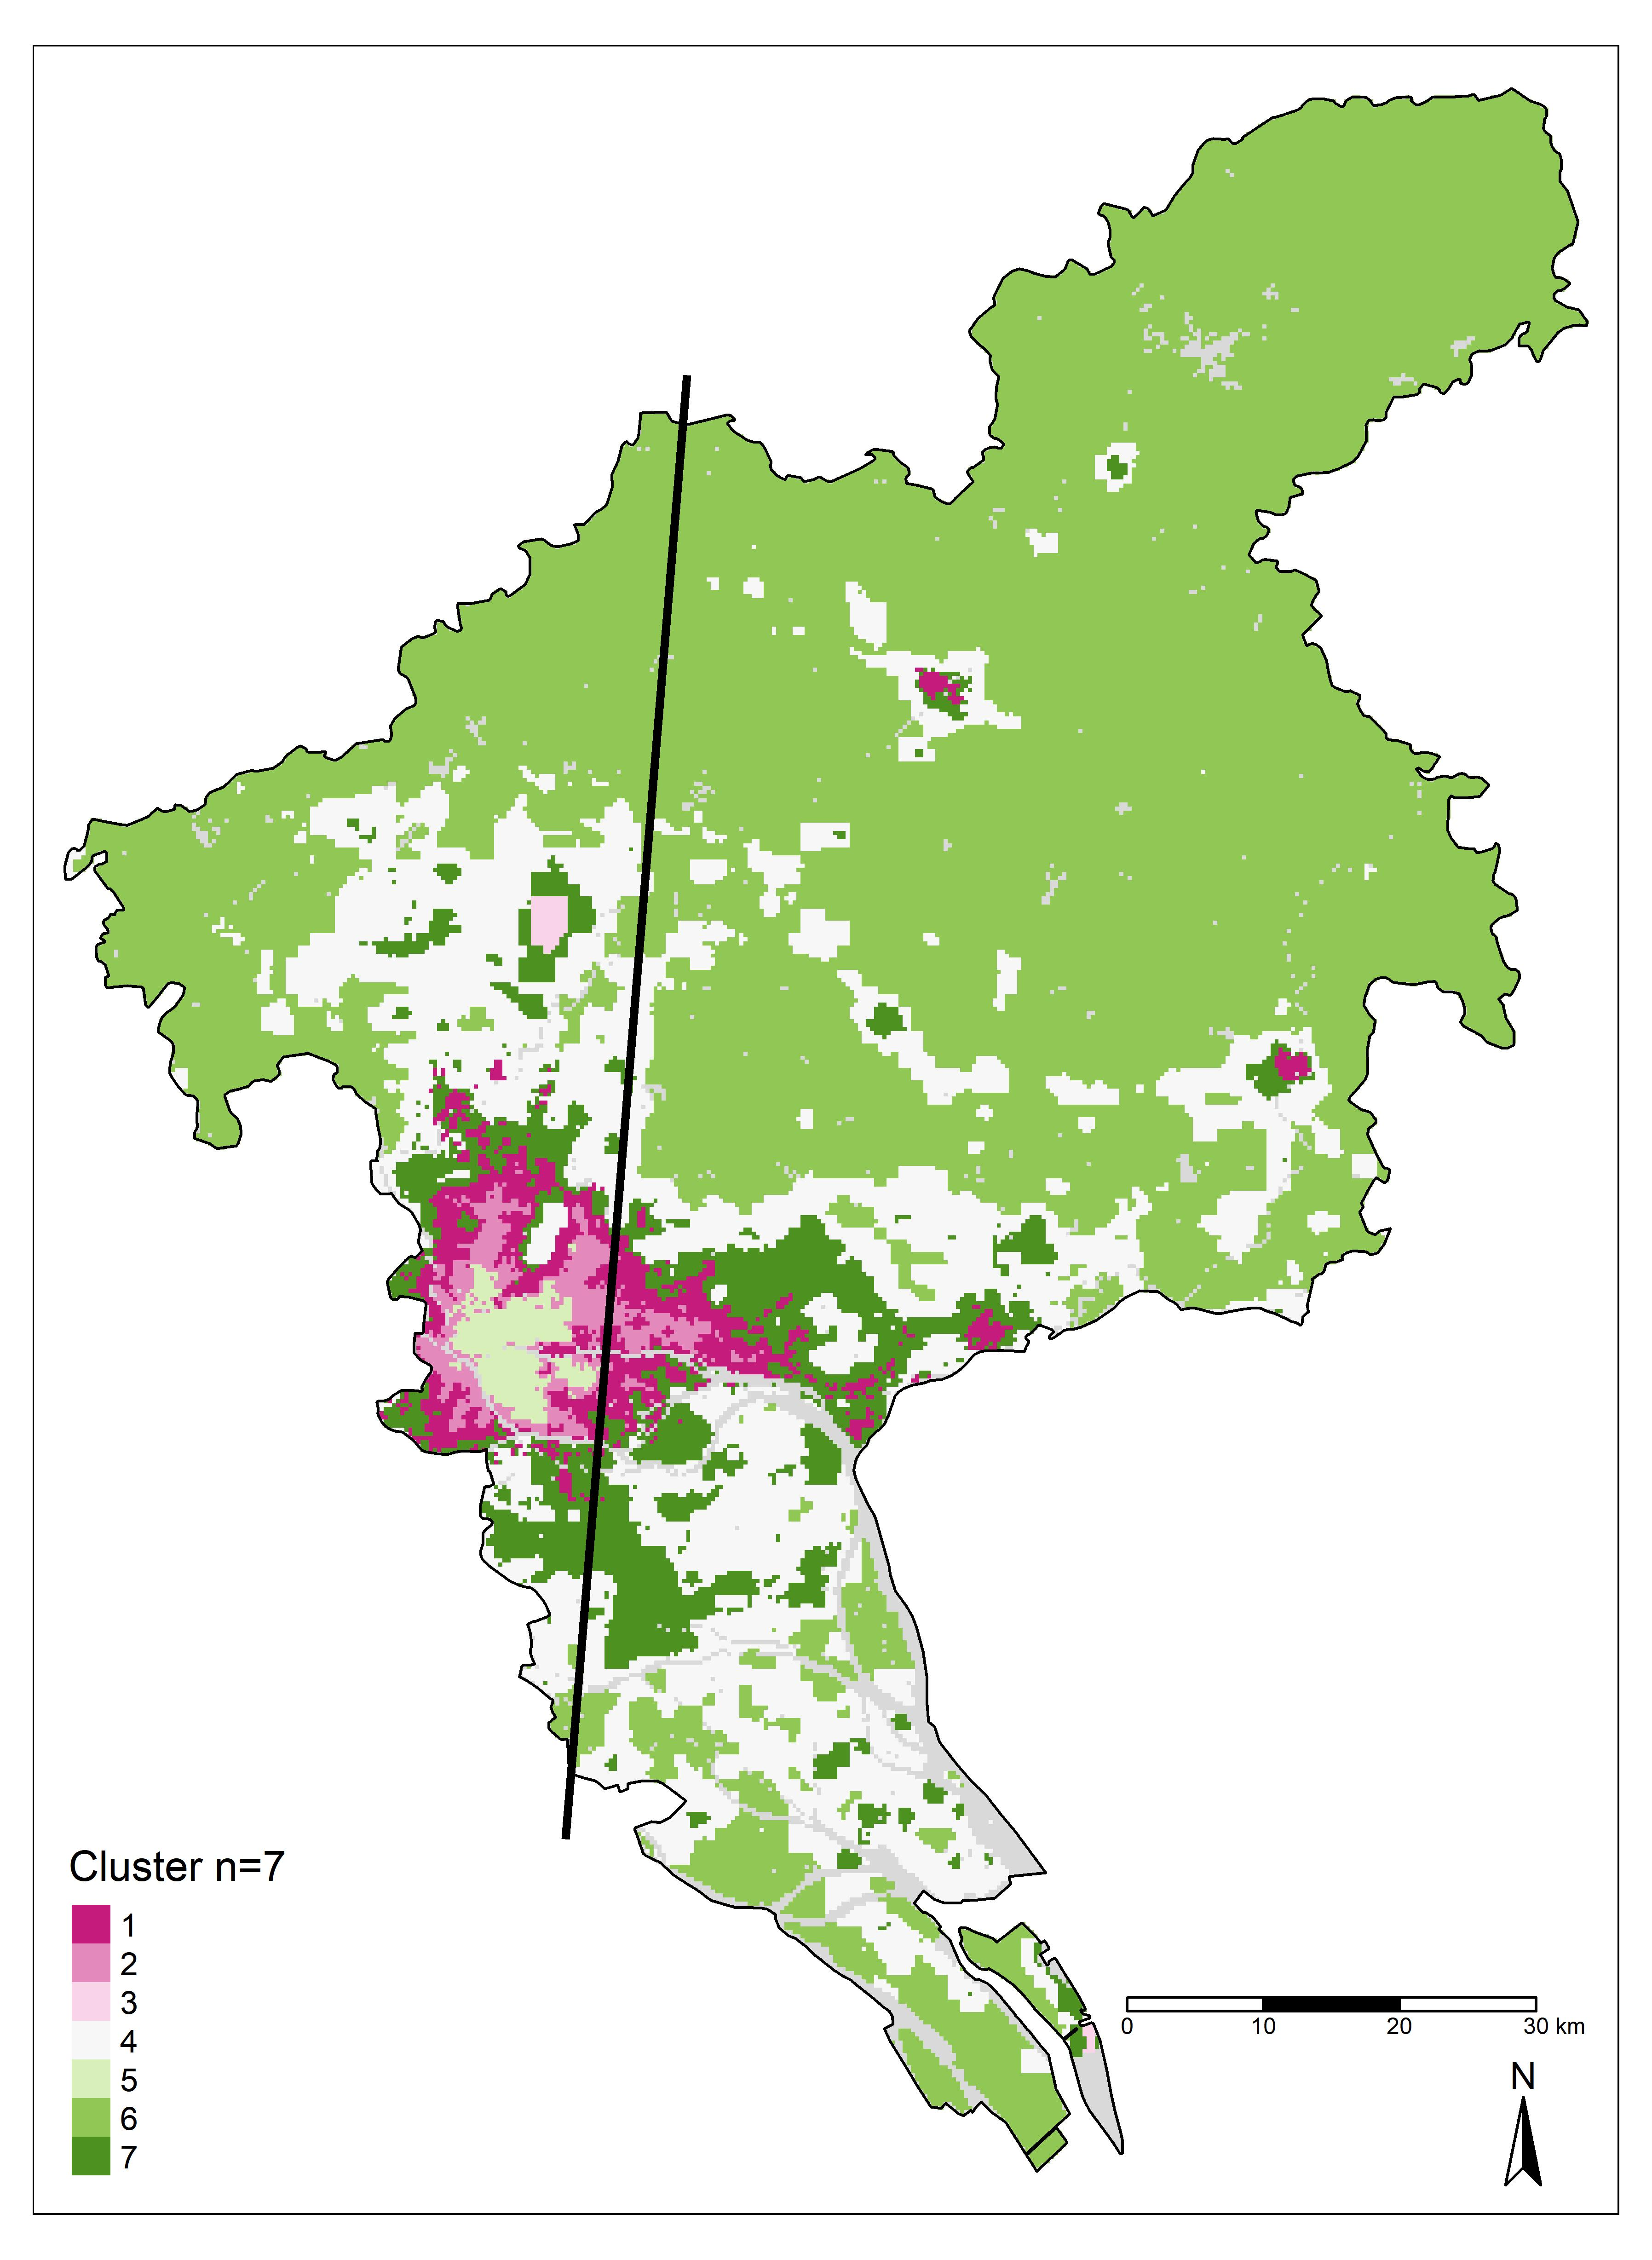
\includegraphics[width=6cm]{Figure/cluster7_0821.jpg}
}
\quad
\subfigure[Shanghai]{
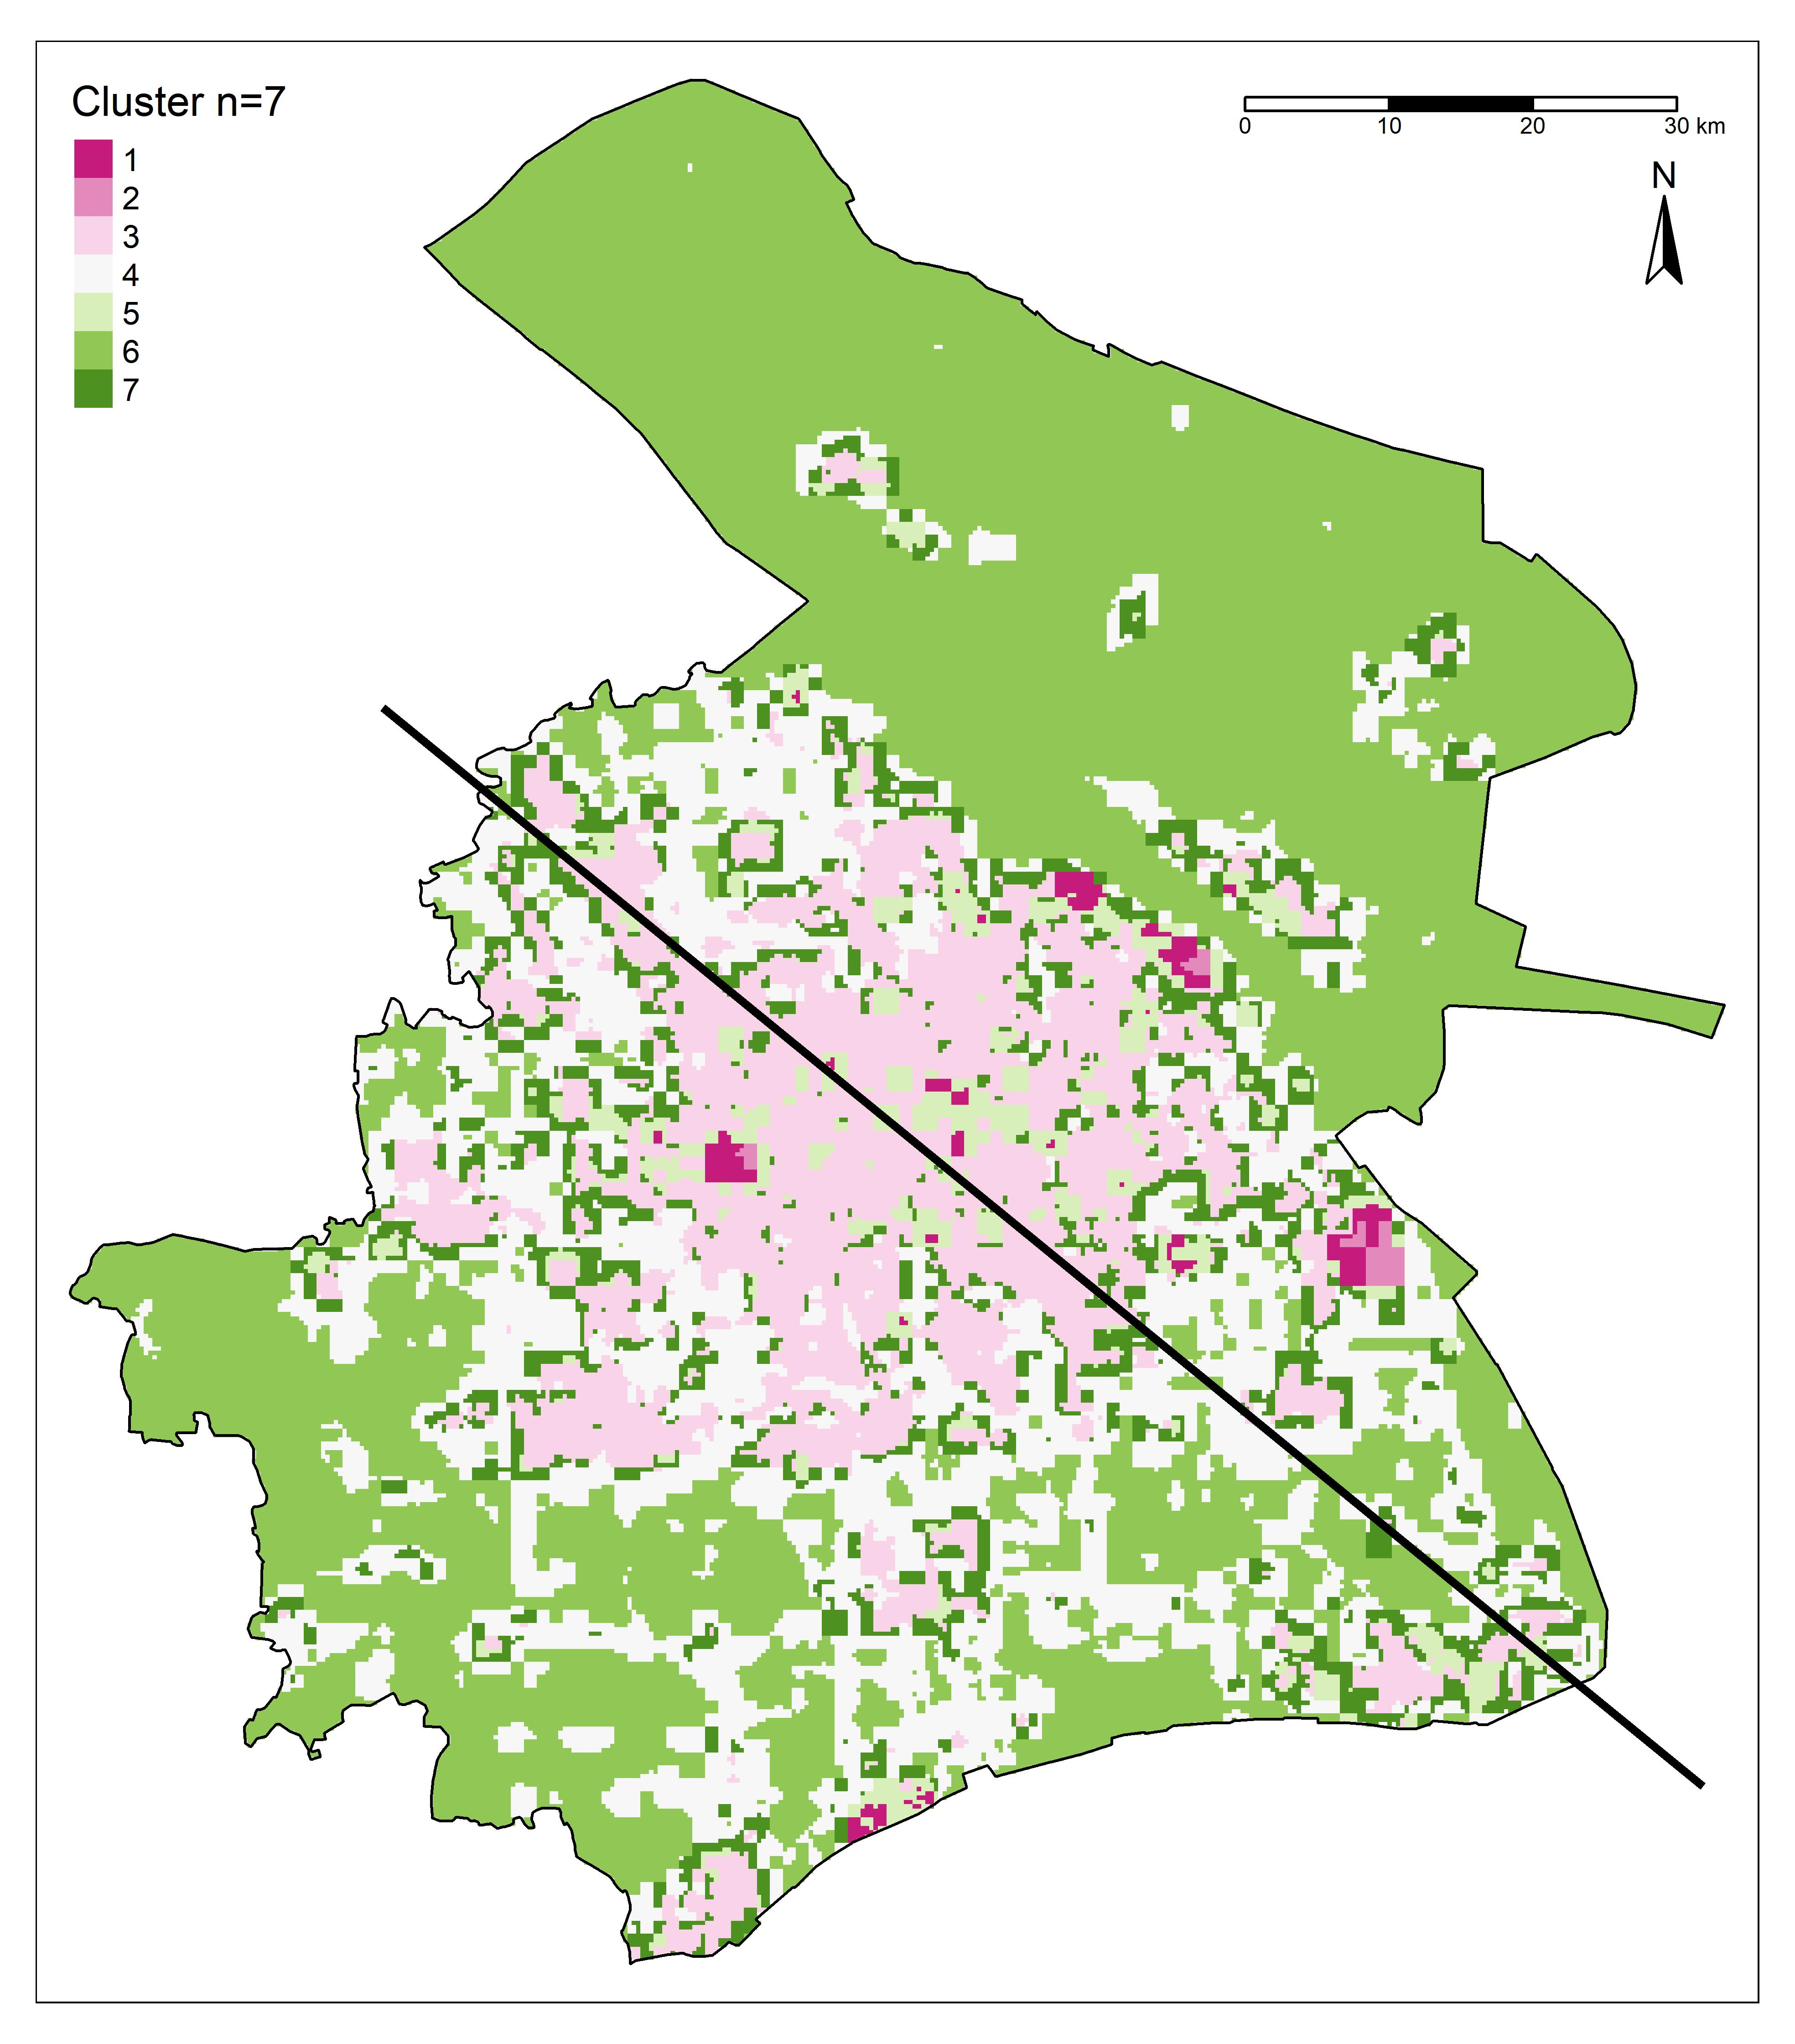
\includegraphics[width=7cm]{Figure/clustersh7_0821.jpg}
}

\caption{The distribution result of clusters (n=7) in the study area with section line}
\label{cluster7}
\end{figure}
%%%%%%%%%%%%%%%%%%%%%%%%%%%%%%%%%%%%

%%%%%%%%%%%%%%%%%%%%%%%%%%%%%%%%%%%%
\begin{figure}[h]
\centering
\subfigure[Guangzhou]{
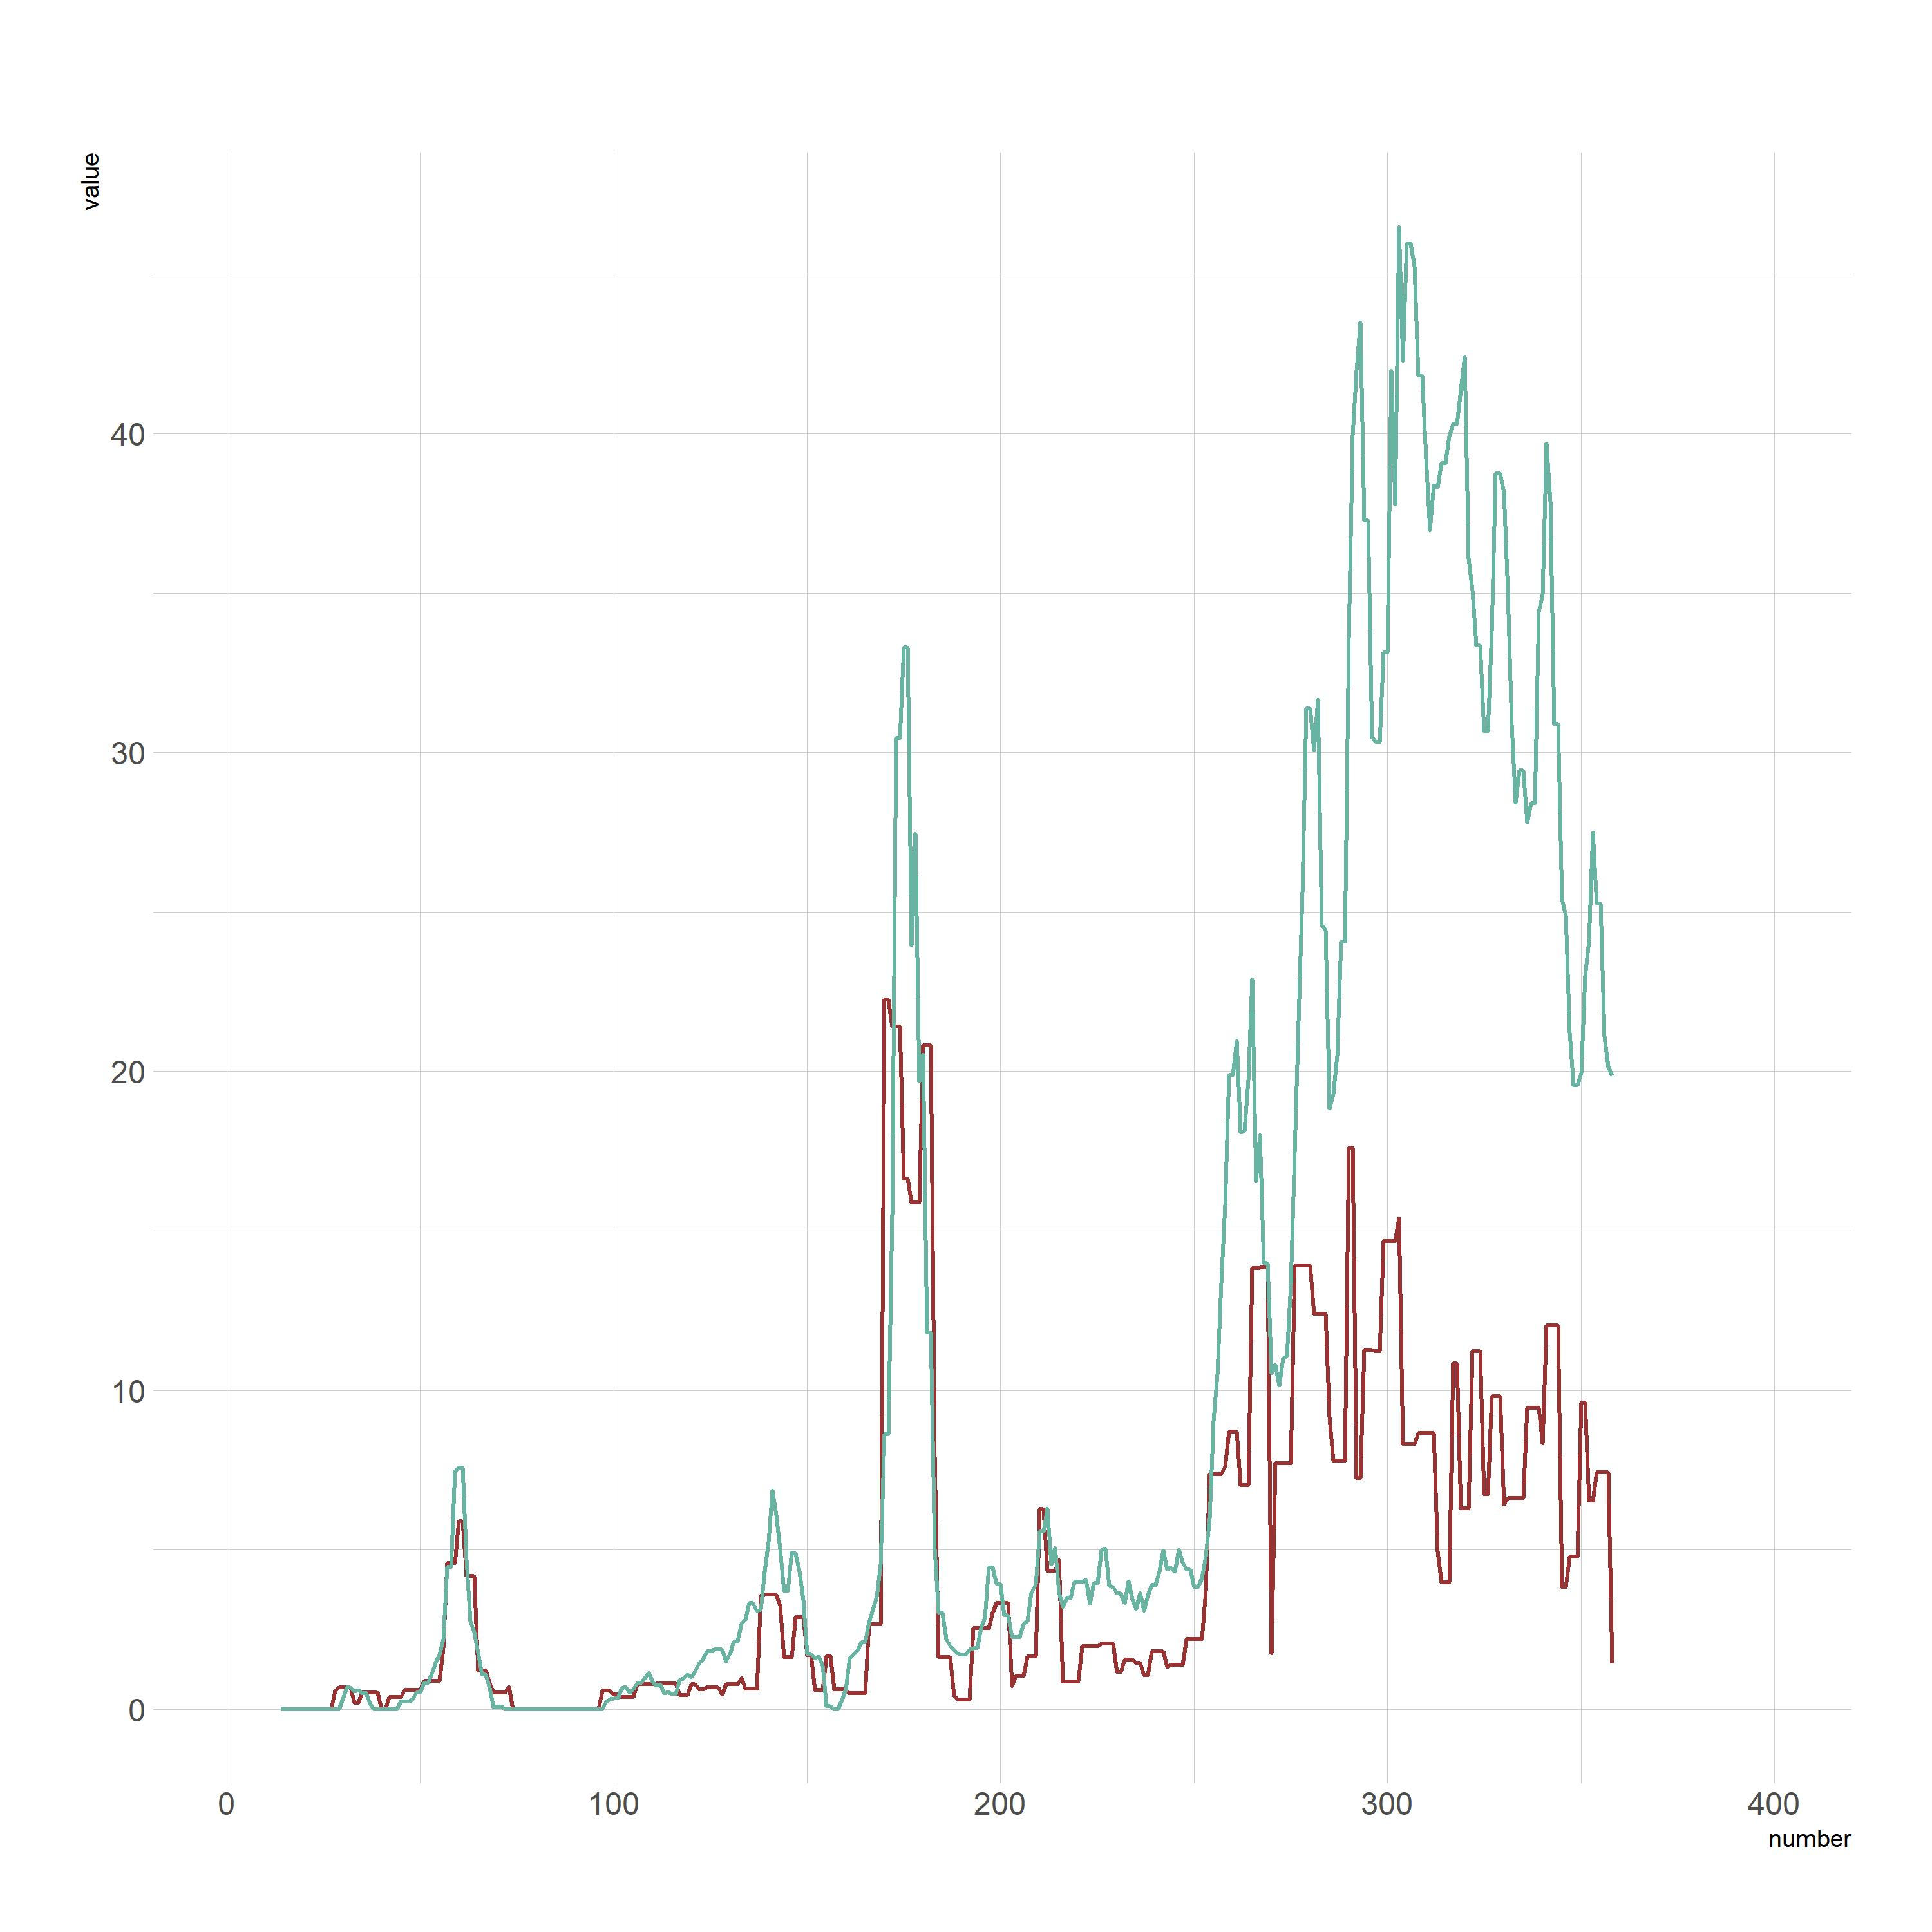
\includegraphics[width=6cm]{Figure/nt0821.jpg}
}
\quad
\subfigure[Shanghai]{
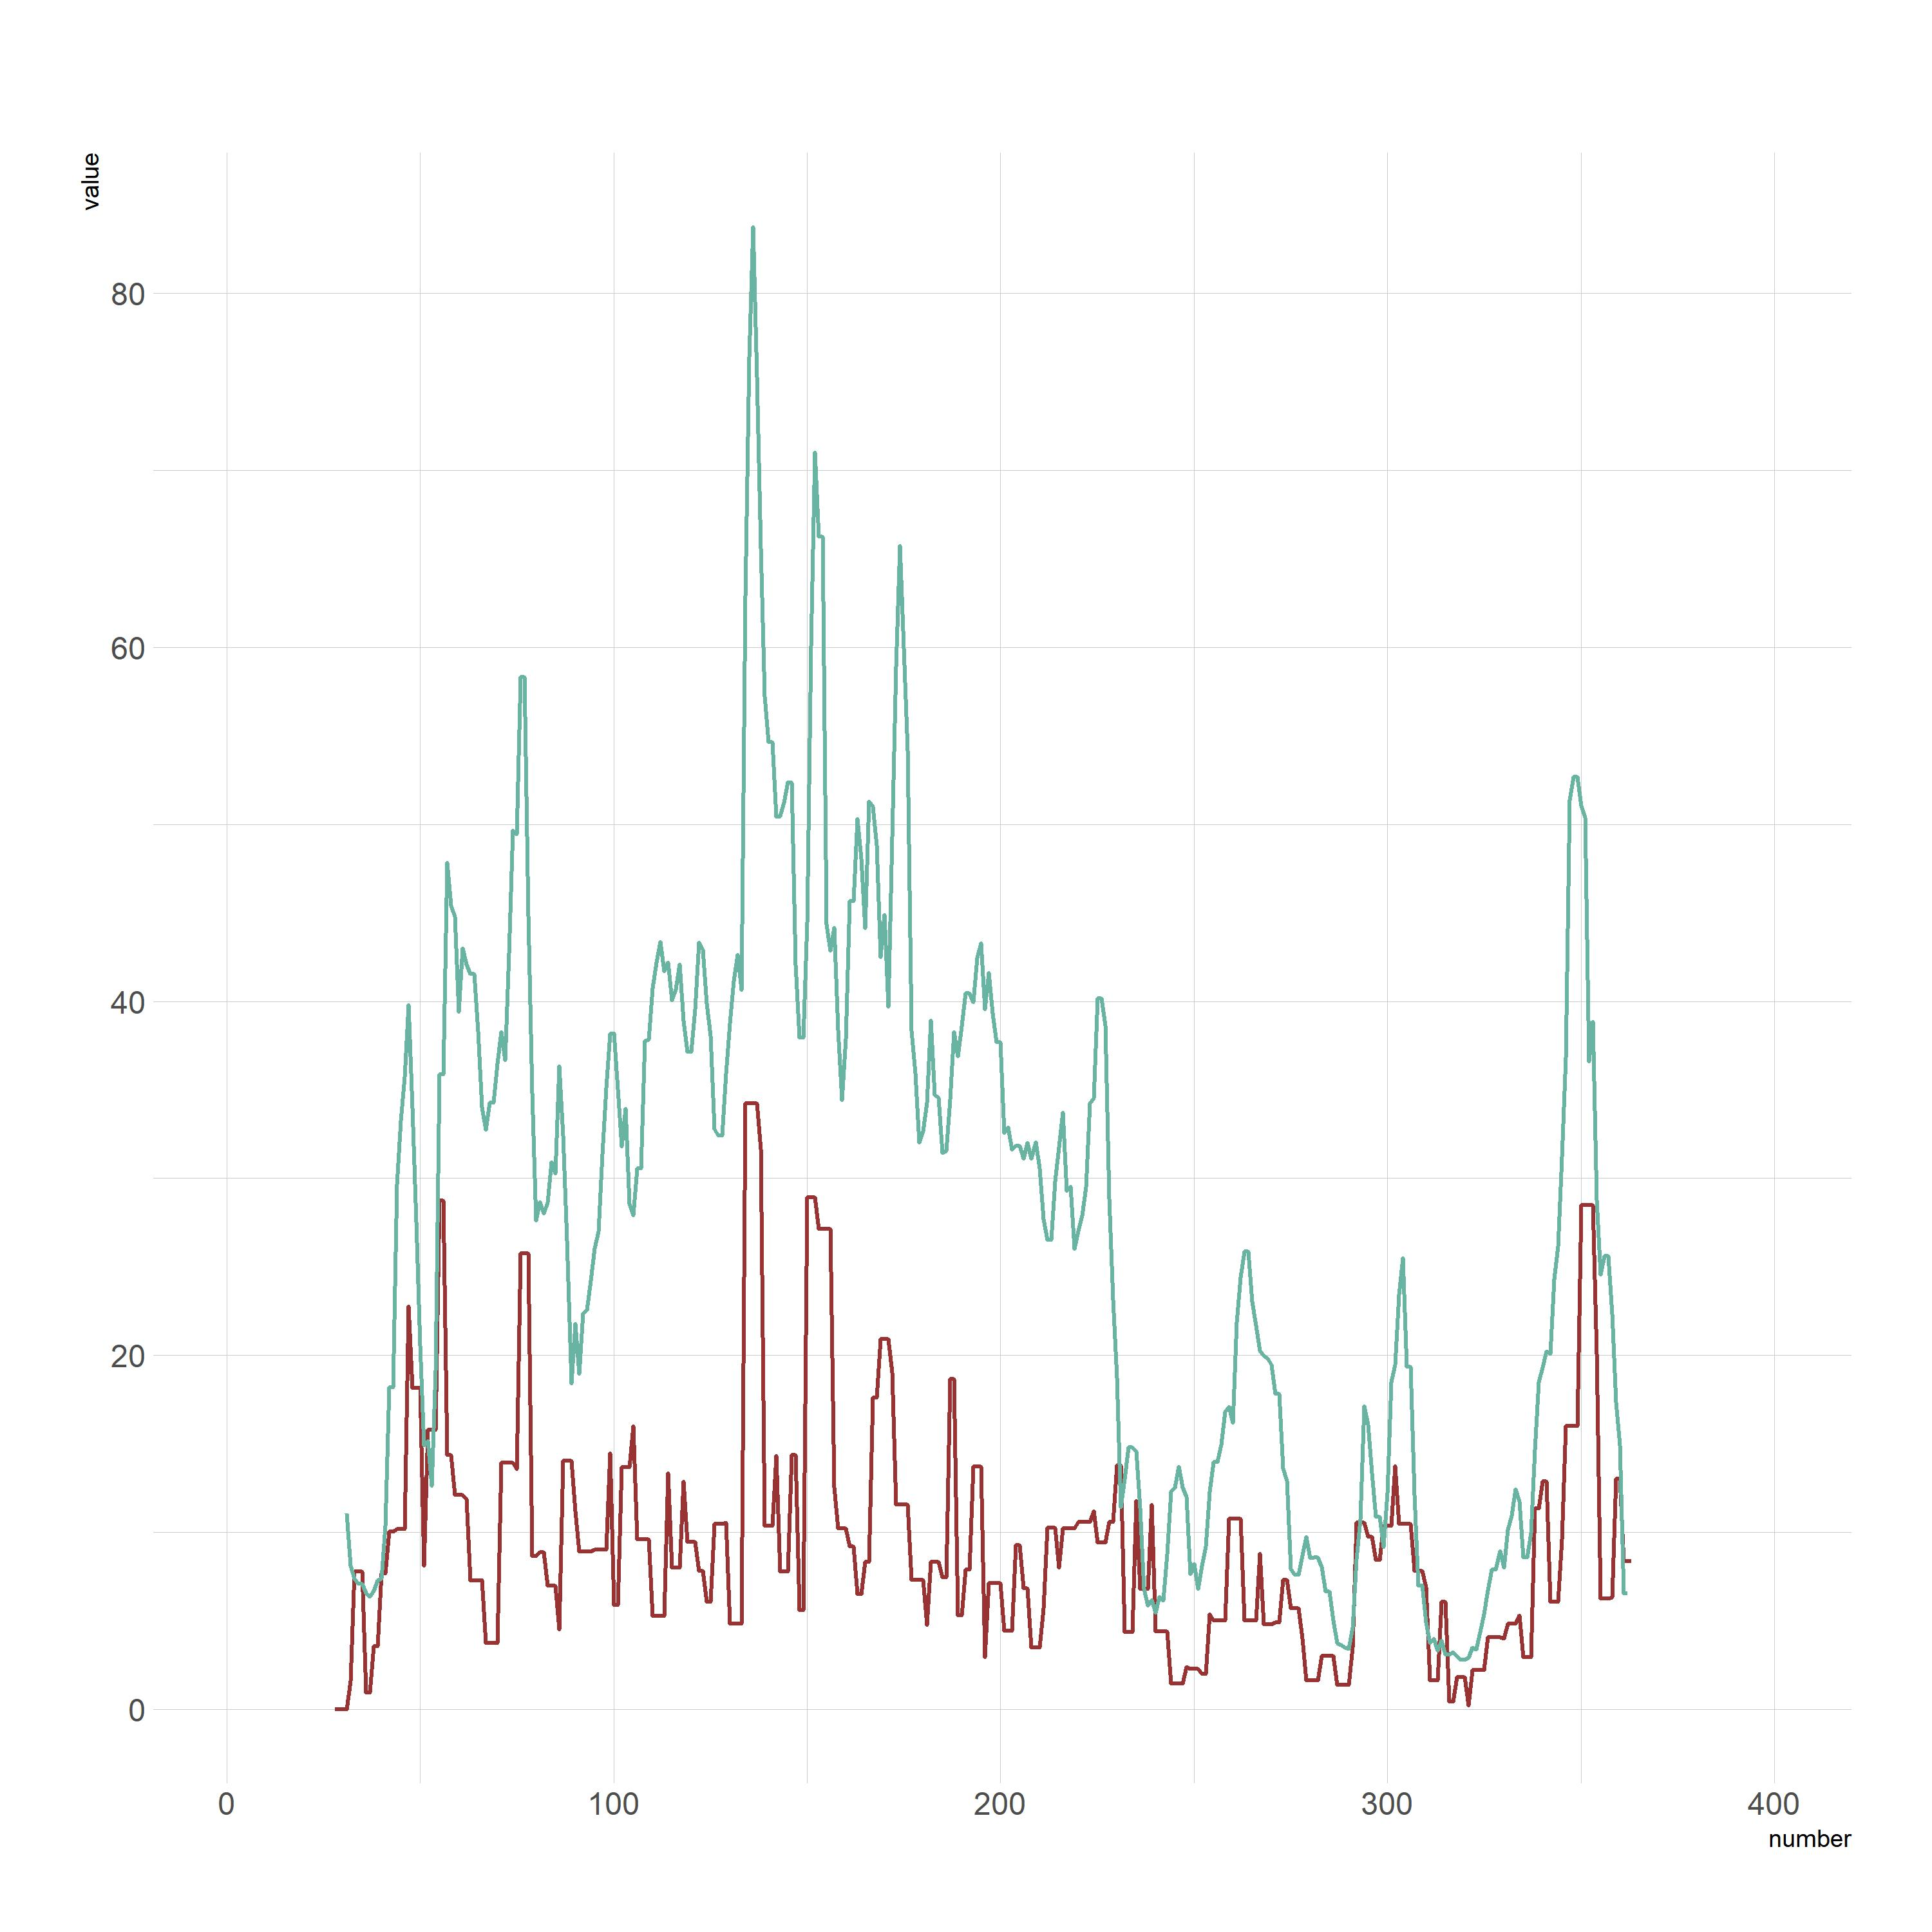
\includegraphics[width=6cm]{Figure/nt_sh0821.jpg}
}
\quad
\subfigure[Performance of section line in cluster n=7(Guangzhou) ]{
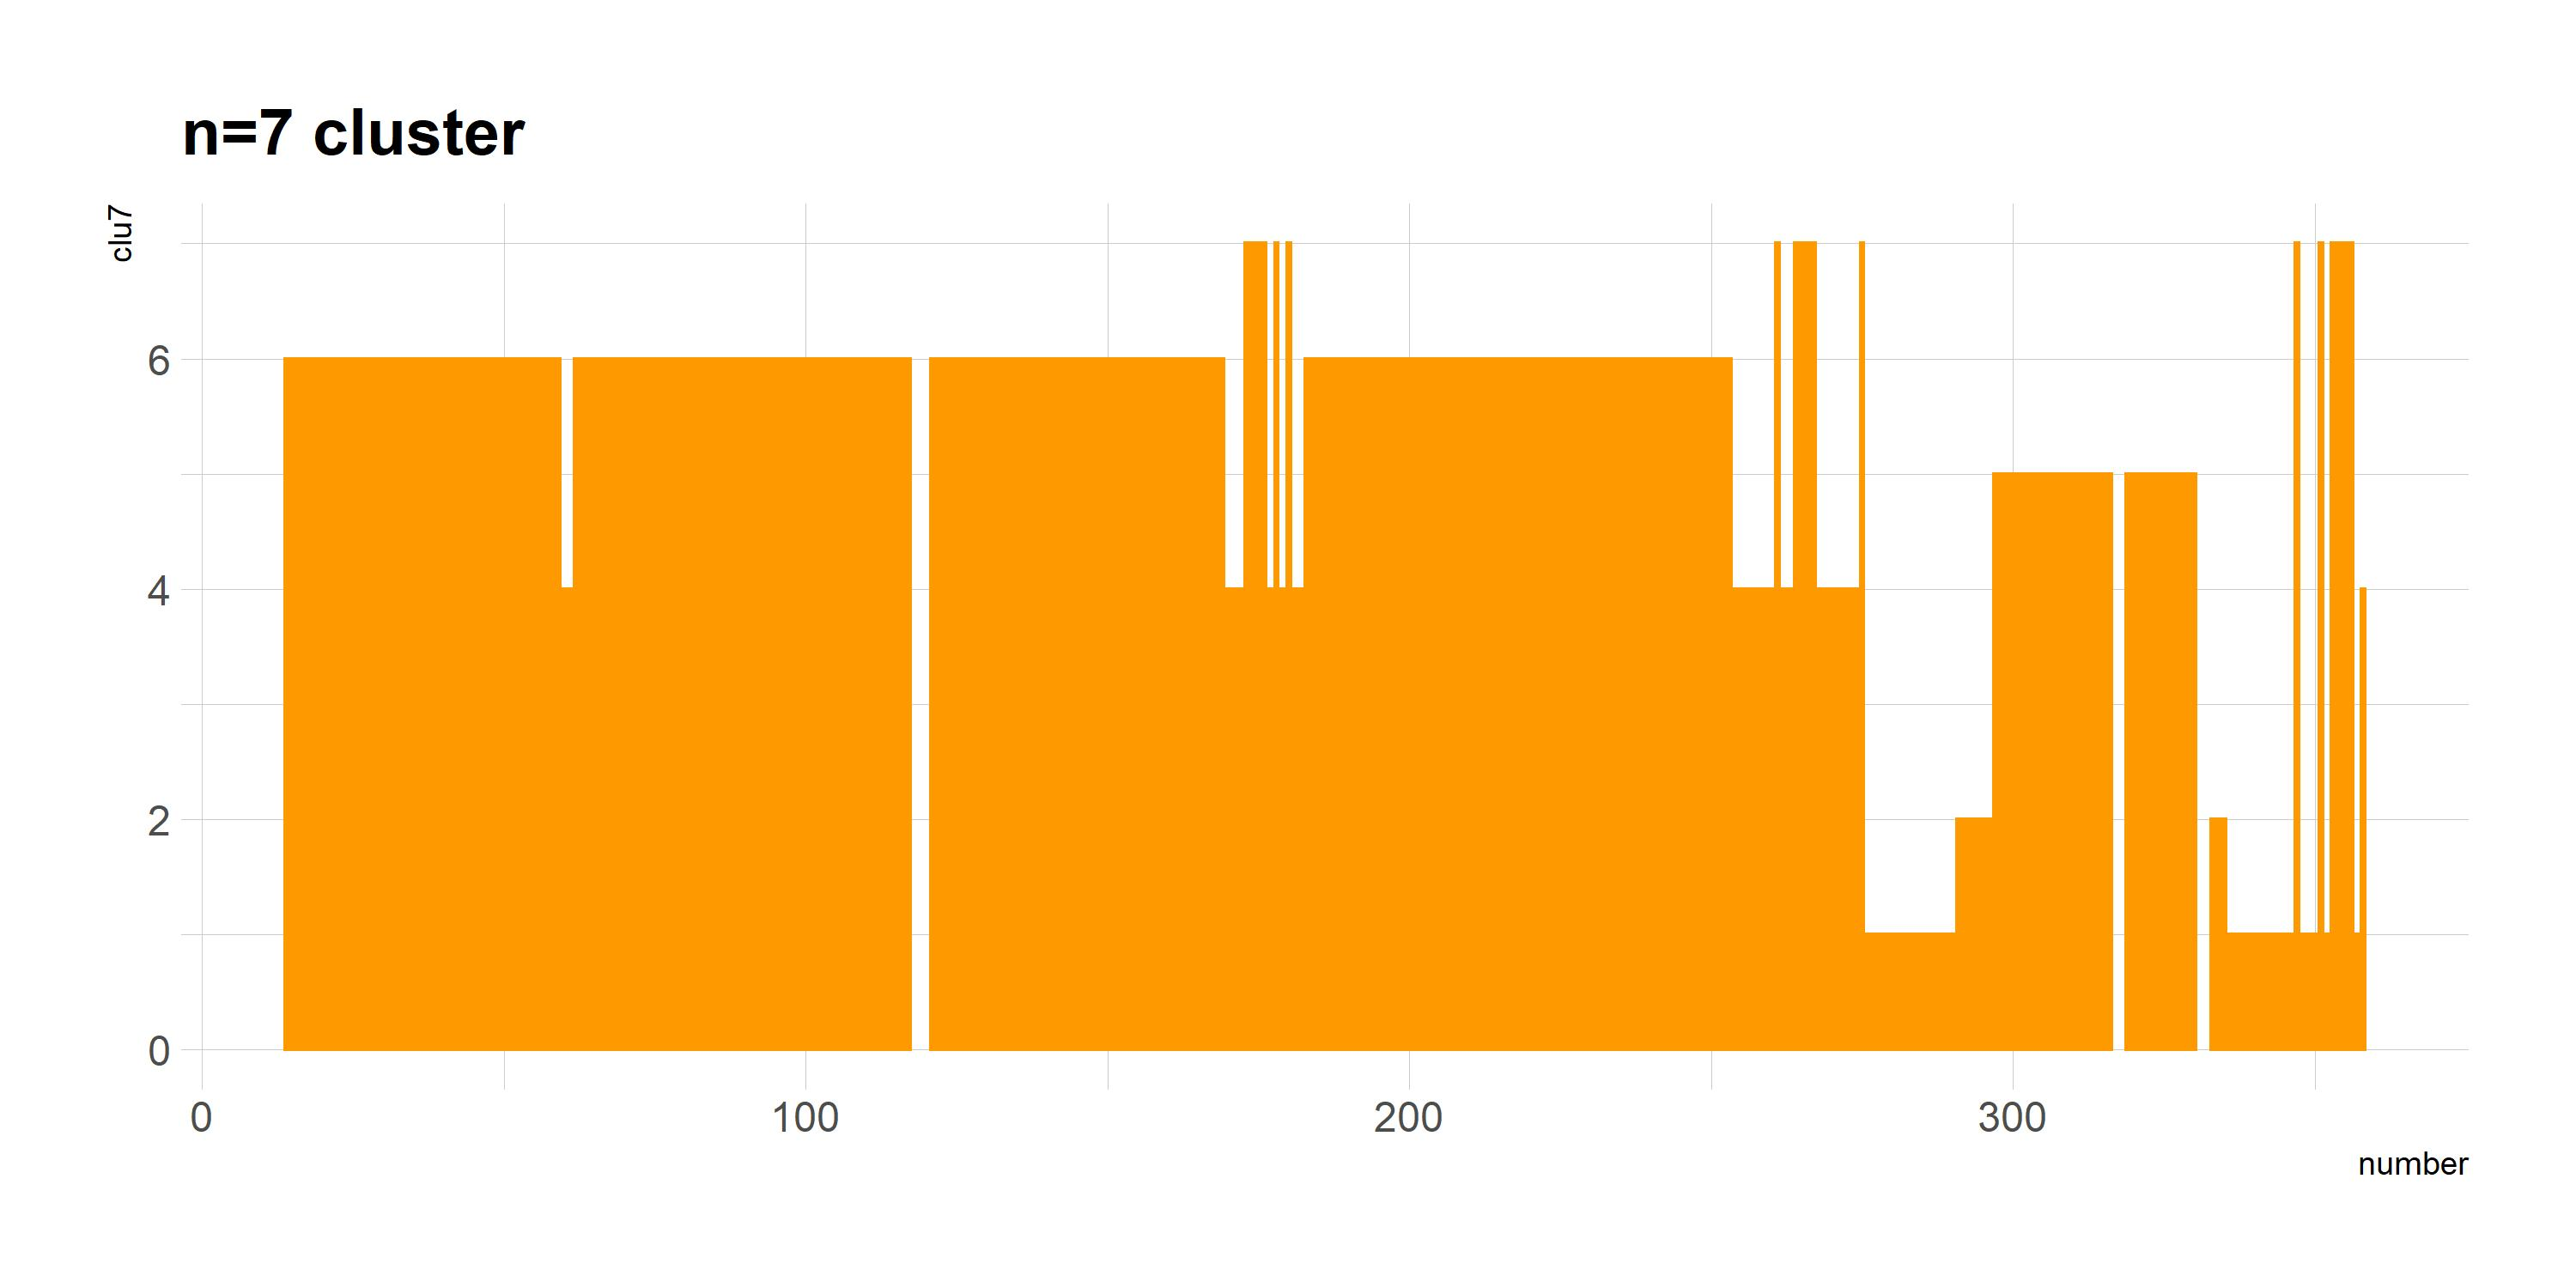
\includegraphics[width=6cm]{Figure/n7.jpg}
}
\quad
\subfigure[Performance of section line in cluster n=7(Shanghai) ]{
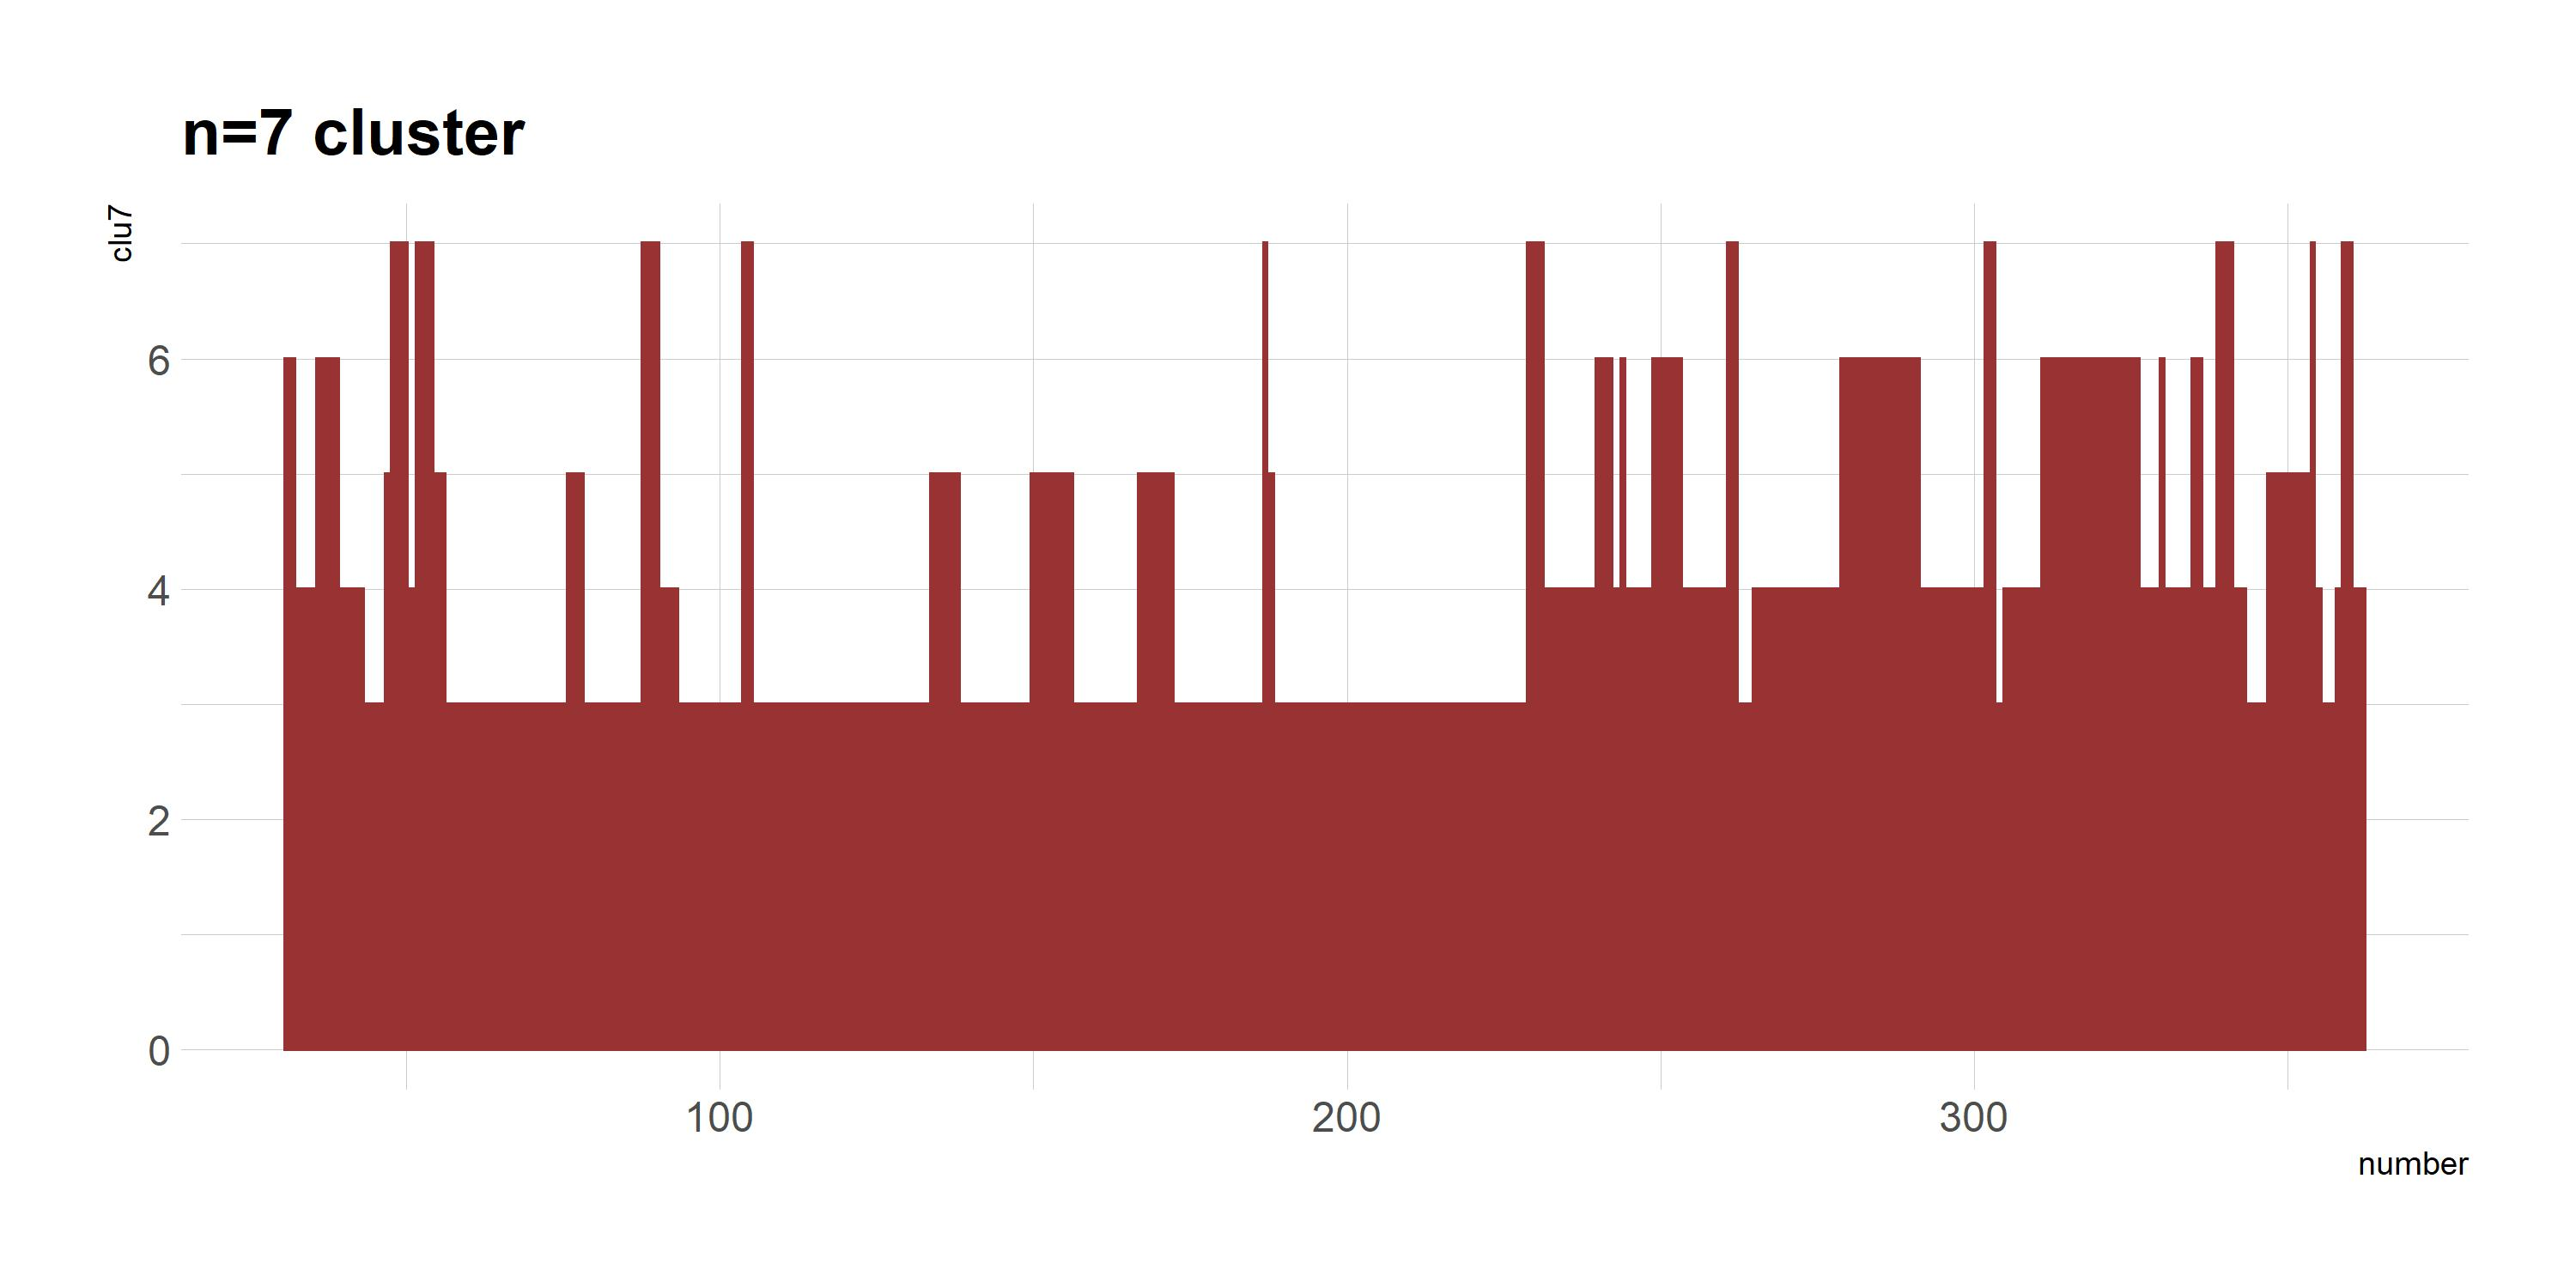
\includegraphics[width=6cm]{Figure/n7_sh.jpg}
}
\caption{The fluctuation of NT(Green) and DF(Red) values with section lines moving from south to north when n=7}
\label{section}
\end{figure}
%%%%%%%%%%%%%%%%%%%%%%%%%%%%%%%%%%%%

\subsubsection{Evaluation of socio-economic and environmental system}
As shown in Table \ref{description}, in order to evaluate the socio-economic and environmental system, 6 indicators from 2 systems were selected to assess the urban development and environmental outcomes.
%%%%%%%%%%%%%%%%%%%%%%%%%%%%%%%%%%%%%%%%%%%%%%%%%%%%%%%
\begin{table}[H]
\caption{The description of indicators in area evaluation}
\label{description}
\centering
\begin{tabular}{>{\hspace{0pt}}m{0.148\linewidth}>{\hspace{0pt}}m{0.6\linewidth}>{\centering\arraybackslash\hspace{0pt}}m{0.165\linewidth}} 
\hline
\multicolumn{1}{>{\centering\hspace{0pt}}m{0.148\linewidth}}{\textbf{Indcator}} & \multicolumn{1}{>{\centering\hspace{0pt}}m{0.6\linewidth}}{\textbf{Description}} & \textbf{Unit}  \\ 
\hline
\textbf{AL}                                                                     & Total area of construction land                                                    & \%             \\
\textbf{CL}                                                                     & Compactness of construction land                                                   & \%             \\
\textbf{NT}                                                                     & Nighttime data                                                                     &                \\
\textbf{NDVI}                                                                   & Normalized Difference Vegetation Index                                             &                \\
\textbf{NPP}                                                                    & Net Primary Production                                                             & $gc/(m^{2}*a)$      \\
\textbf{PM2.5}                                                                  & Air pollutants                                                                     & $\mu g/m^{3}$          \\
\hline
\end{tabular}
\end{table}
%%%%%%%%%%%%%%%%%%%%%%%%%%%%%%%%%%%%%%%%%%%%%%%%%%%%%%%
\subsubsubsection{Socio-economic system}
In order to evaluate the urban development of each case study city 3 dimensions of socio-economic indicators should be used to assess from the point of land development intensity. 
The first dimension is AL, which would refer to the total area of construction land in the grid of $300m \times 300m$ in this study. It could also be expressed as the area proportion of construction land in the assessing unit.\\
\begin{equation}
AL=\frac{A}{T}
\end{equation}
Where A is the total area of construction land; T is the assessing area.\\

The second dimension would be CL, which may refer to the compactness of construction land. According to research, it could define as the ratio of the area to the perimeter \parencite{peng_integrating_2020}. The calculation of CL would be chosen because of its high applicability and simple calculation process.\\
\begin{equation}
CL=\frac{A}{C}
\end{equation}
Where C is the length of individual construction land in the assessing unit.\\

The third dimension would be Nighttime light data. Since socio-economic activity could be positively correlated with the nighttime light data, NT could be also used to evaluate the socio-economic system. Compared with other indicators, since there has been a huge distance between the maximum value of NT and the medium value of NT, the study would take logarithms of the lighting data($NT_{log}$) as the assessment indicator.\\

What‘s more, with the resolution of $300m \times 300m$ in NT, in order to calculate the CL and AL value, the study would statistics in $300m \times 300m$ to ensure the standard of socio-economic data.\\

\subsubsubsection{Environmental system}
When it comes to the topic of climate change and air quality, 3 dimensions of indicators should be used to represent environmental outcomes.\\

The first dimension is NDVI, which can be referred to biodiversity from ecosystem service. The second dimension is NPP, with carbon fixation perspective. The last dimension is PM2.5, which have a different aspect of air pollution.\\

\subsubsubsection{Normalization of evaluation value}
In order to compare the socio-economic system and the environmental system from a comprehensive perspective, the indicators of each system would be integrated by means of normalization. The integration method would be shown as below:\\

\begin{equation}
IN_{i j norm}= \begin{cases}\frac{IN_{i j}}{\max IN_{i j}} & IN_{i j} \text { shows the larger the better } \\ \frac{\min IN_{i j}}{IN_{i j}} & IN_{i j} \text { shows the smaller the better } \\ \frac{\min \left(IN_{i j}, IN_{j}^{0}\right)}{\max \left(IN_{i j}, IN_{j}^{0}\right)} & \mathrm{IN}_{j}^{0} \text { is the ideal value with respect to } IN\end{cases}\\
\end{equation}
\begin{equation}
S_{i}=\frac{1}{n} \sum_{j=1}^{n} IN_{i j norm}
\end{equation}
Where $IN_{i j}$ is the value of each indicator, $S_{i}$ is the value of the normalization index.\\

When exploring each indicator, it was found that all the data except PM2.5 showed the larger the better trend. On the contrary, indicator PM2.5 showed the trend of the smaller the better. When using the formula to integrate each indicator, the study would generate socio-economic index and environmental index ranging from 0 to 1\\
 

\newpage
\section{Result}

\subsection{Spatial distribution of urban fringe area}
\subsubsection{Guangzhou}
The results from Figure \ref{fringe}a show that the spatial distribution of urban area in Guangzhou was mostly located in the central area, accounting for 20.43\% of the total research area. While in the northern and southern part of the area, there was only a small amount of urban area. The suburban area accounted for 58.73\% of the total area and was mostly located in the northern part of the area. The land use type of suburban was mostly woodland. Besides, the urban fringe area was mostly developed around the socio-economic center in the central part of the city, accounting for 20.84\% of the total area. Compared with other areas, urban fringe area could also be found in the border area of the city. This was mainly because the influence of the neighboring cities. Frequent business exchanges and road facilities in this area have changed the character of the area, Besides, this may also be due to the urban sprawl and urbanization of the neighboring cities, which affects the regional changes of the study area.\\

The land use type of the area was mostly woodland in the northern part of the area. Most of the urban area was developed around woodland. The urban area in the region was very fragmented and the connectivity of the area would be low. By comparing the urban area in the urban center, it can be seen that as the northern area becomes more distant from the urban center, the agglomeration and the area of the urban area would become smaller at a very fast rate. This was also because there were a huge number of ecological reserves in the northern area, which would be far away from the central area. The development of urban area would inevitably have serious impacts on the ecosystem service function of the ecological area. In the meanwhile, the land use type of suburban area would be farmland and woodland in the northern part and acting as the dominant area. With reservoirs in this kind of area, suburban area in the northern part provides the necessary support for water conservation and soil conservation of the urban ecosystem. Besides, in terms of spatial connection, the suburban area in the northern part surrounds a small amount of urban area. In this case, the development of urban development in the northern part would be relatively slow.\\

The urban area in the south of the city was even less than the northern area. What is worth mentioning is that since the southern area was connected to the South China Sea and part of the river passes through it, as the center of the development, the urban area of the region made a great development depended on the river. The urban fringe area was also denser in the southern part of the city than in other areas. The land use type in the southern area was farmland, and as a water-dependent development area there was also potential for commercial development as an urban focus.\\

As the center of socio-economic area, the central area was the most concentrated area in the urban area. Since the central area was crossed by rivers, it would maintain a good living environment and also sustain the economic development of the city. It could be seen that there are many urban fringe areas around the rivers in the central area, which could further prove that the development of this type of cities was driven by water resources.\\

%%%%%%%%%%%%%%%%%%%%%%%%%%%%%%%%%%%%
\begin{figure}[H]
\centering
\subfigure[Guangzhou]{
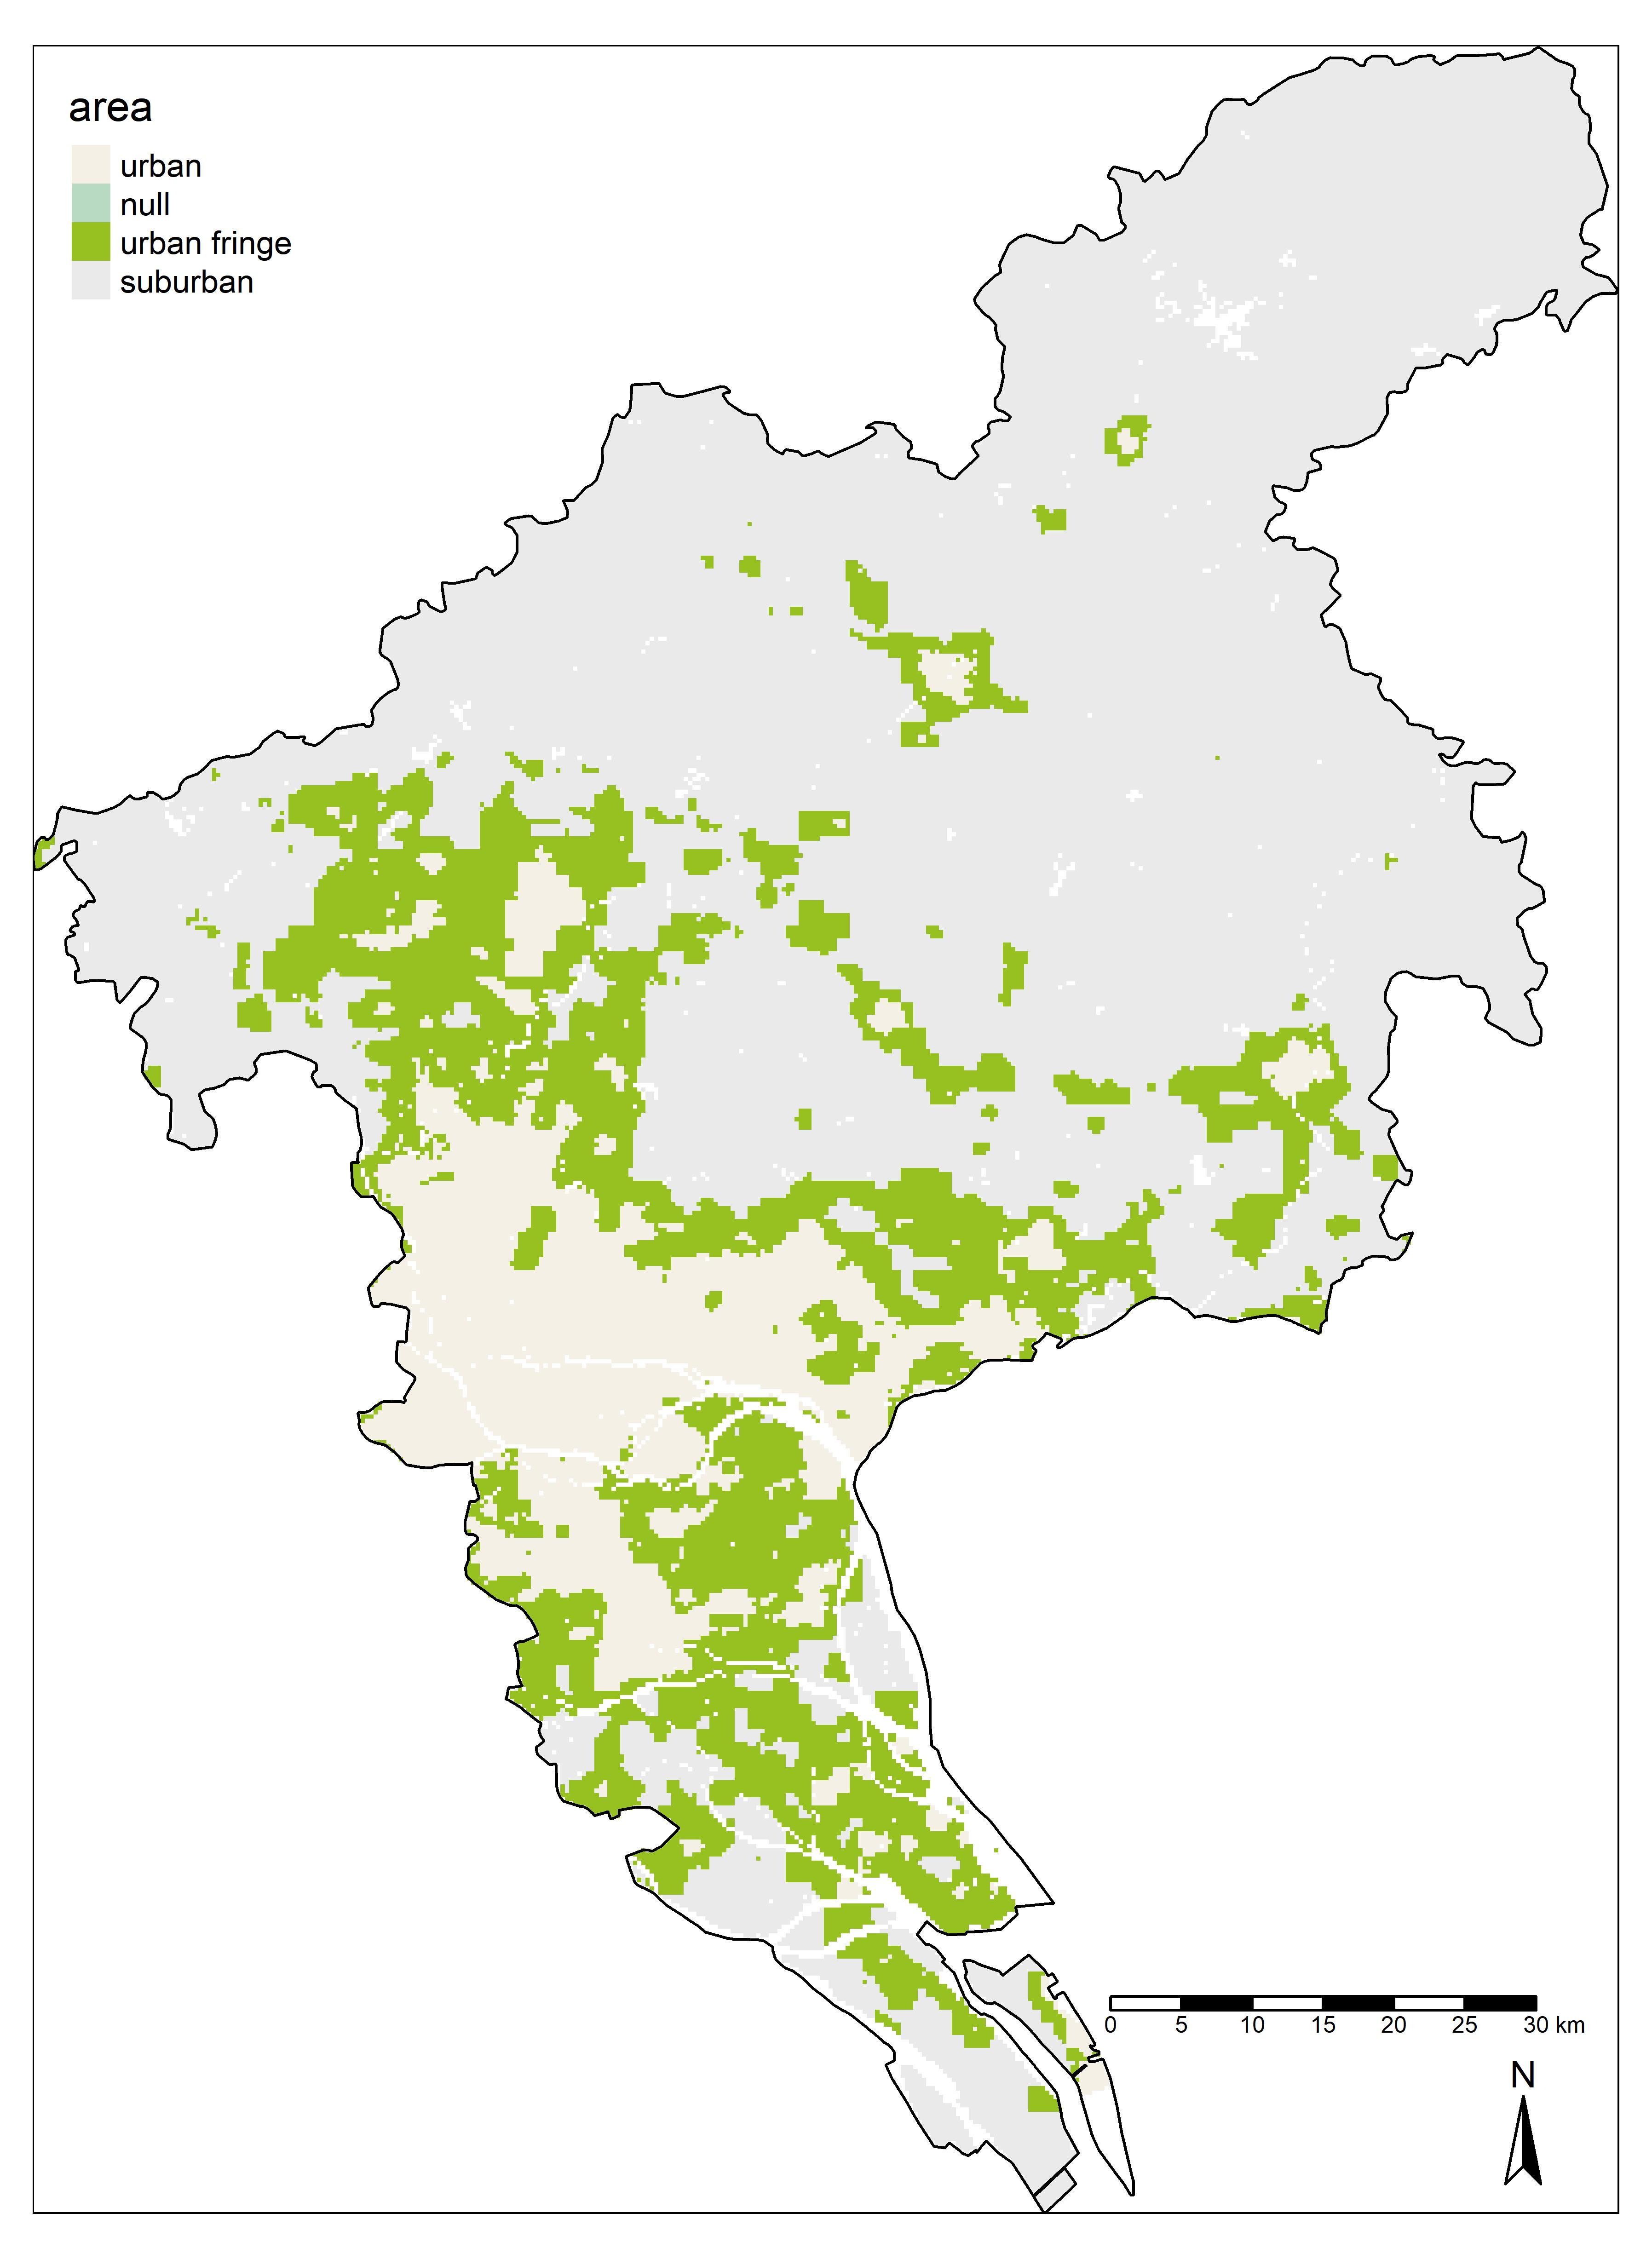
\includegraphics[width=6cm]{Figure/urbanfringegz_0821.jpg}
}
\quad
\subfigure[Shanghai]{
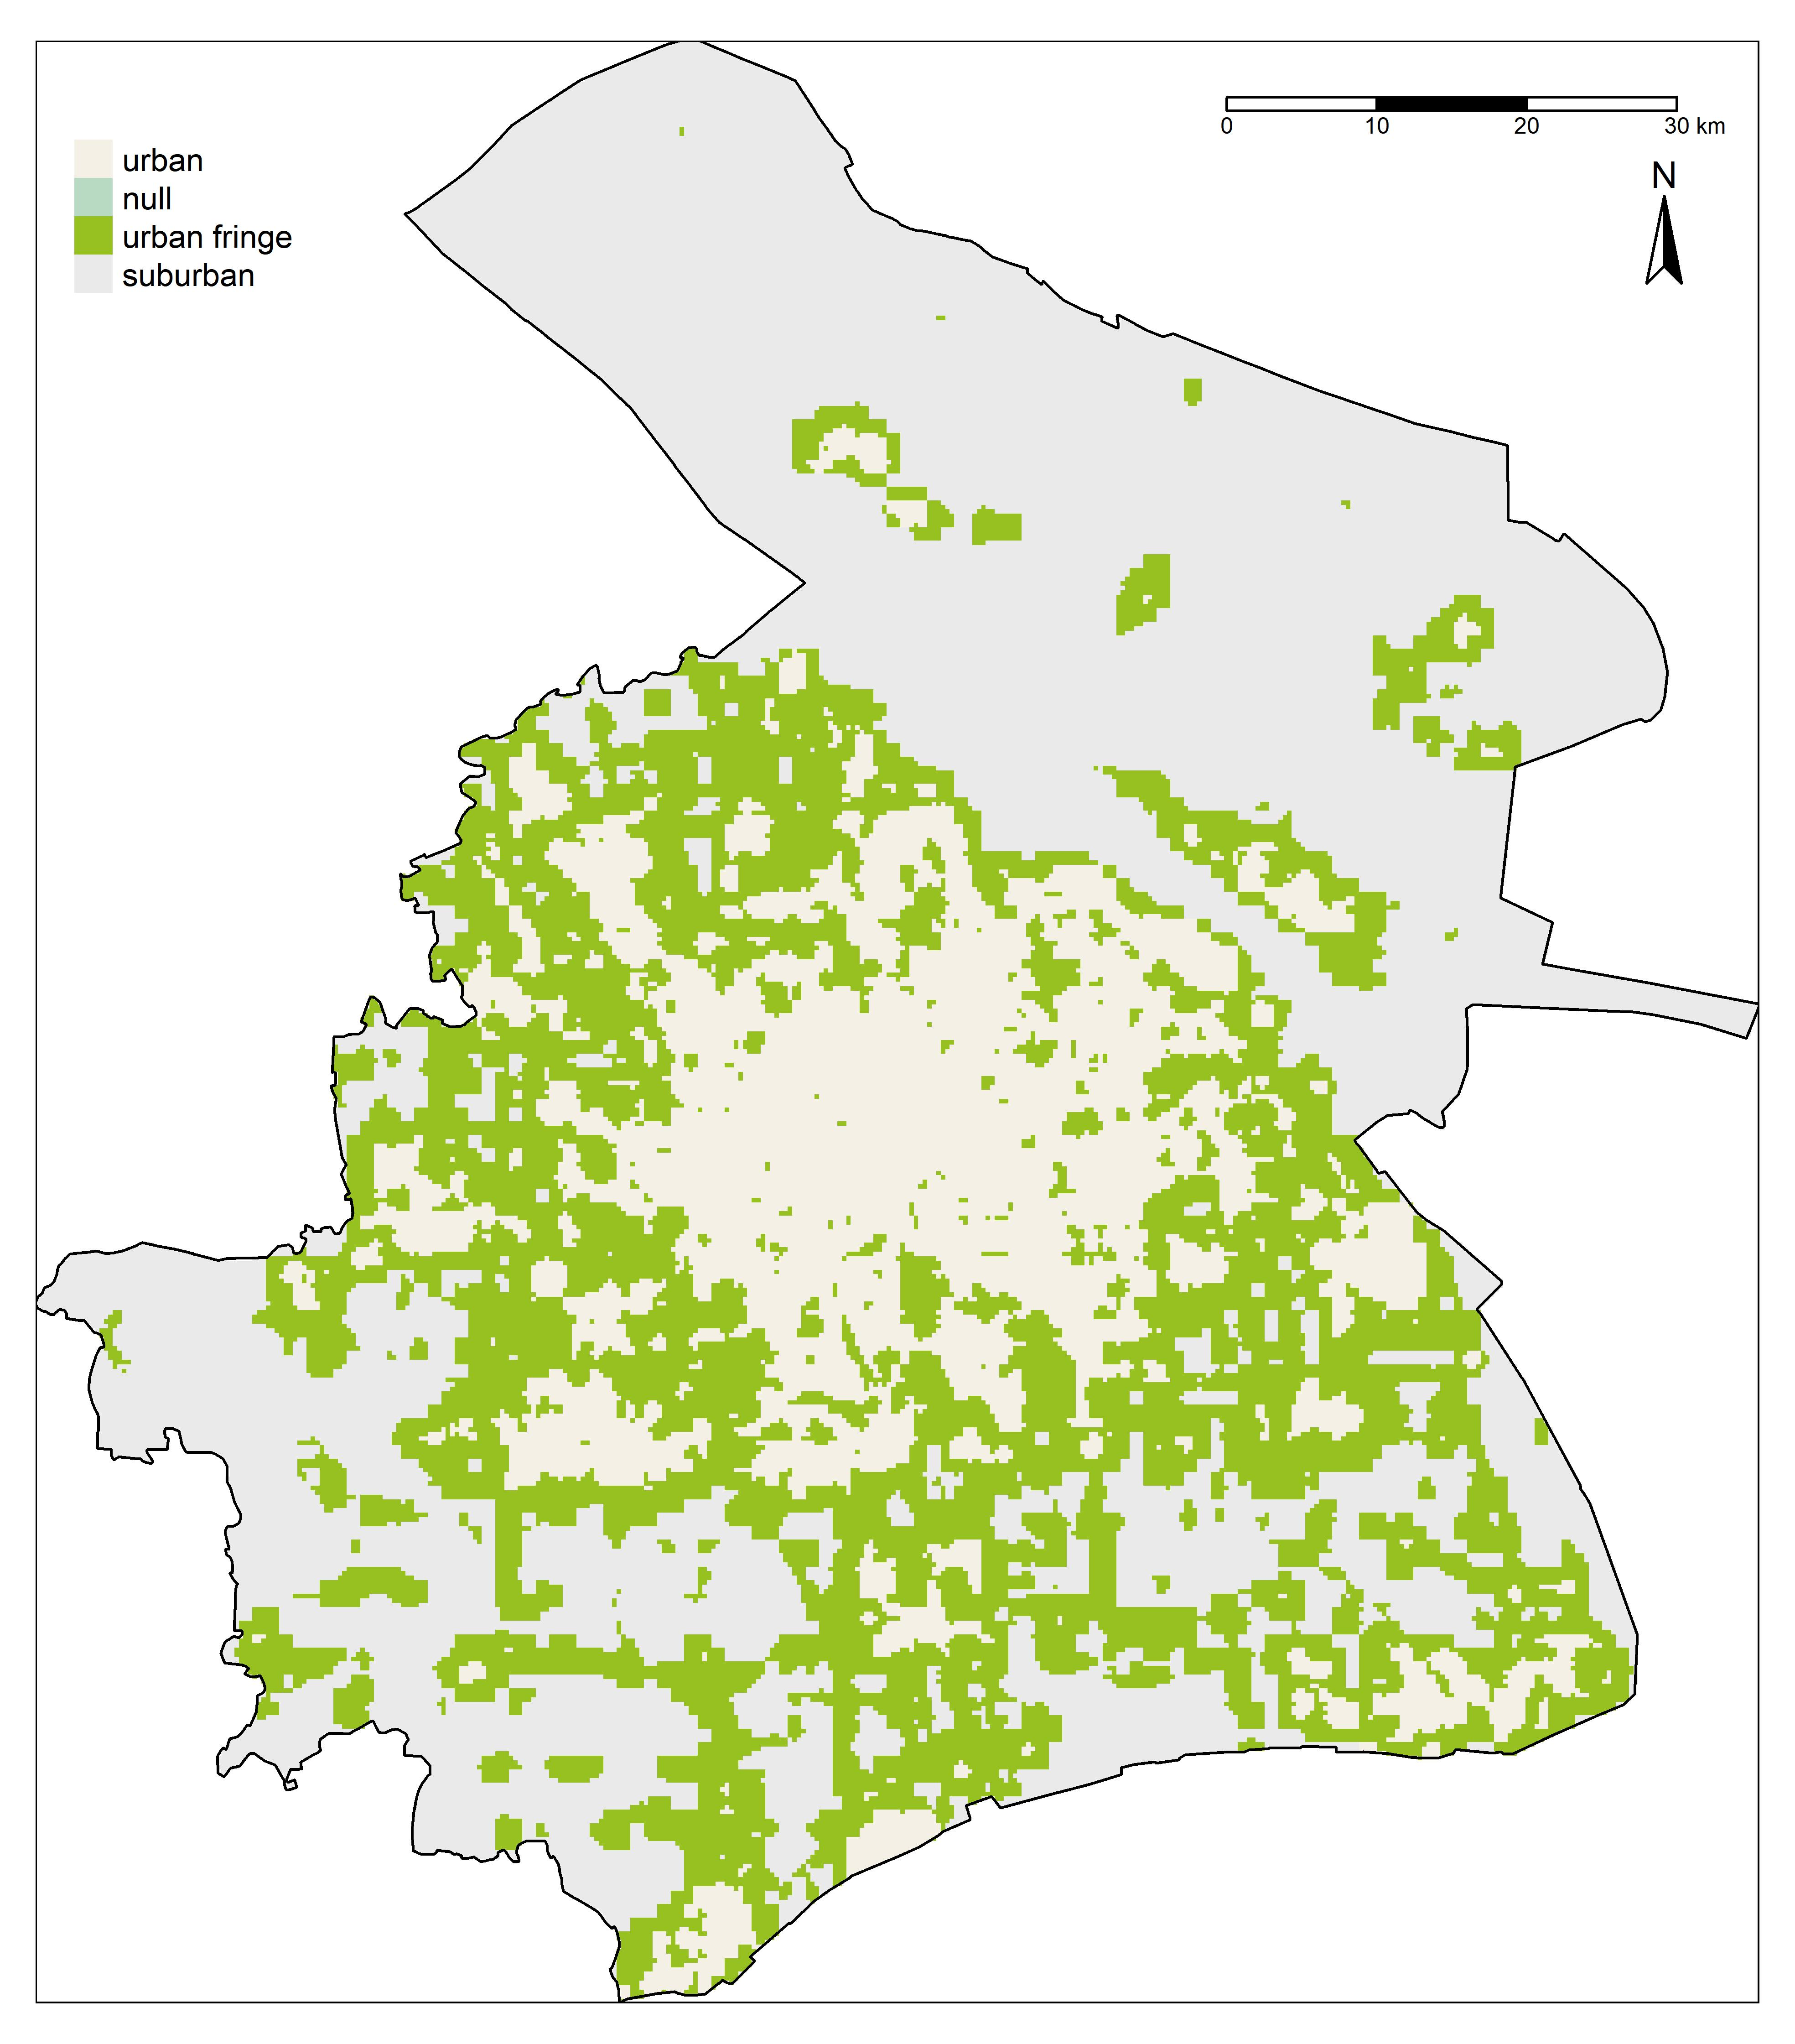
\includegraphics[width=7cm]{Figure/urbanfringe_sh0821.jpg}
}

\caption{The distribution of urban area, urban fringe area and suburban area}
\label{fringe}
\end{figure}
%%%%%%%%%%%%%%%%%%%%%%%%%%%%%%%%%%%%

\subsubsection{Shanghai}
The spatial layout of Shanghai's urban area (Figure \ref{fringe}b) was similar to that of Guangzhou, which was mainly concentrated in the central area of the city, accounting for 19.80\% of the total area. The urban fringe area, due to its distance from the urban area, was concentrated in the central and southern part of the city, accounting for 31.68\% of the total area. Suburban area was the largest area in the city and it was mainly located in the northern islands of the city. Suburban area accounted for 48.52\% of the total area.\\

When it comes to the north of the city, the two islands in the north were separated from the central area by a river because of their geographical location. Therefore, the area was not closely connected in terms of transportation and it has not been developed much in urban construction process in these years. It is clear that the urban fringe area in the northern area was the smallest part of the city and most of the land was woodland, which would be a difficult area to develop.\\

As the central area of the city, the central part of Shanghai plays an important role as the economic center, so the level of urban construction has been generally high. Most of the land types in this area were construction land. Consequently, there have been relatively more urban fringe areas.\\

As the key area for economic development in Shanghai, the southern part of the city, has identified a large number of urban fringe areas, which were distributed in a strip-like pattern in the spatial layout. This type of area would be spatially distributed in the form of strips, which could be interspersed with urban area and suburban to form a network spatial shape.\\


\subsection{Descriptive statistics}

%%%%%%%%%%%%%%%%%%%%%%%%%%%%%%%%%%%%%%%%%%%%%%%%%%%%%%%

\begin{table}[H]
\caption{The general statistics of indicators from 2 systems in Guangzhou and Shanghai}
\label{statistics}
\centering
\begin{tabular}{>{\hspace{0pt}}m{0.25\linewidth}>{\hspace{0pt}}m{0.107\linewidth}>{\hspace{0pt}}m{0.073\linewidth}>{\hspace{0pt}}m{0.109\linewidth}>{\hspace{0pt}}m{0.09\linewidth}>{\hspace{0pt}}m{0.073\linewidth}>{\hspace{0pt}}m{0.127\linewidth}} 
\hline
\multicolumn{1}{>{\hspace{0pt}}m{0.25\linewidth}|}{}                  & \multicolumn{3}{>{\centering\hspace{0pt}}m{0.289\linewidth}|}{\textbf{Guangzhou}}                & \multicolumn{3}{>{\centering\arraybackslash\hspace{0pt}}m{0.29\linewidth}}{\textbf{Shanghai}}  \\ 
\cline{2-7}
\multicolumn{1}{>{\hspace{0pt}}m{0.25\linewidth}|}{\textbf{Indcator}} & \textbf{Max} & \textbf{Min} & \multicolumn{1}{>{\hspace{0pt}}m{0.109\linewidth}|}{\textbf{Mean}} & \textbf{Max} & \textbf{Min} & \textbf{Mean}                                                    \\ 
\hline
\textbf{Socio-economic index}                                          & 0.97         & 0            & 0.21                                                               & 0.92         & 0            & 0.3                                                              \\
\textbf{AL}                                                            & 1            & 0            & 0.18                                                               & 1            & 0            & 0.30~                                                            \\
\textbf{CL}                                                            & 75.87        & 0            & 21.78                                                              & 76.23        & 0            & 13.82                                                            \\
\textbf{NT}                                                            & 331.15       & 0            & 8.19                                                               & 371.3        & 0            & 14.09                                                            \\
\textbf{Environmental index}                                           & 0.97         & 0.24         & 0.64                                                               & 0.92         & 0.12         & 0.58                                                             \\
\textbf{NDVI}                                                          & 0.85         & 0            & 0.55                                                               & 0.85         & 0            & 0.43                                                             \\
\textbf{NPP}                                                           & 14141        & 0            & 6484.2                                                             & 9862         & 0            & 3343.16                                                          \\
\textbf{PM2.5}                                                         & 34.6         & 23.5         & 28.22                                                              & 45.9         & 26.4         & 32.99                                                            \\
\hline
\end{tabular}
\end{table}

%%%%%%%%%%%%%%%%%%%%%%%%%%%%%%%%%%%%%%%%%%%%%%%%%%%%%%%

\subsubsection{Socio-economic index}
Figure \ref{ugz} and \ref{ush} showed the performance of each indicator from urban development system in 2019 from Guangzhou and Shanghai. Table \ref{statistics} showed the general statistics of each indicator including average value in these two cities. Socio-economic index in the large area of high-values from Guangzhou was concentrated in the central part of the city. It was worth noting that the continuous and high-value areas were mostly located on both sides of the rivers in the central part. Compared to this, the southern areas were fragmented but the high-value areas were still evenly distributed over the spatial area. As we could see within the northern area, there were certain variations, with only a few high-value spaces in the northeast part due to the influence of woodland and other ecological green spaces. While in the northwest part of the area, there were fragmented but concentrated areas near the central river. Through the analysis of the socio-economic index, we could further consider a method to connect this area through land consolidation and other measures, so that the urban space could be used more efficiently.\\

When it comes to Shanghai, the socio-economic index with a large range of high-value areas was concentrated in the central part of the city near the south of the river. The urban construction areas in the central area would show a concentrated and centralized pattern. Besides, the northern part of the city had almost no high-value areas due to the poor river connectivity with the central part of the city. What is worth mentioning is that the areas with high index were all close to the river and the southern part of the central part of the city.\\

When comparing the difference between Guangzhou and Shanghai, The highest values in Guangzhou are higher than those in Shanghai. Guangzhou had relatively few high-value areas In terms of spatial distribution, and they were also very concentrated in the central area. The high-value areas in Shanghai were distributed evenly in most of the city-wide areas. This also indicated that Guangzhou's development in some areas was relatively more prominent than in other areas, while SH showed more nodal and core development characteristics within the areas due to its uniform distribution. In addition, the average value of Shanghai socio-economic index was larger than that of Guangzhou, which means that the economic level of Shanghai was much higher than that of Guangzhou.\\

%%%%%%%%%%%%%%%%%%%%%%%%%%%%%%%%%%%%
\begin{figure}[H]
\centering
\subfigure[Socio-economic index]{
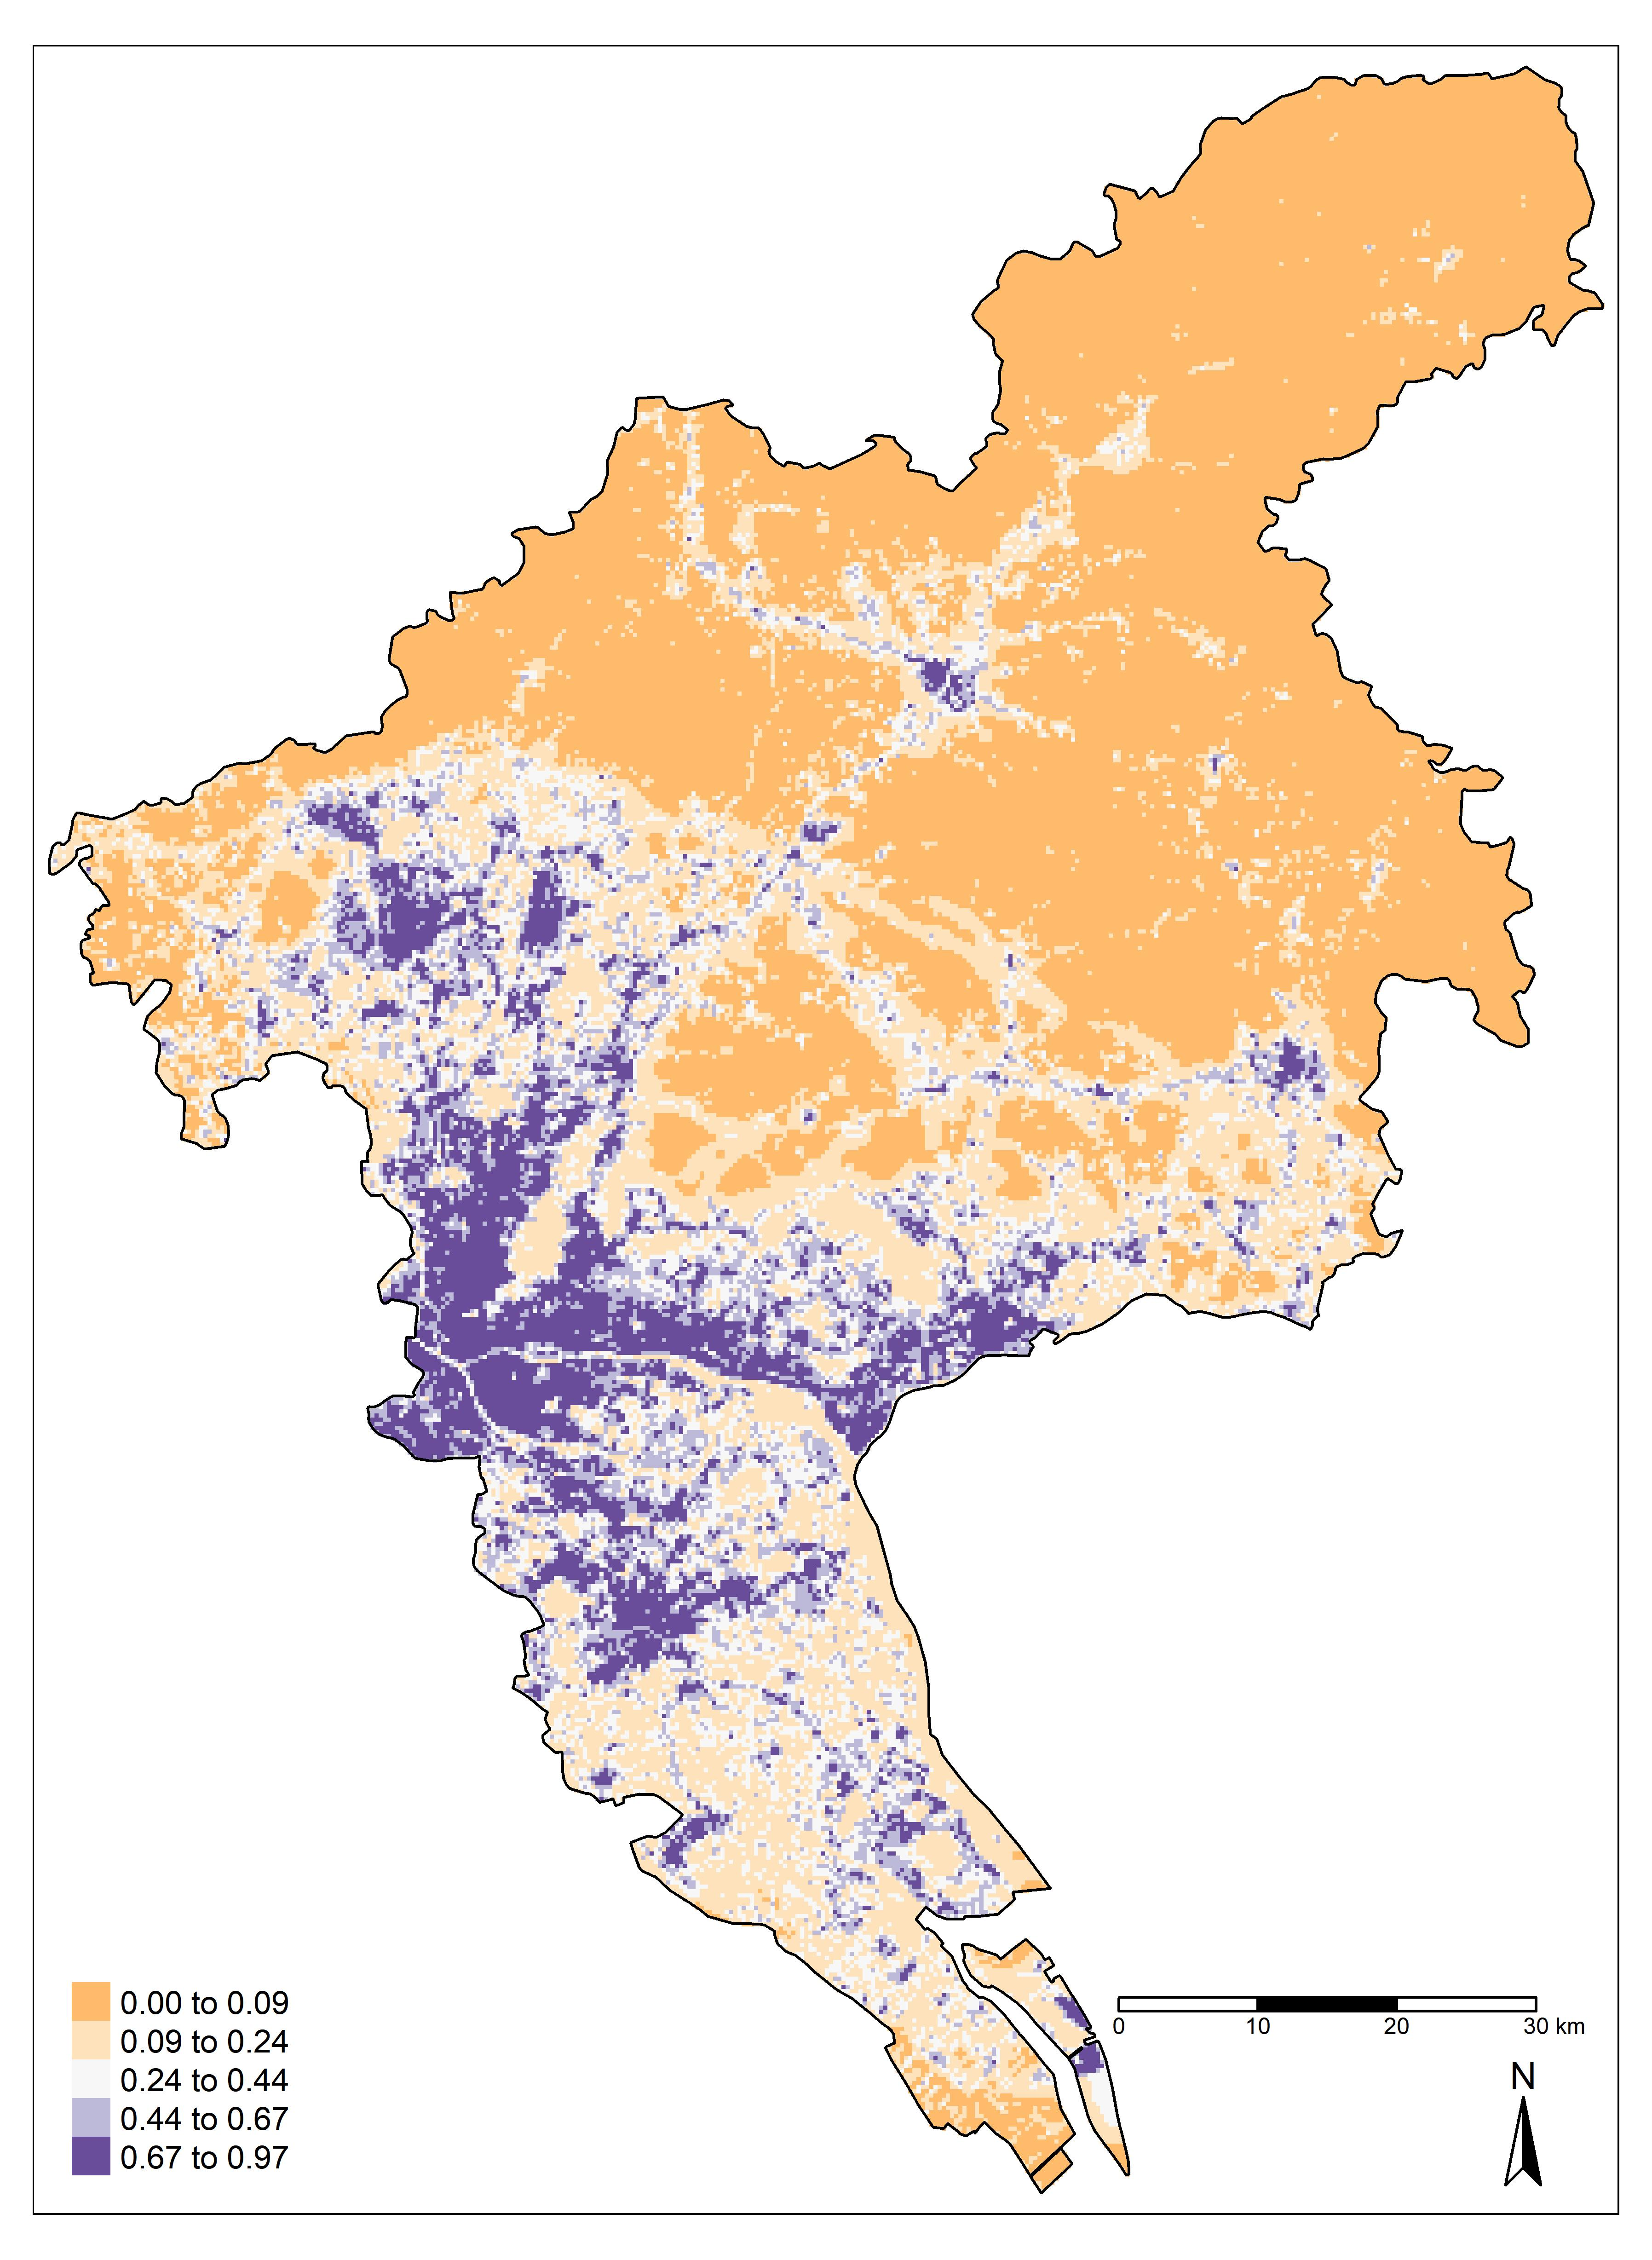
\includegraphics[width=6cm]{Figure/ugz.jpg}
}
\quad
\subfigure[AL]{
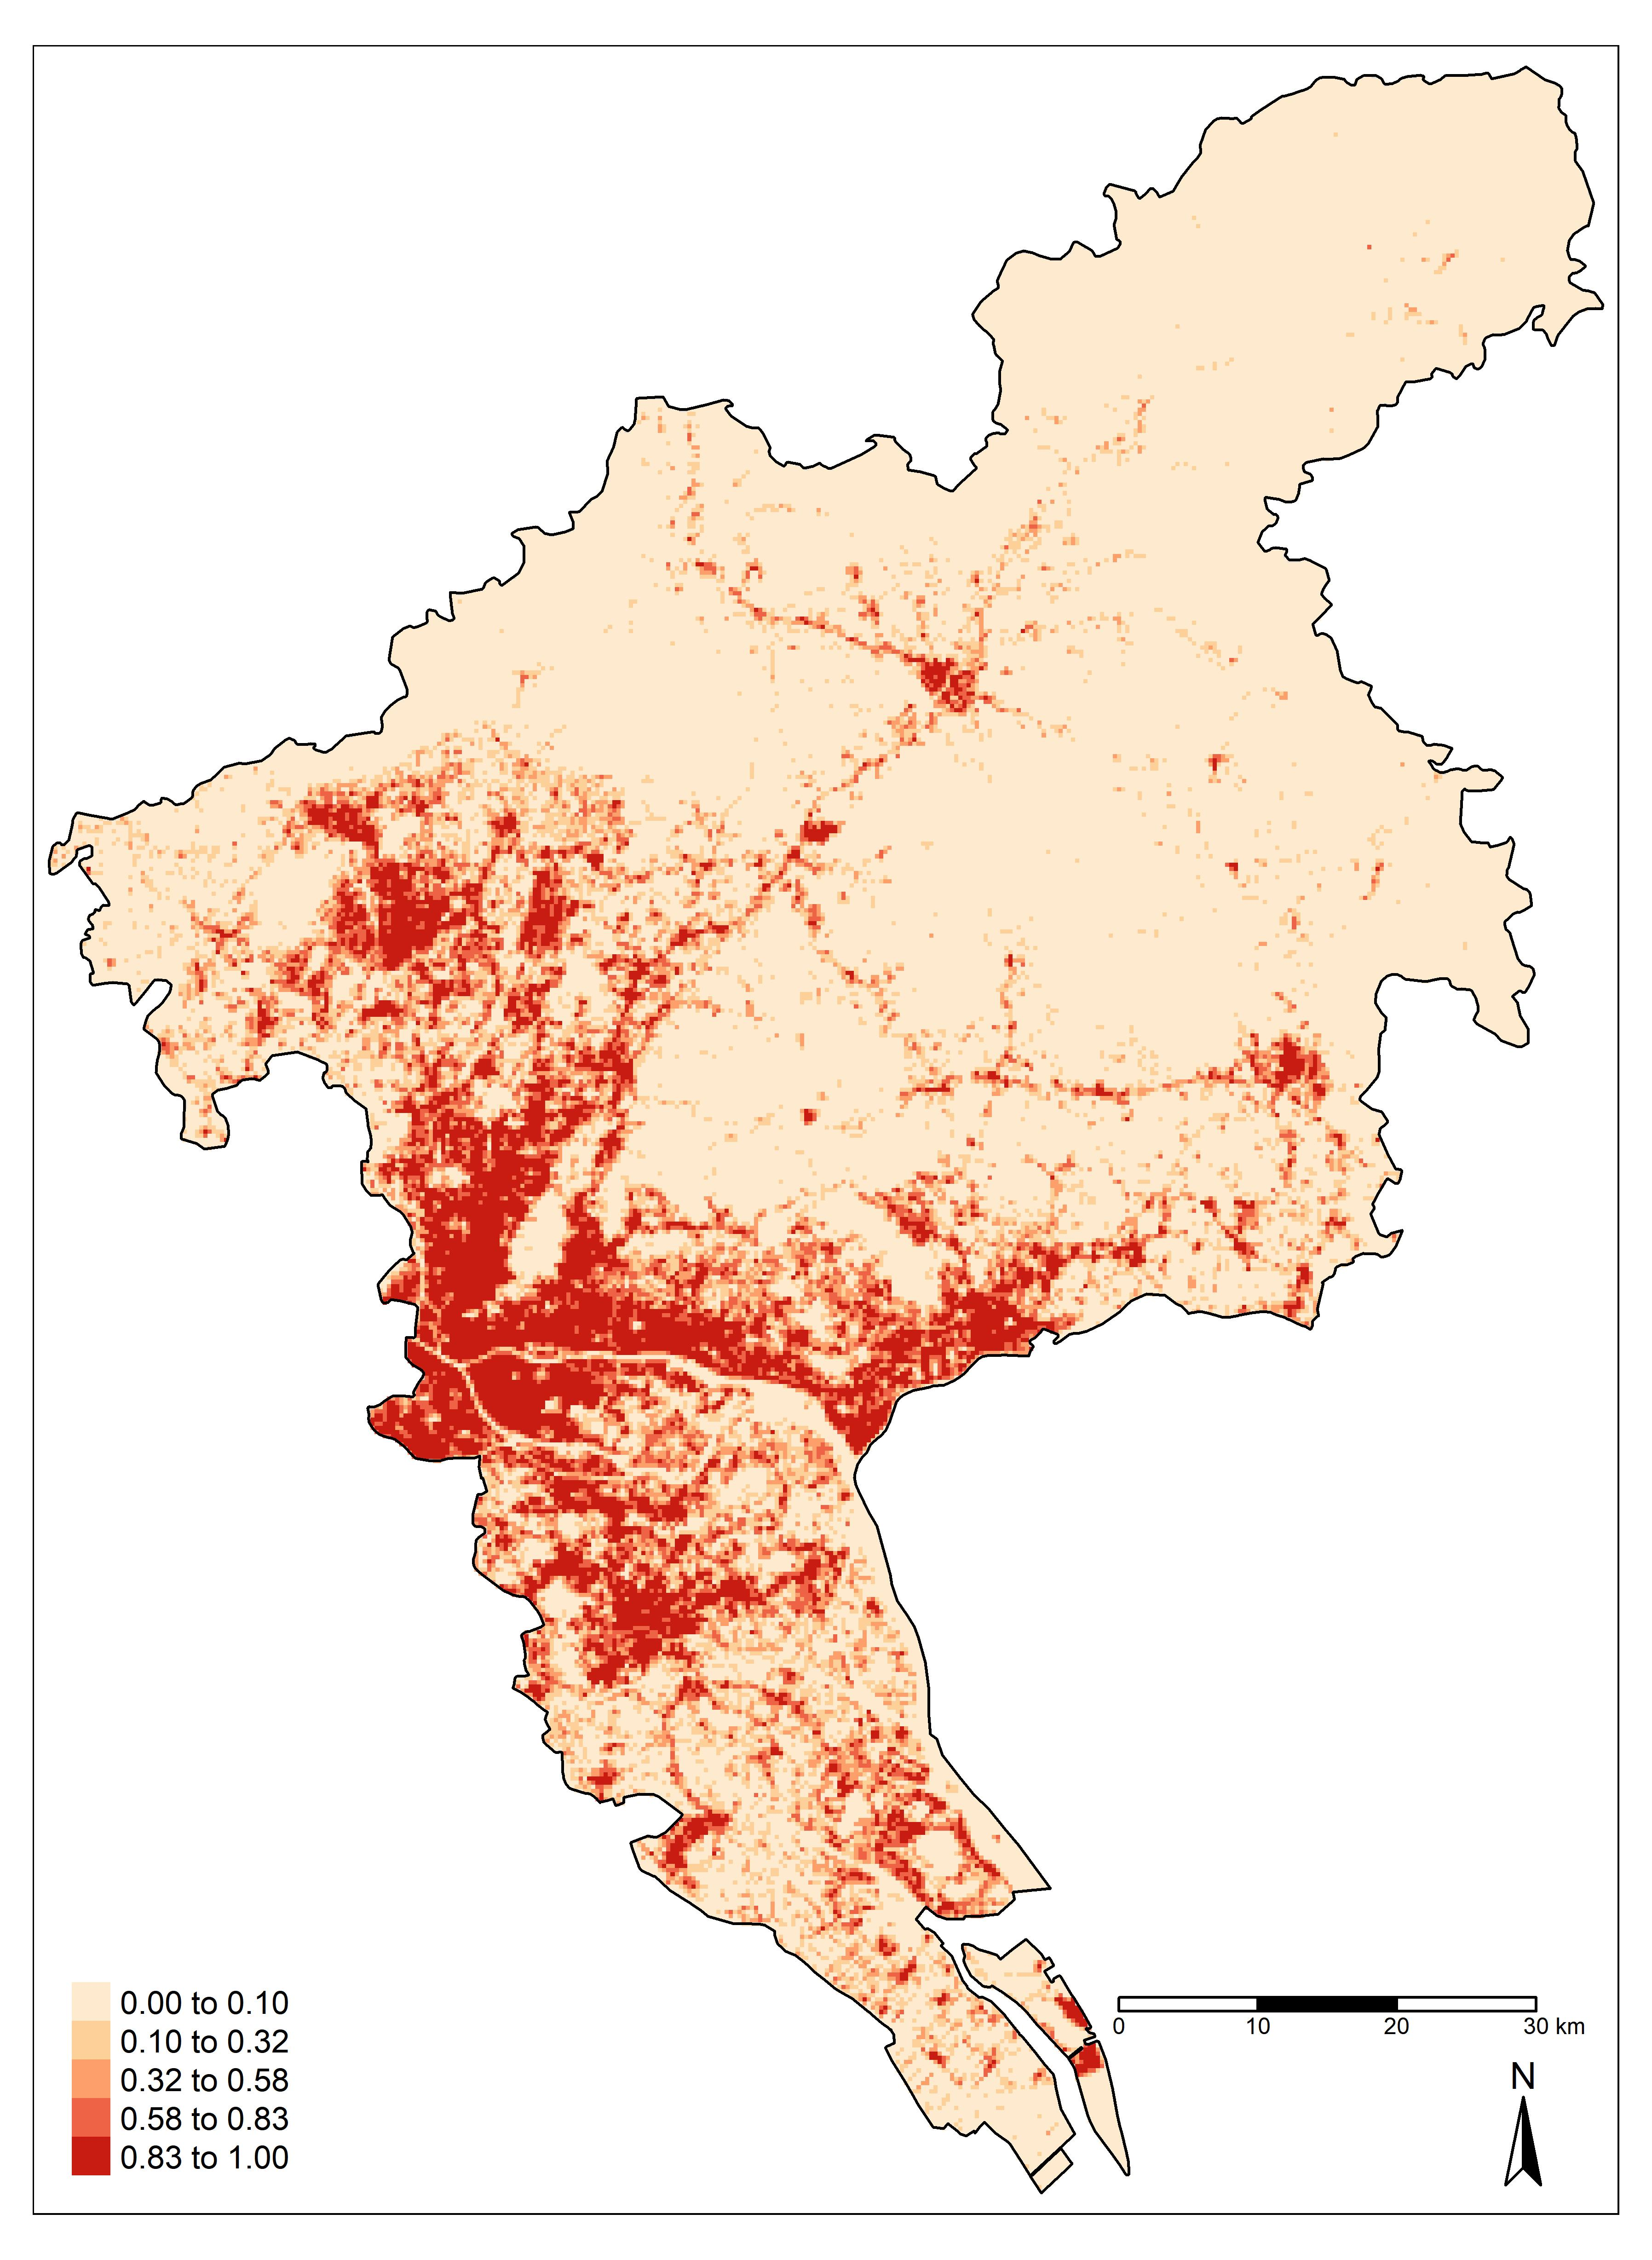
\includegraphics[width=6cm]{Figure/area_gz.jpg}
}
\quad
\subfigure[CL]{
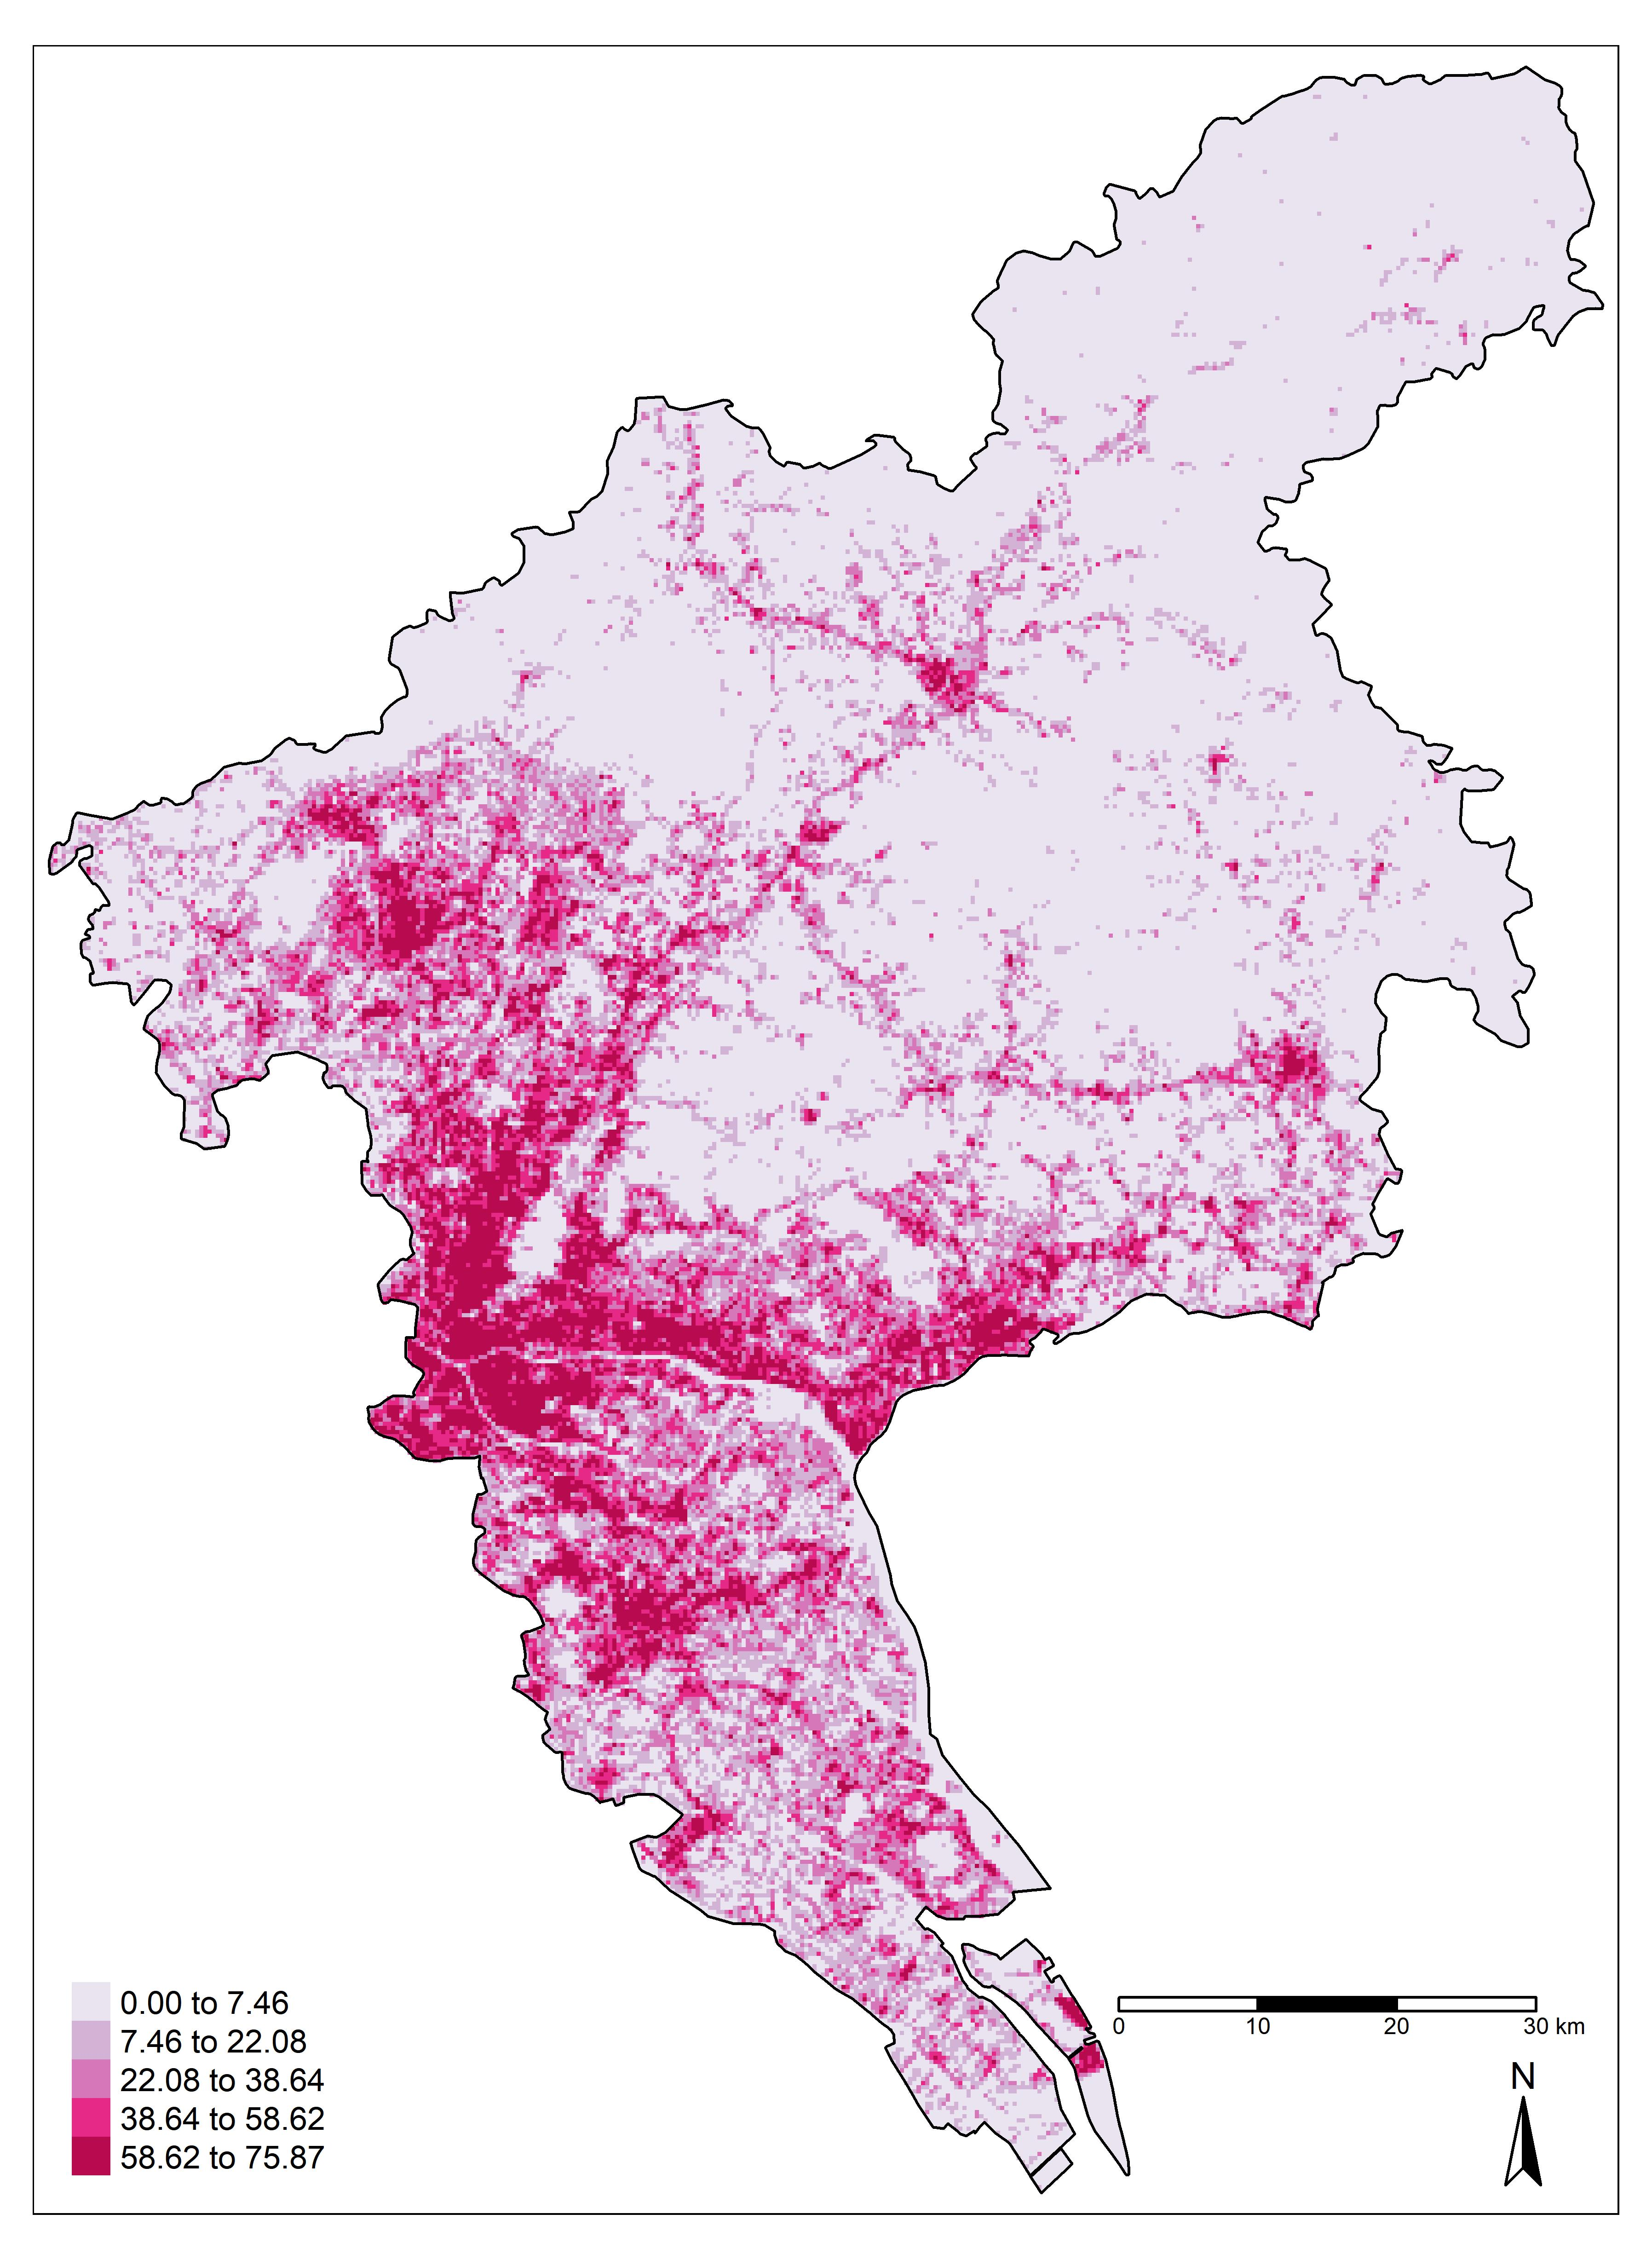
\includegraphics[width=6cm]{Figure/length_gz.jpg}
}
\quad
\subfigure[NT]{
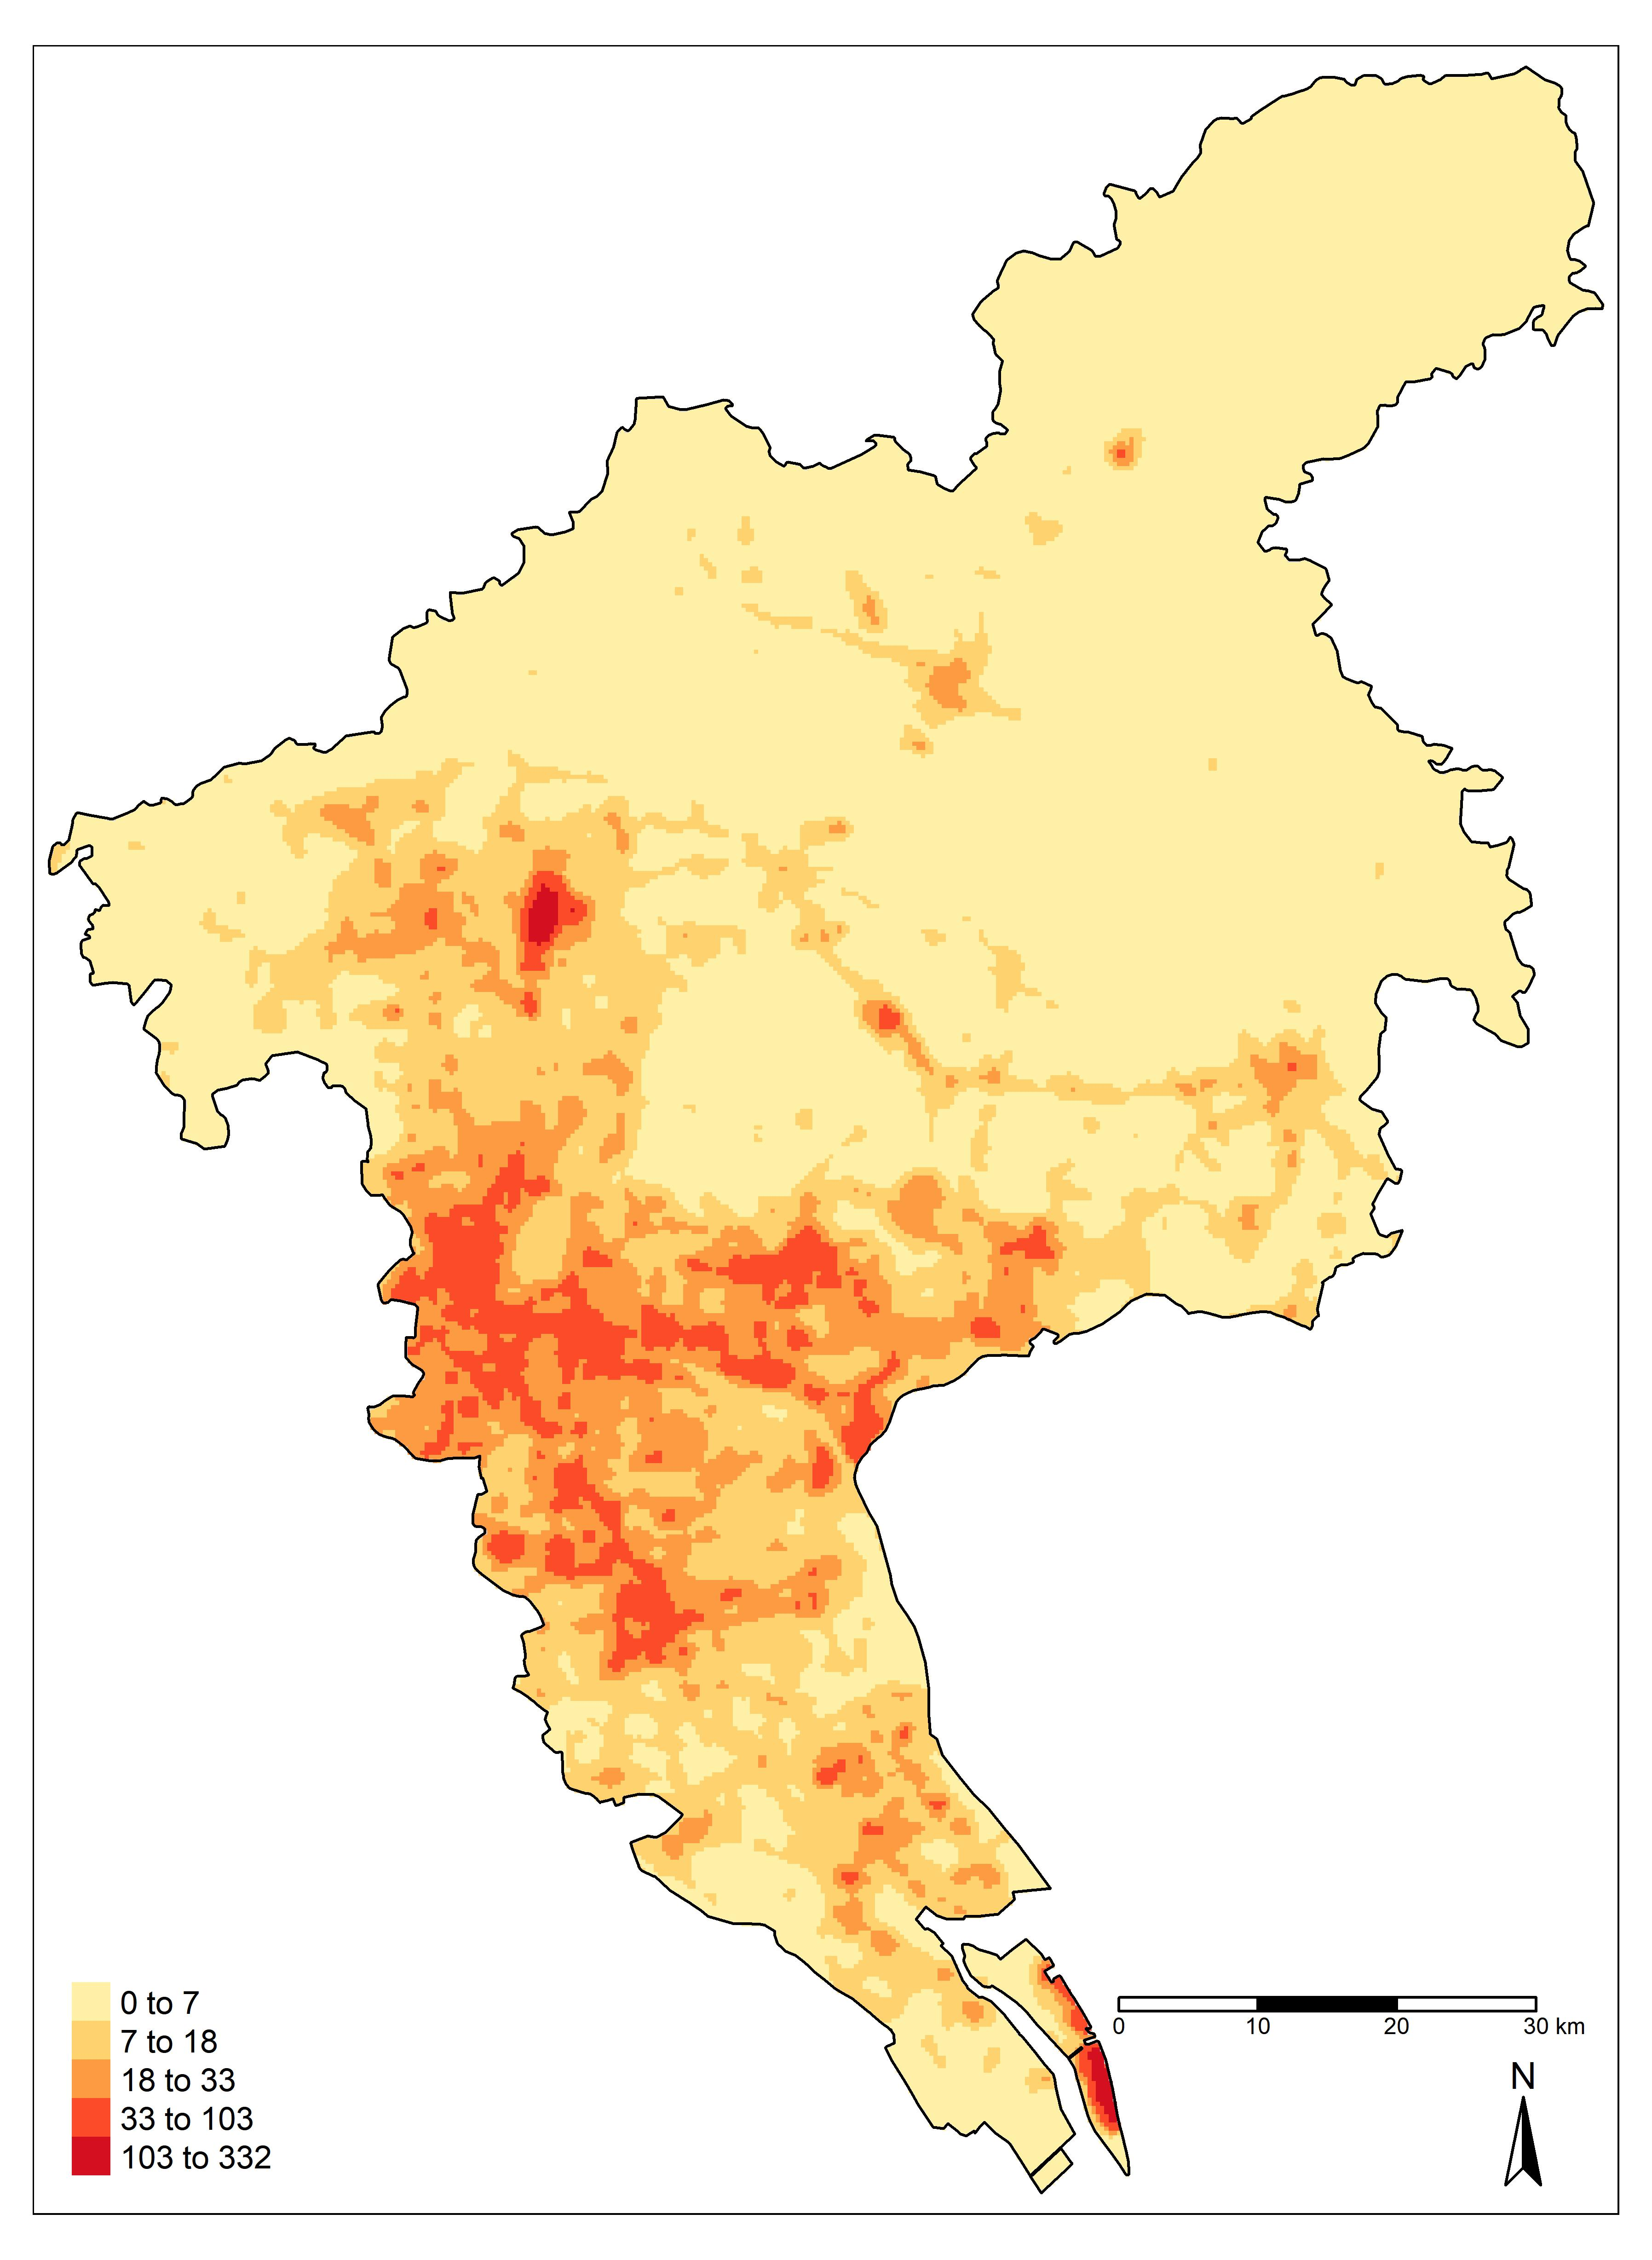
\includegraphics[width=6cm]{Figure/nt_gz.jpg}
}
\caption{Indicators of urban development system in Guangzhou}
\label{ugz}
\end{figure}
%%%%%%%%%%%%%%%%%%%%%%%%%%%%%%%%%%%%

%%%%%%%%%%%%%%%%%%%%%%%%%%%%%%%%%%%%
\begin{figure}[H]
\centering
\subfigure[Socio-economic index]{
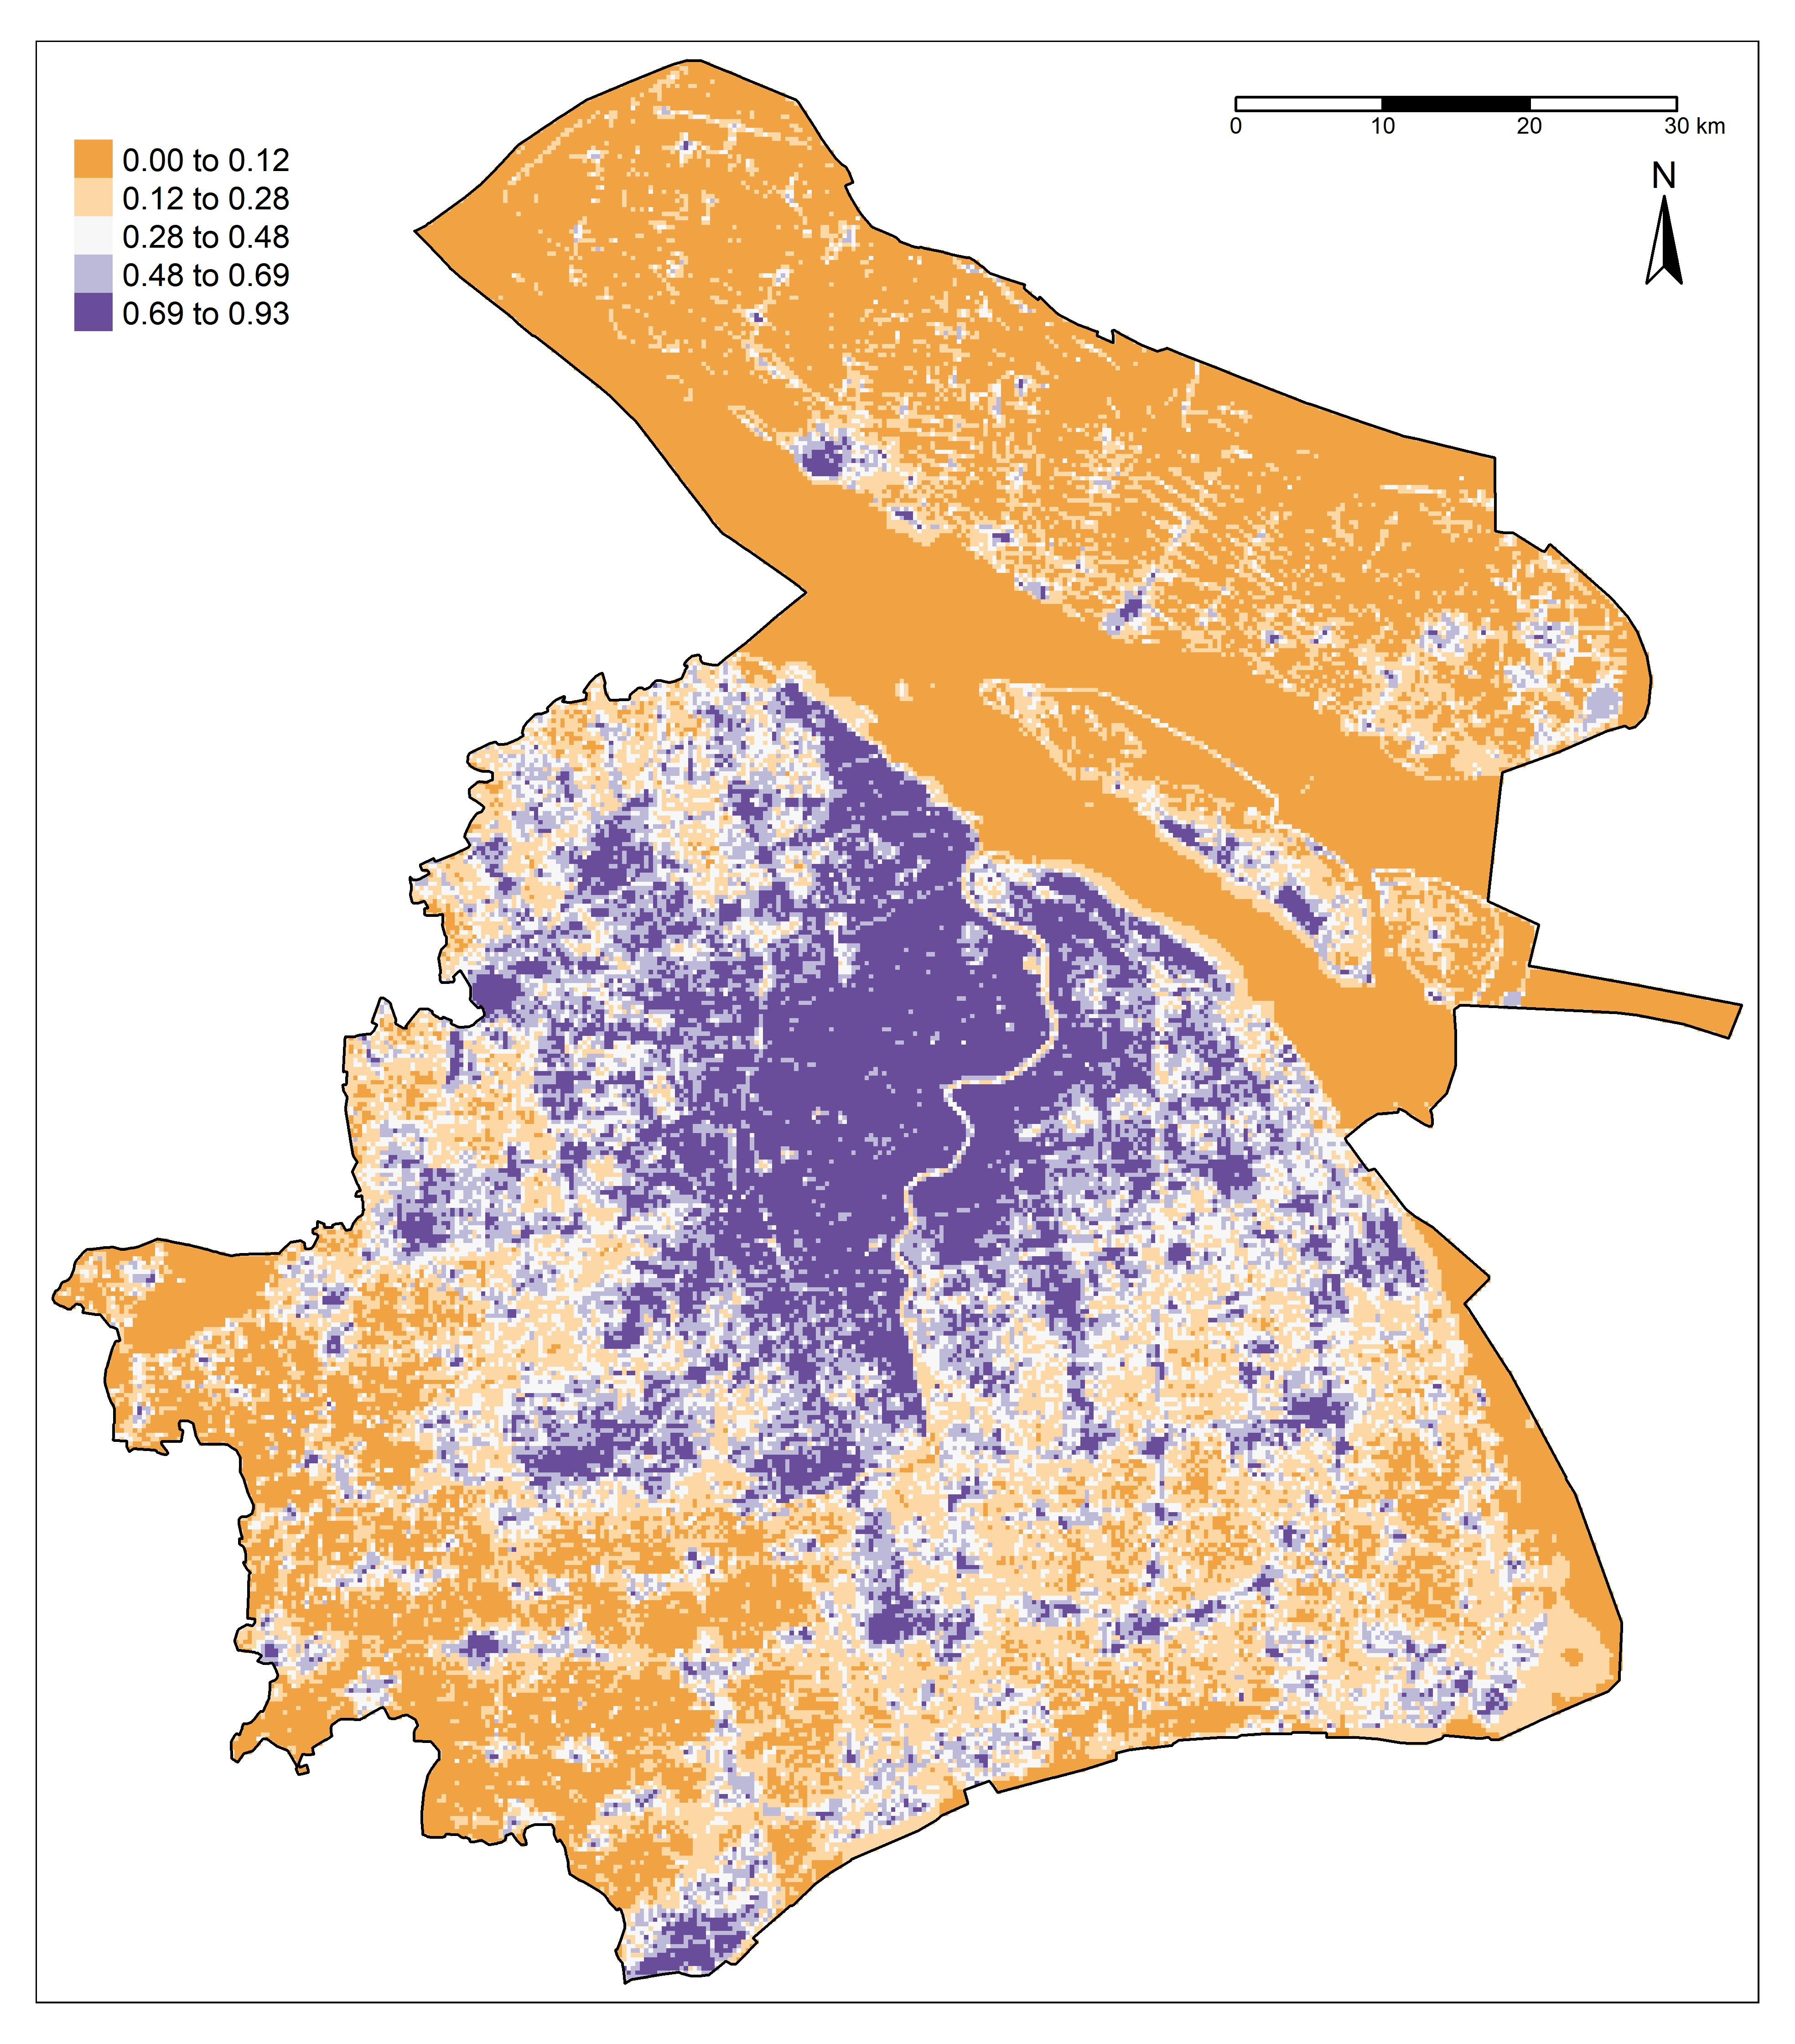
\includegraphics[width=6cm]{Figure/ush.jpg}
}
\quad
\subfigure[AL]{
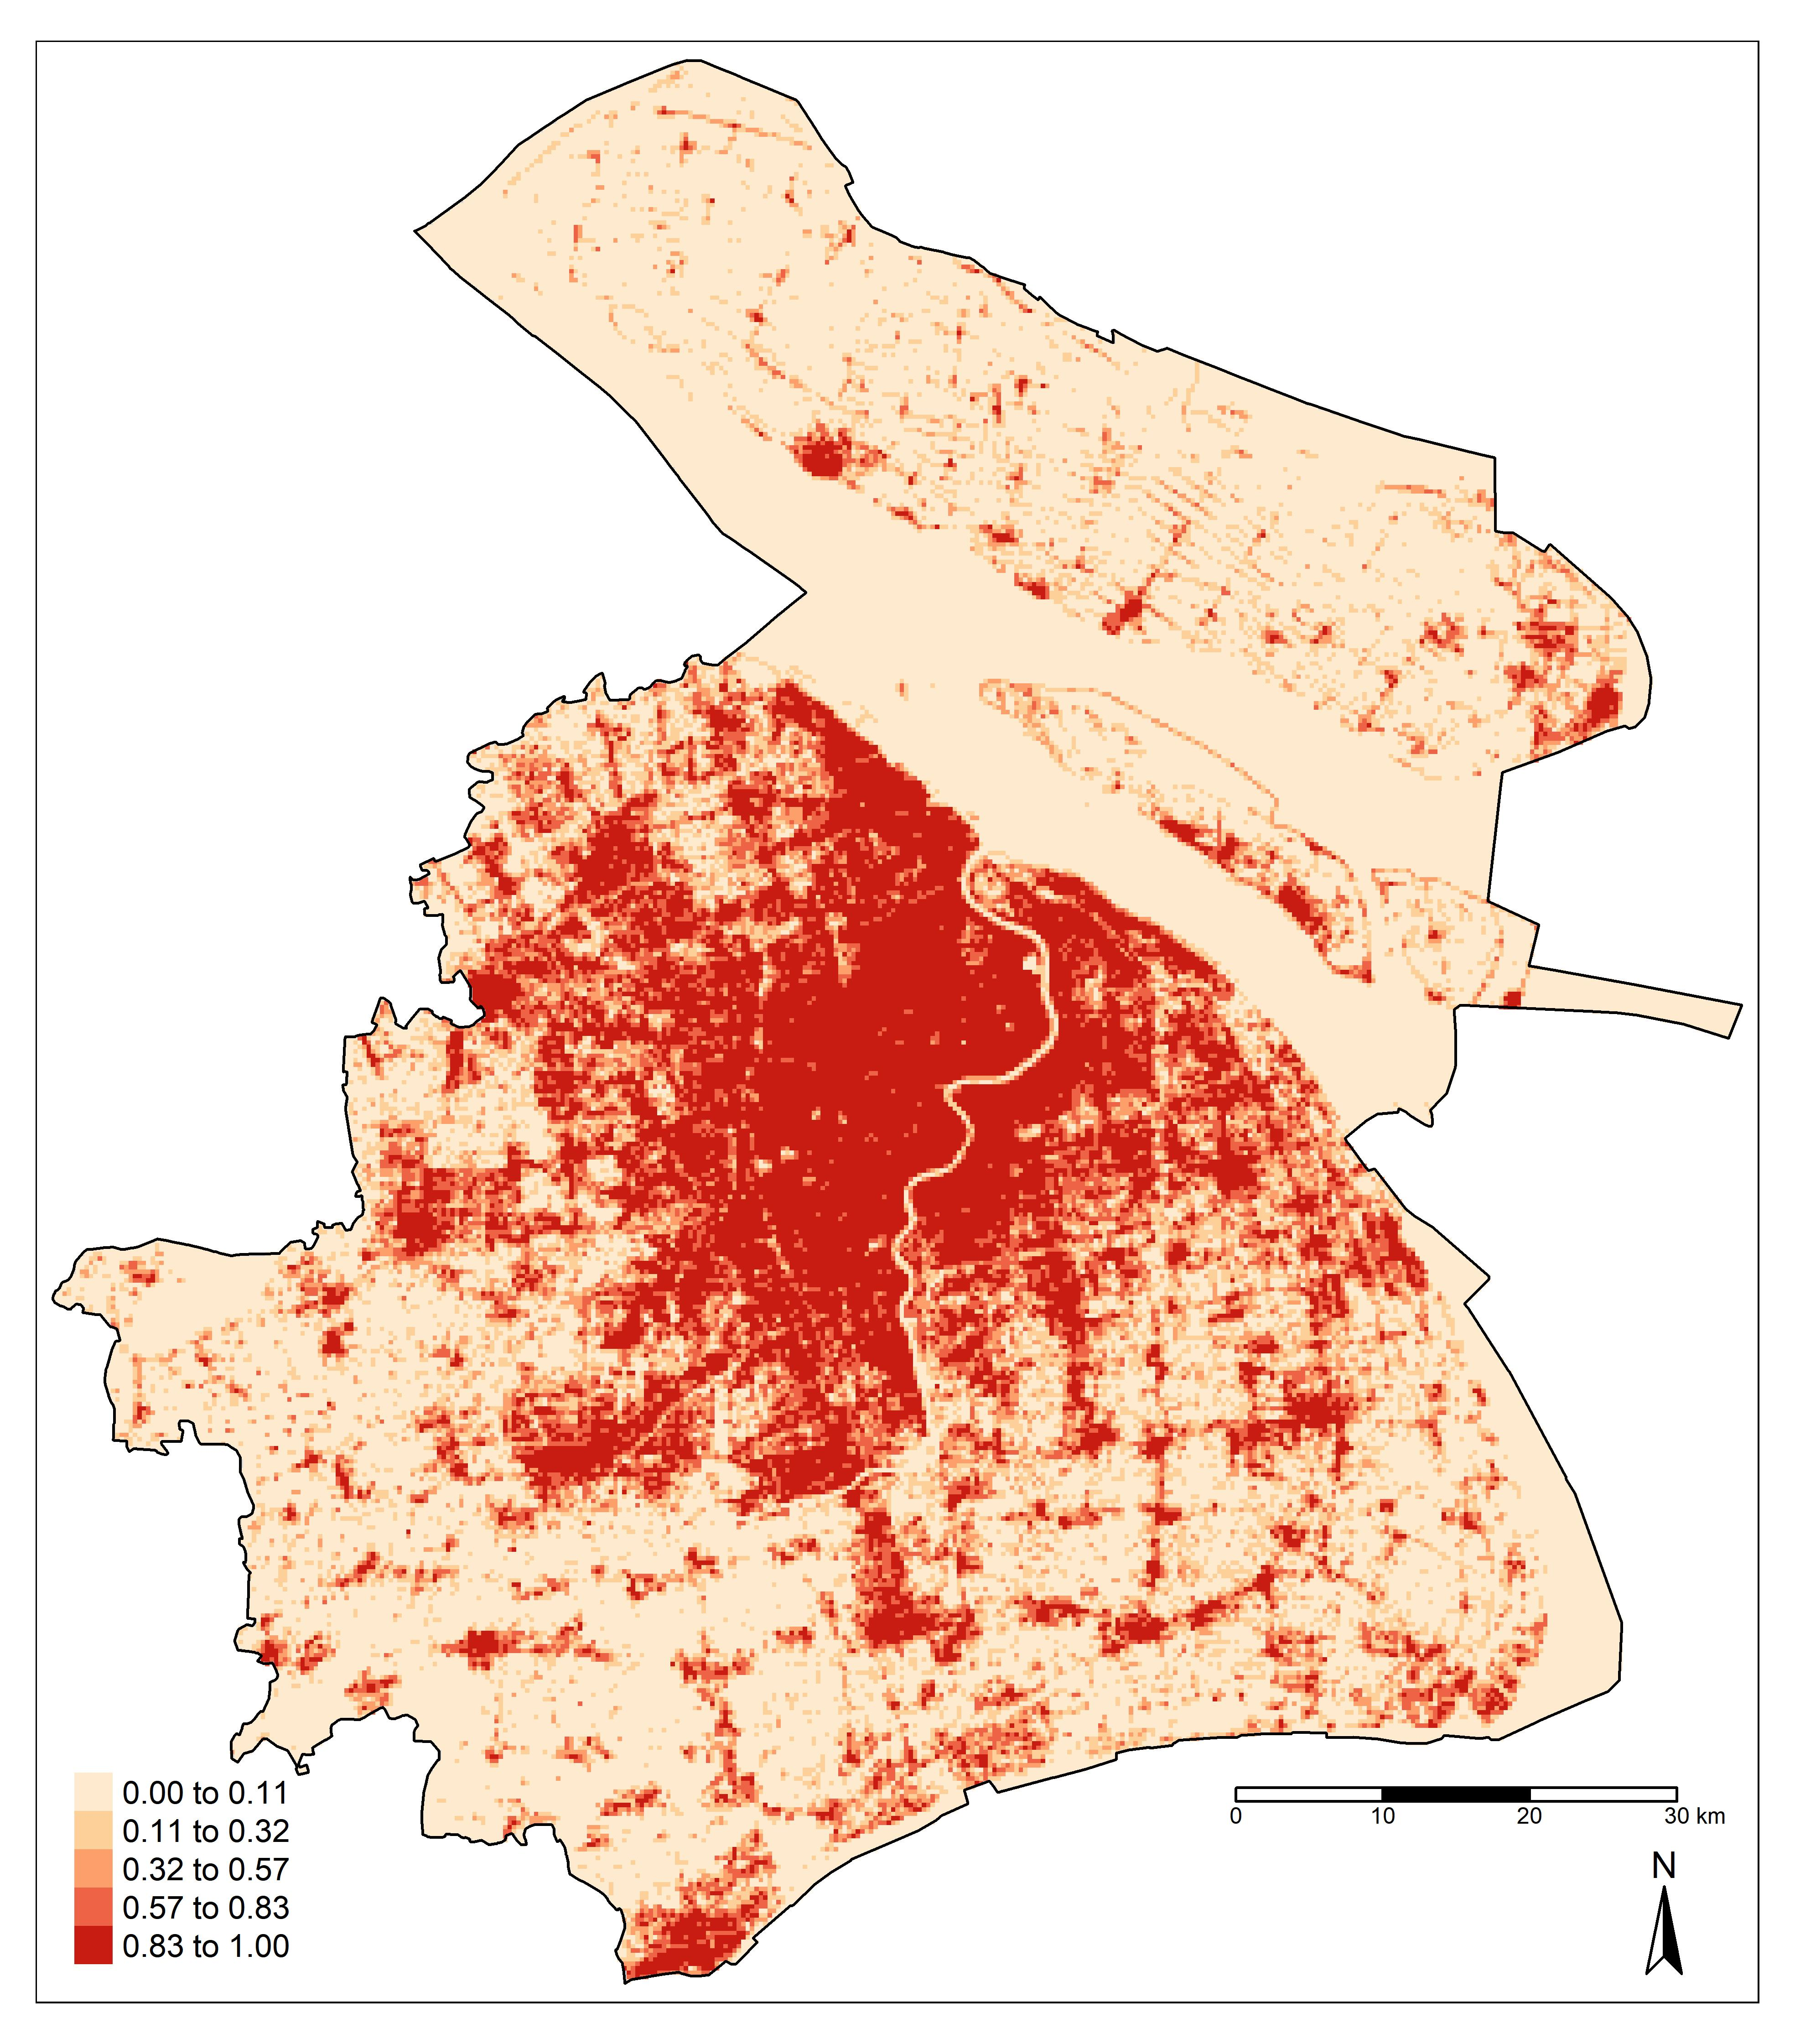
\includegraphics[width=6cm]{Figure/area_sh.jpg}
}
\quad
\subfigure[CL]{
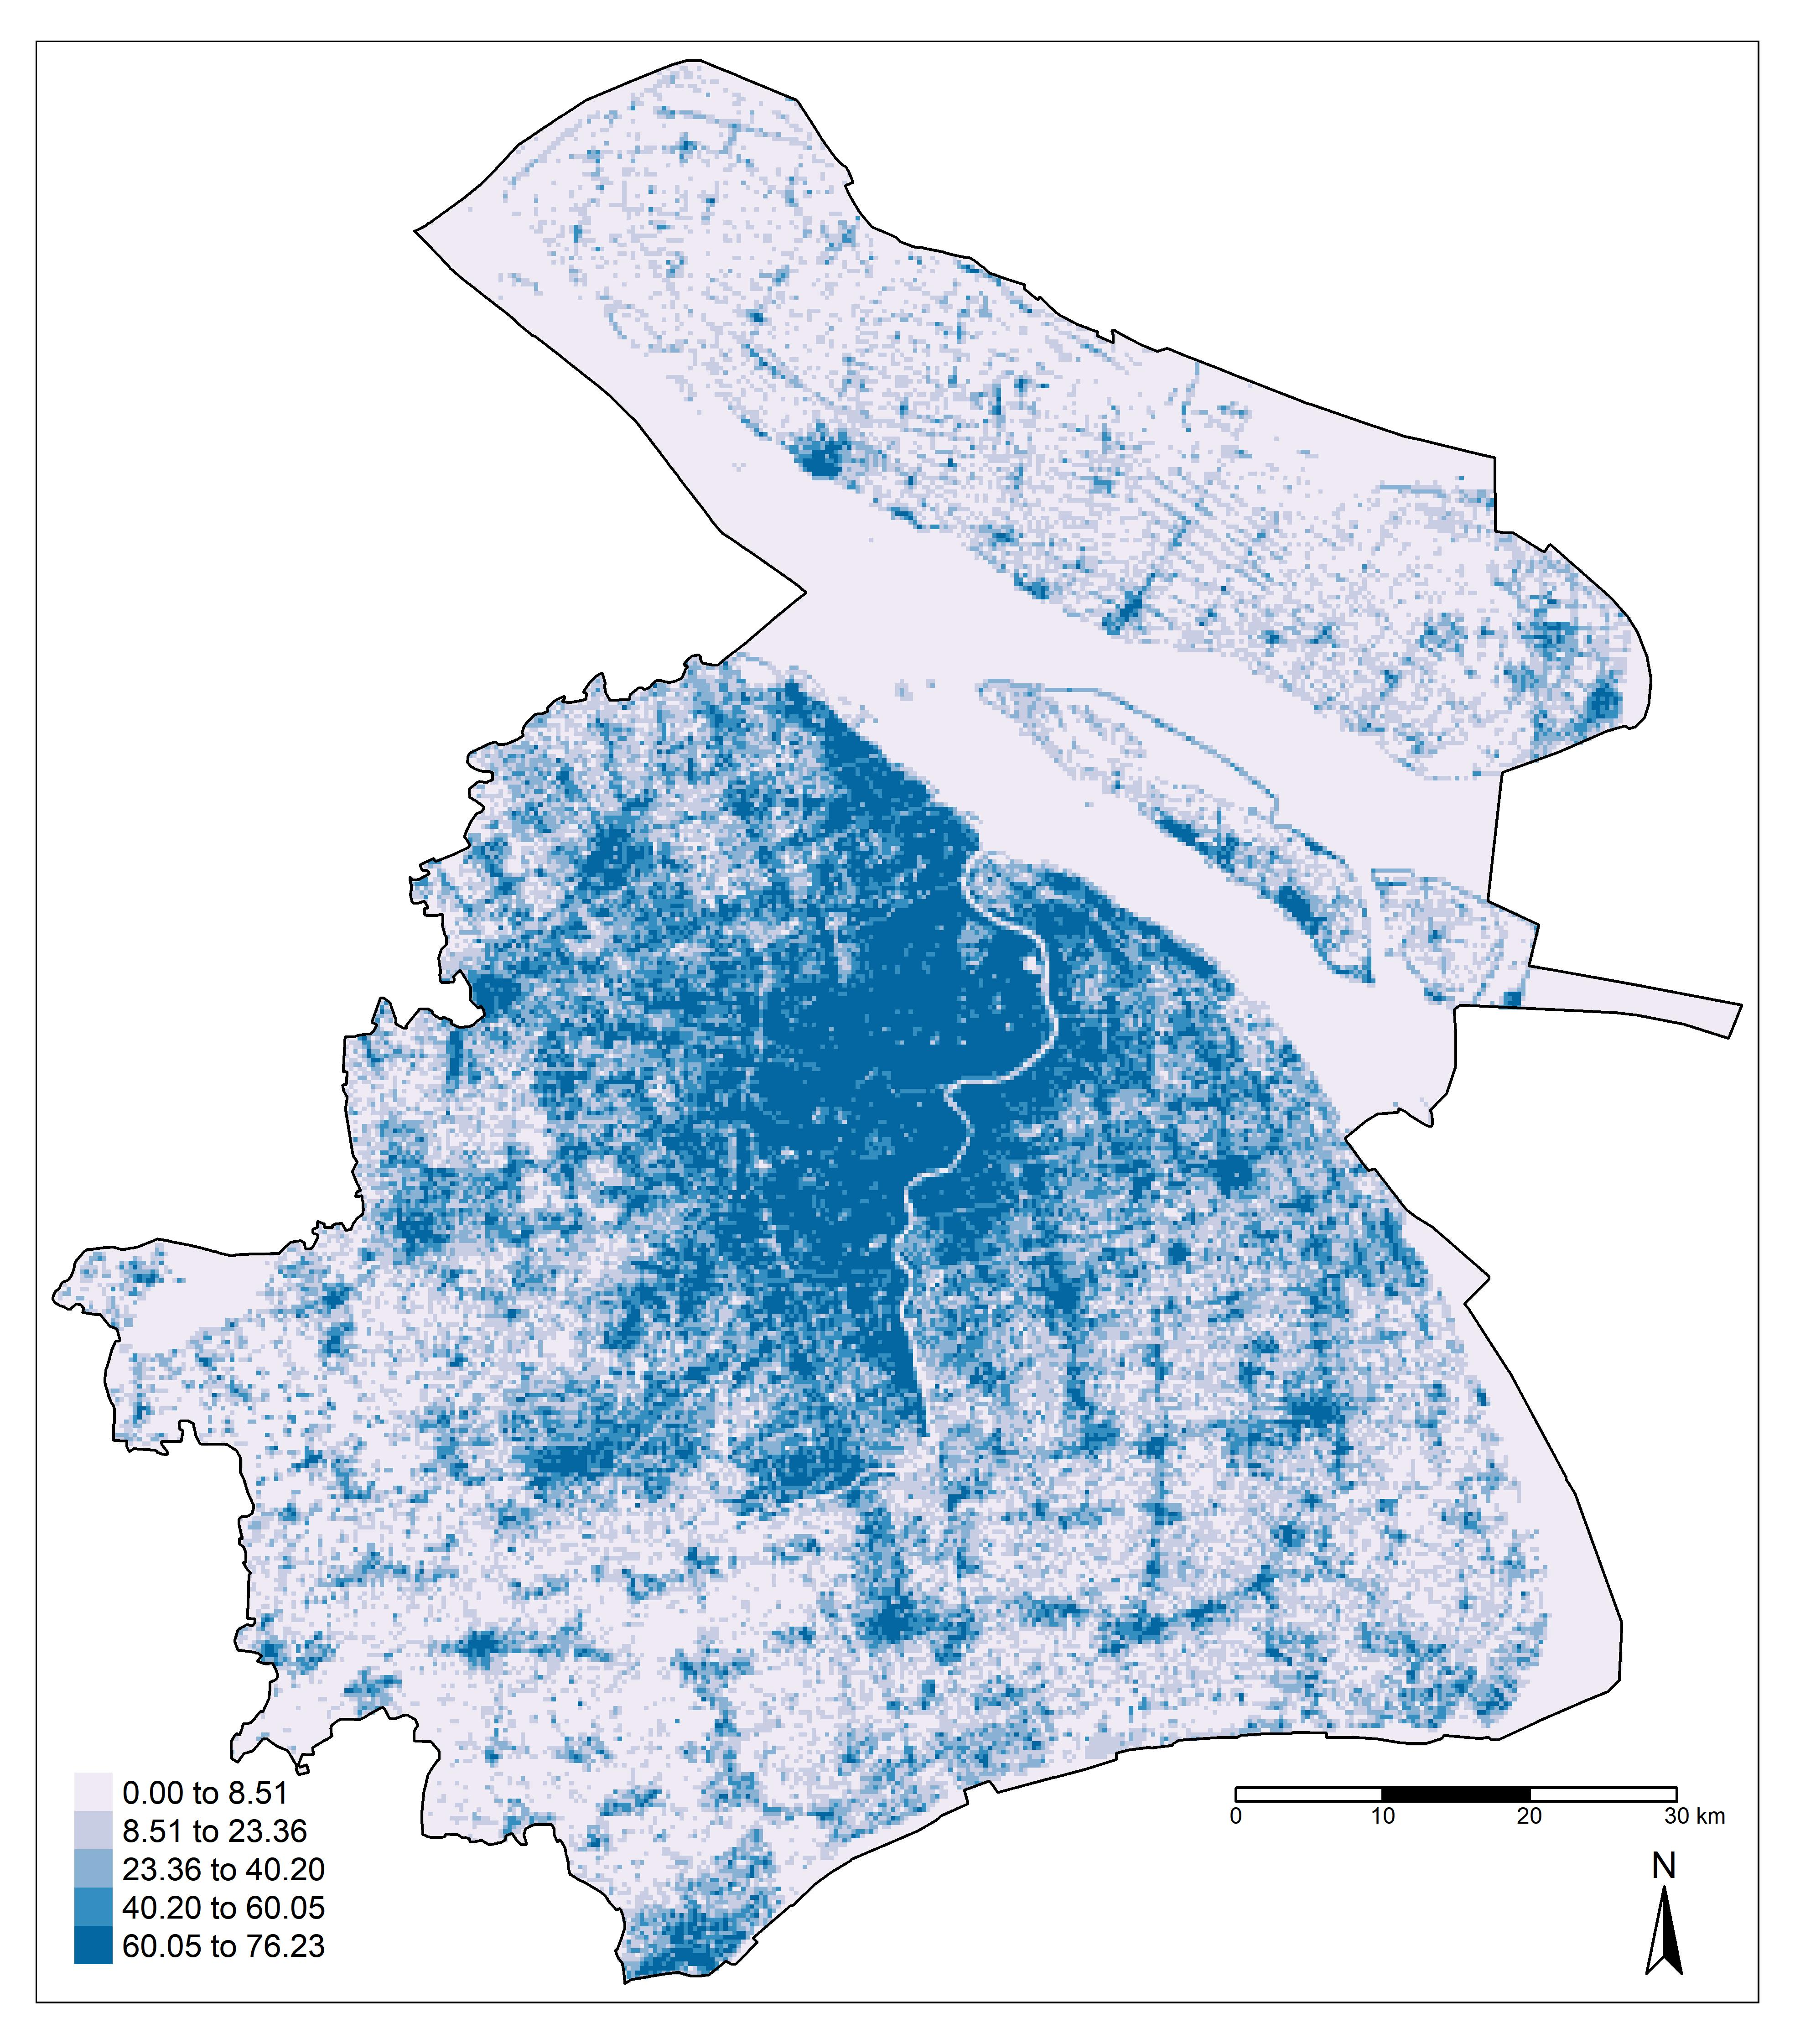
\includegraphics[width=6cm]{Figure/length_sh.jpg}
}
\quad
\subfigure[NT]{
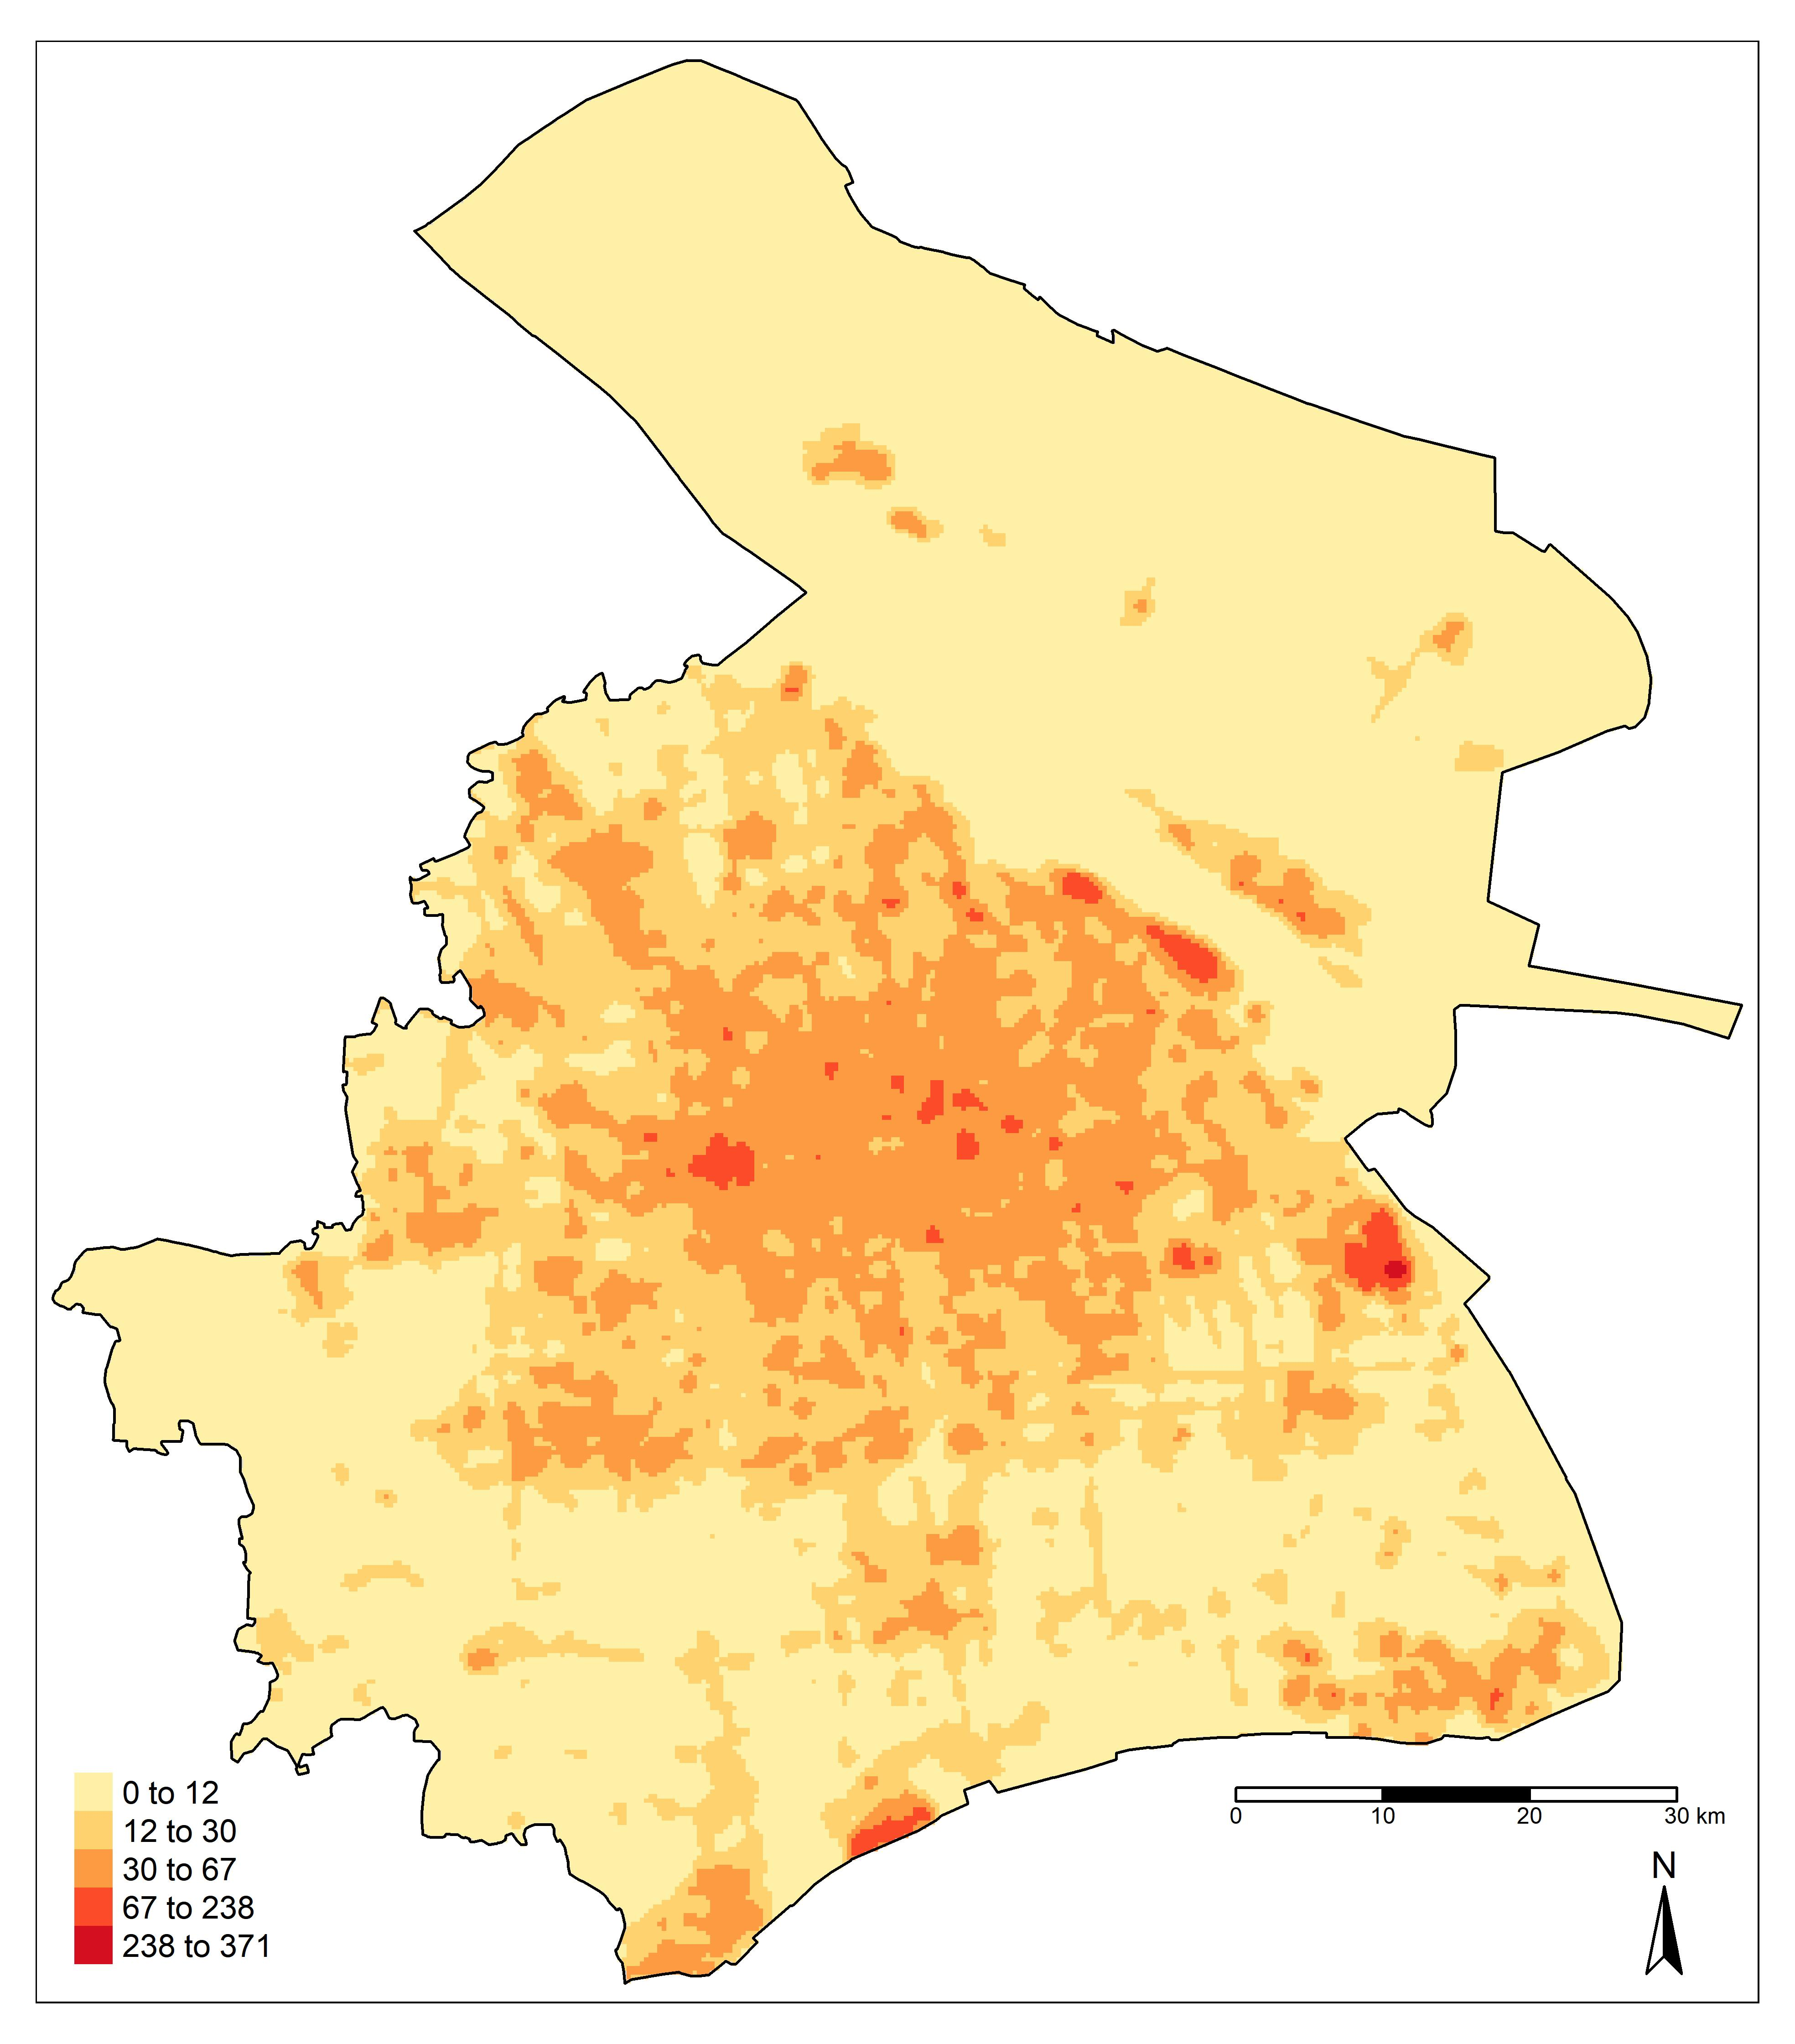
\includegraphics[width=6cm]{Figure/nt_sh.jpg}
}
\caption{Indicators of urban development system in Shanghai}
\label{ush}
\end{figure}
%%%%%%%%%%%%%%%%%%%%%%%%%%%%%%%%%%%%

\subsubsection{Urban development system indicators}
There was a distinctive feature of the NT value. When comparing with the socio-economic index, the area with high NT values were basically the same as index. Besides, NT values were mostly concentrated in the areas of construction land and farmland. In contrast to index, the highest values of NT in Guangzhou were clustered in the central northern area and the southern fringe close to the South China Sea. While the highest values in Shanghai were also partially distributed in the southern border and the eastern area close to the East China Sea. Whereas Guangzhou was compared with Shanghai, the highest value and average value of Shanghai was much larger than Guangzhou, which would further indicate that in the socio-economic development level of the city, Shanghai had a higher degree of urbanization development than Guangzhou.\\

The high-value areas in AL were mostly found in the central and southern part of Guangzhou, and the central and southern part of Shanghai. The high-value areas in AL were mostly found in the central and southern part of Guangzhou and the central and southern part of Shanghai. Compared with NT, the distribution of high-value areas from AL was more concentrated. It can be seen that the NT value remained at a low value in some areas where urban construction land was concentrated. This also showed that there were some differences in the development of construction land when it comes to development level and business potential.\\

There was some similarity between AL and CL. However, compared with AL, CL had a more uniform distribution. Especially in the central south and northwest areas of Guangzhou and the southern area of Shanghai, the high compactness areas were basically in a scattered but uniform distribution.\\



\subsubsection{Environmental index}
According to the figure Figure \ref{egz} and \ref{esh}, The high-values of environmental index in Guangzhou were mainly concentrated in the mountainous and woodland areas in the northern part of the city. In terms of the spatial layout of Guangzhou, some of the areas with the highest values were mostly close to the urban boundary areas. This may be due to the relatively low level of development and fewer traces of human activities in the border areas. Some of the smaller high-value patches were evenly distributed in the central area of the northern part of the city, which also undertook part of the energy transfer function of the ecological source sites in the northern area. This phenomenon also maintained a stable ecological function in the north side.\\

The index values in the southern part of the city were generally in the medium level. The distribution of high-value areas in the area was more fragmented and there was not a concentrated cluster of patches. This may be due to the relatively low environmental outcome caused by the southward expansion of the city. At the same time, the interspersed distribution of urban construction land led to the fragmentation of large ecological patches.\\

Moreover, The lowest index values were found in the middle of the city. This could also be attributed to the relatively high degree of urban construction in the area. The ecological index of the urban area was also significantly lower.\\

When it comes to Shanghai, there were significant differences between the urban construction land and the non-urban construction areas of the environmental index. In terms of the spatial layout of the area in Shanghai, the index value of construction land in the middle of the city was relatively low. However, the distribution of high-value areas in the surrounding areas of the city was uniformly distributed. There was no uniform concentration of large patches in this type of area, but the high-value areas were evenly interspersed into the medium and low-value areas. This also formed an external ecological network.\\

Compared with Guangzhou, the spatial layout of Shanghai was significantly different. The ecological high-value areas in Guangzhou were concentrated and distributed, while the ecological high-value areas in Shanghai were evenly interspersed.\\

%%%%%%%%%%%%%%%%%%%%%%%%%%%%%%%%%%%%
\begin{figure}[H]
\centering
\subfigure[Environmental index]{
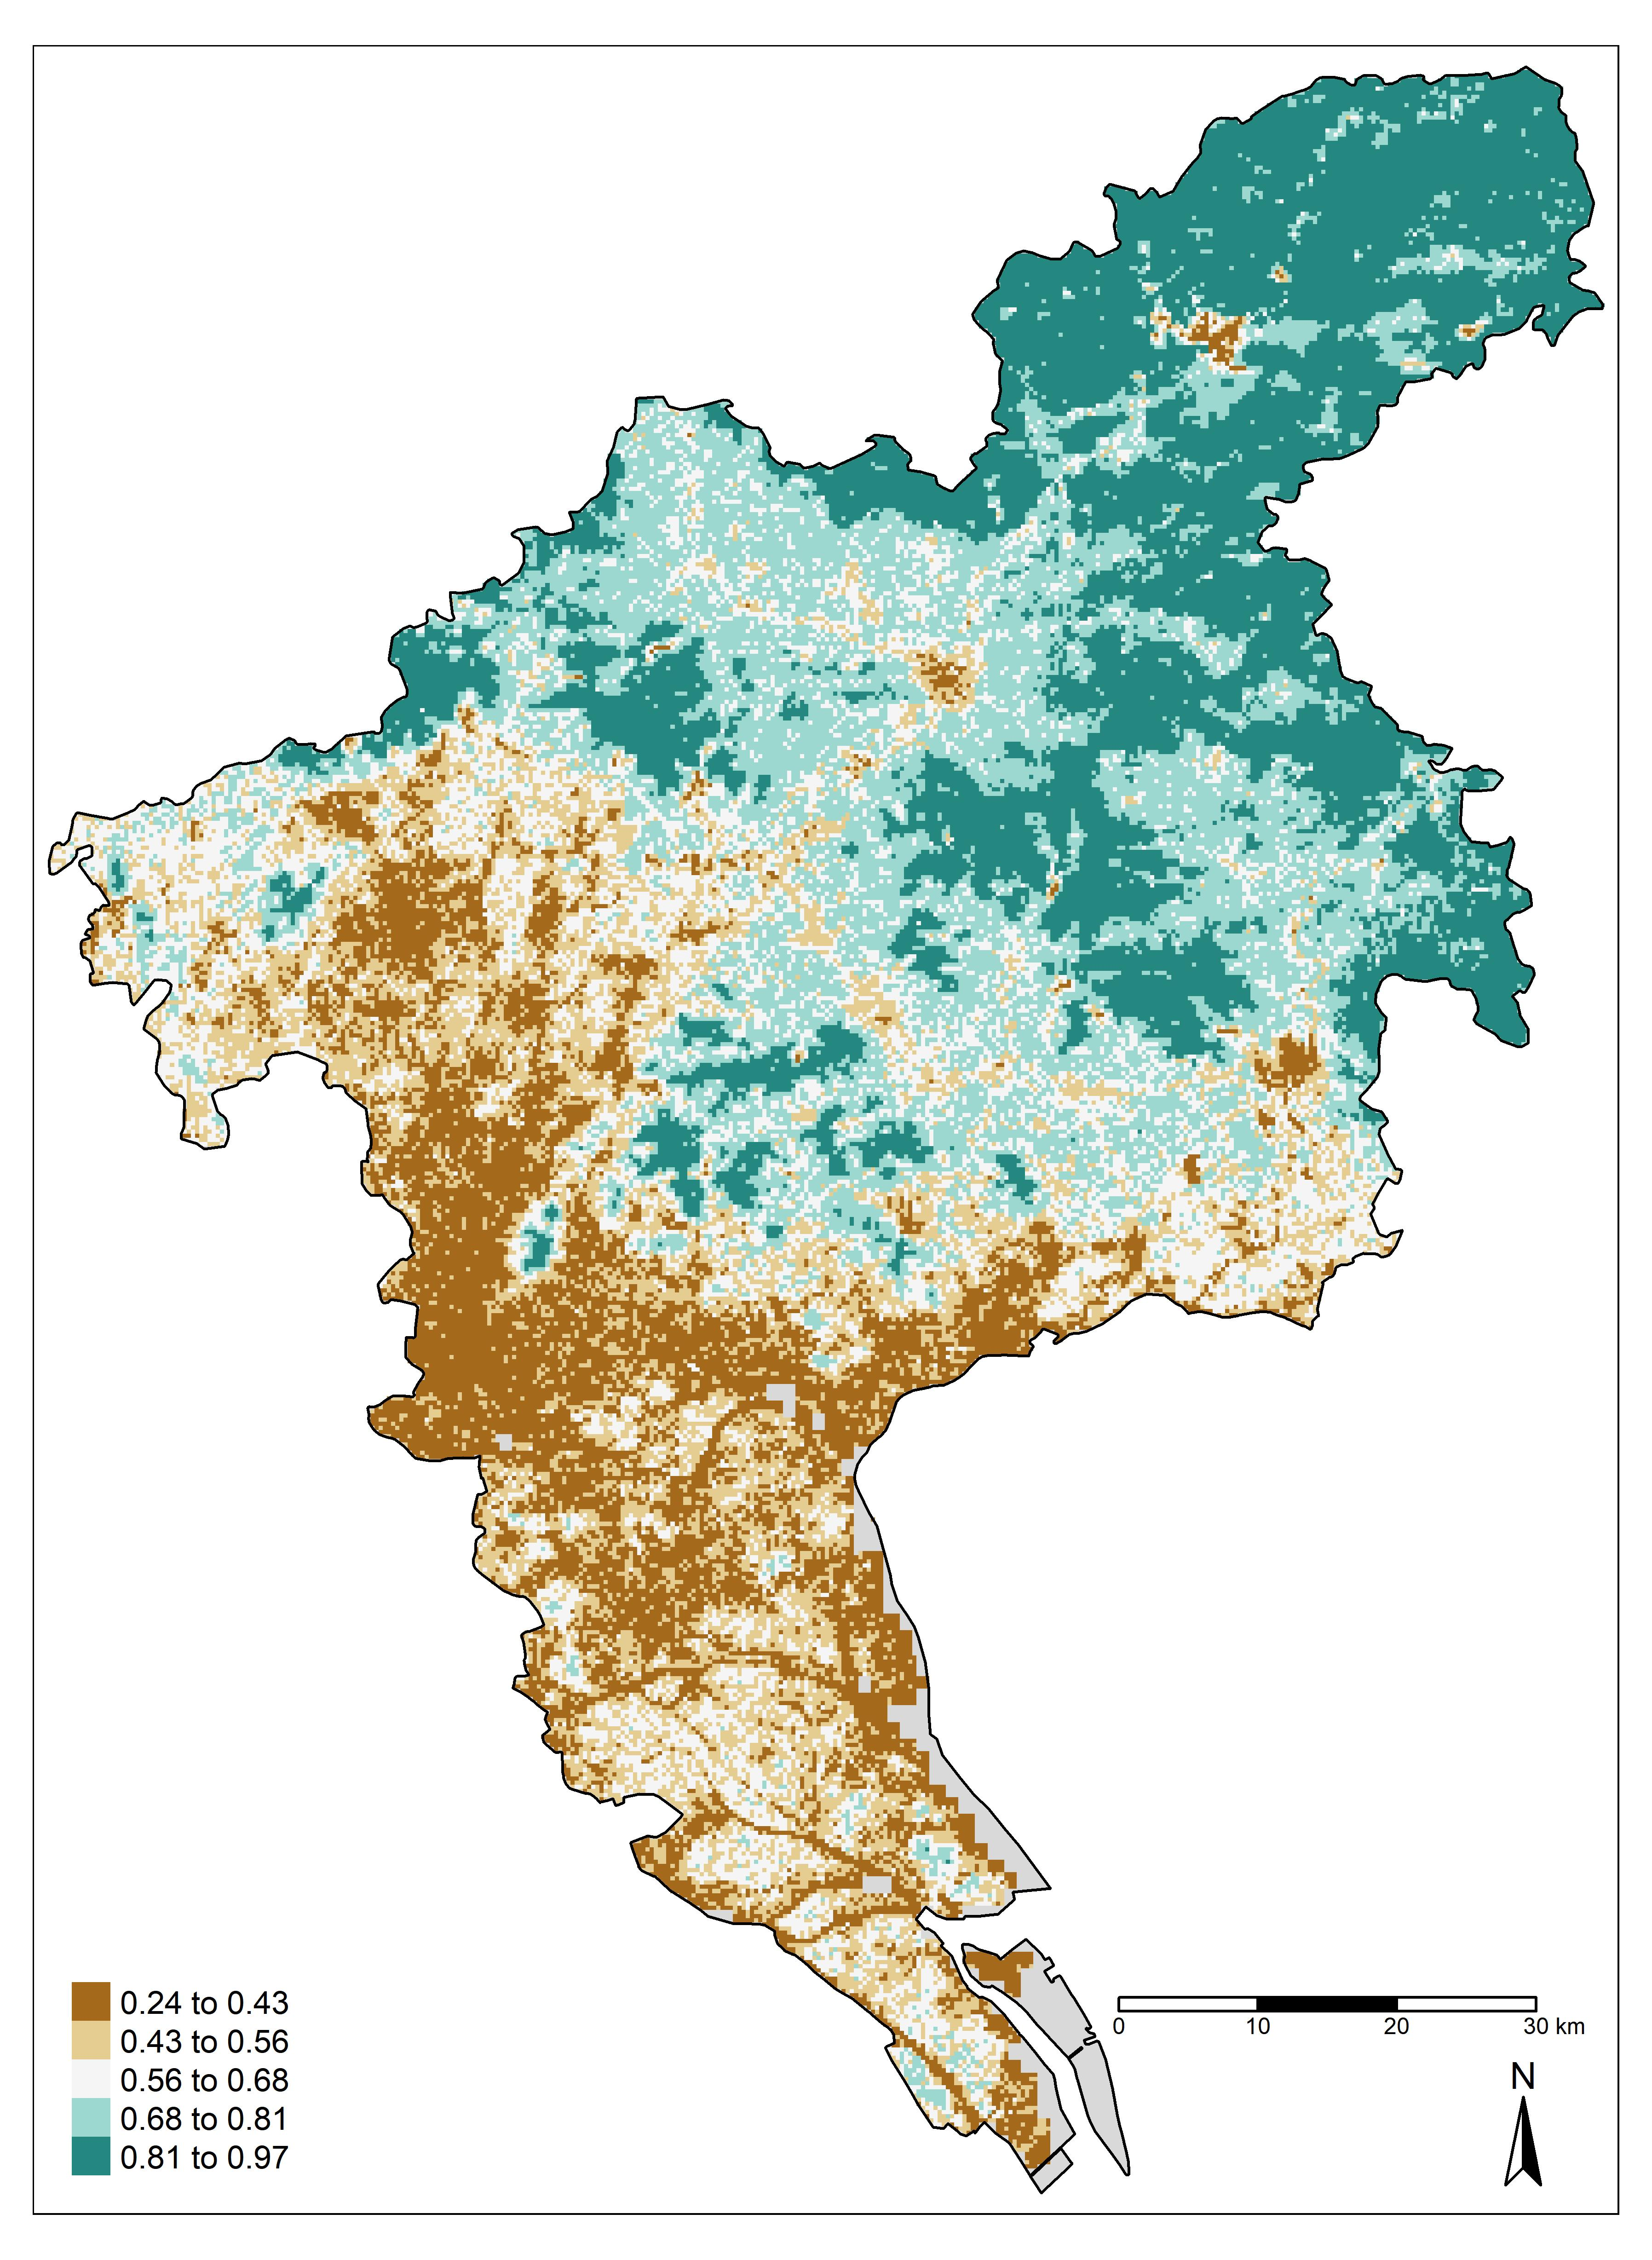
\includegraphics[width=6cm]{Figure/egz.jpg}
}
\quad
\subfigure[NDVI]{
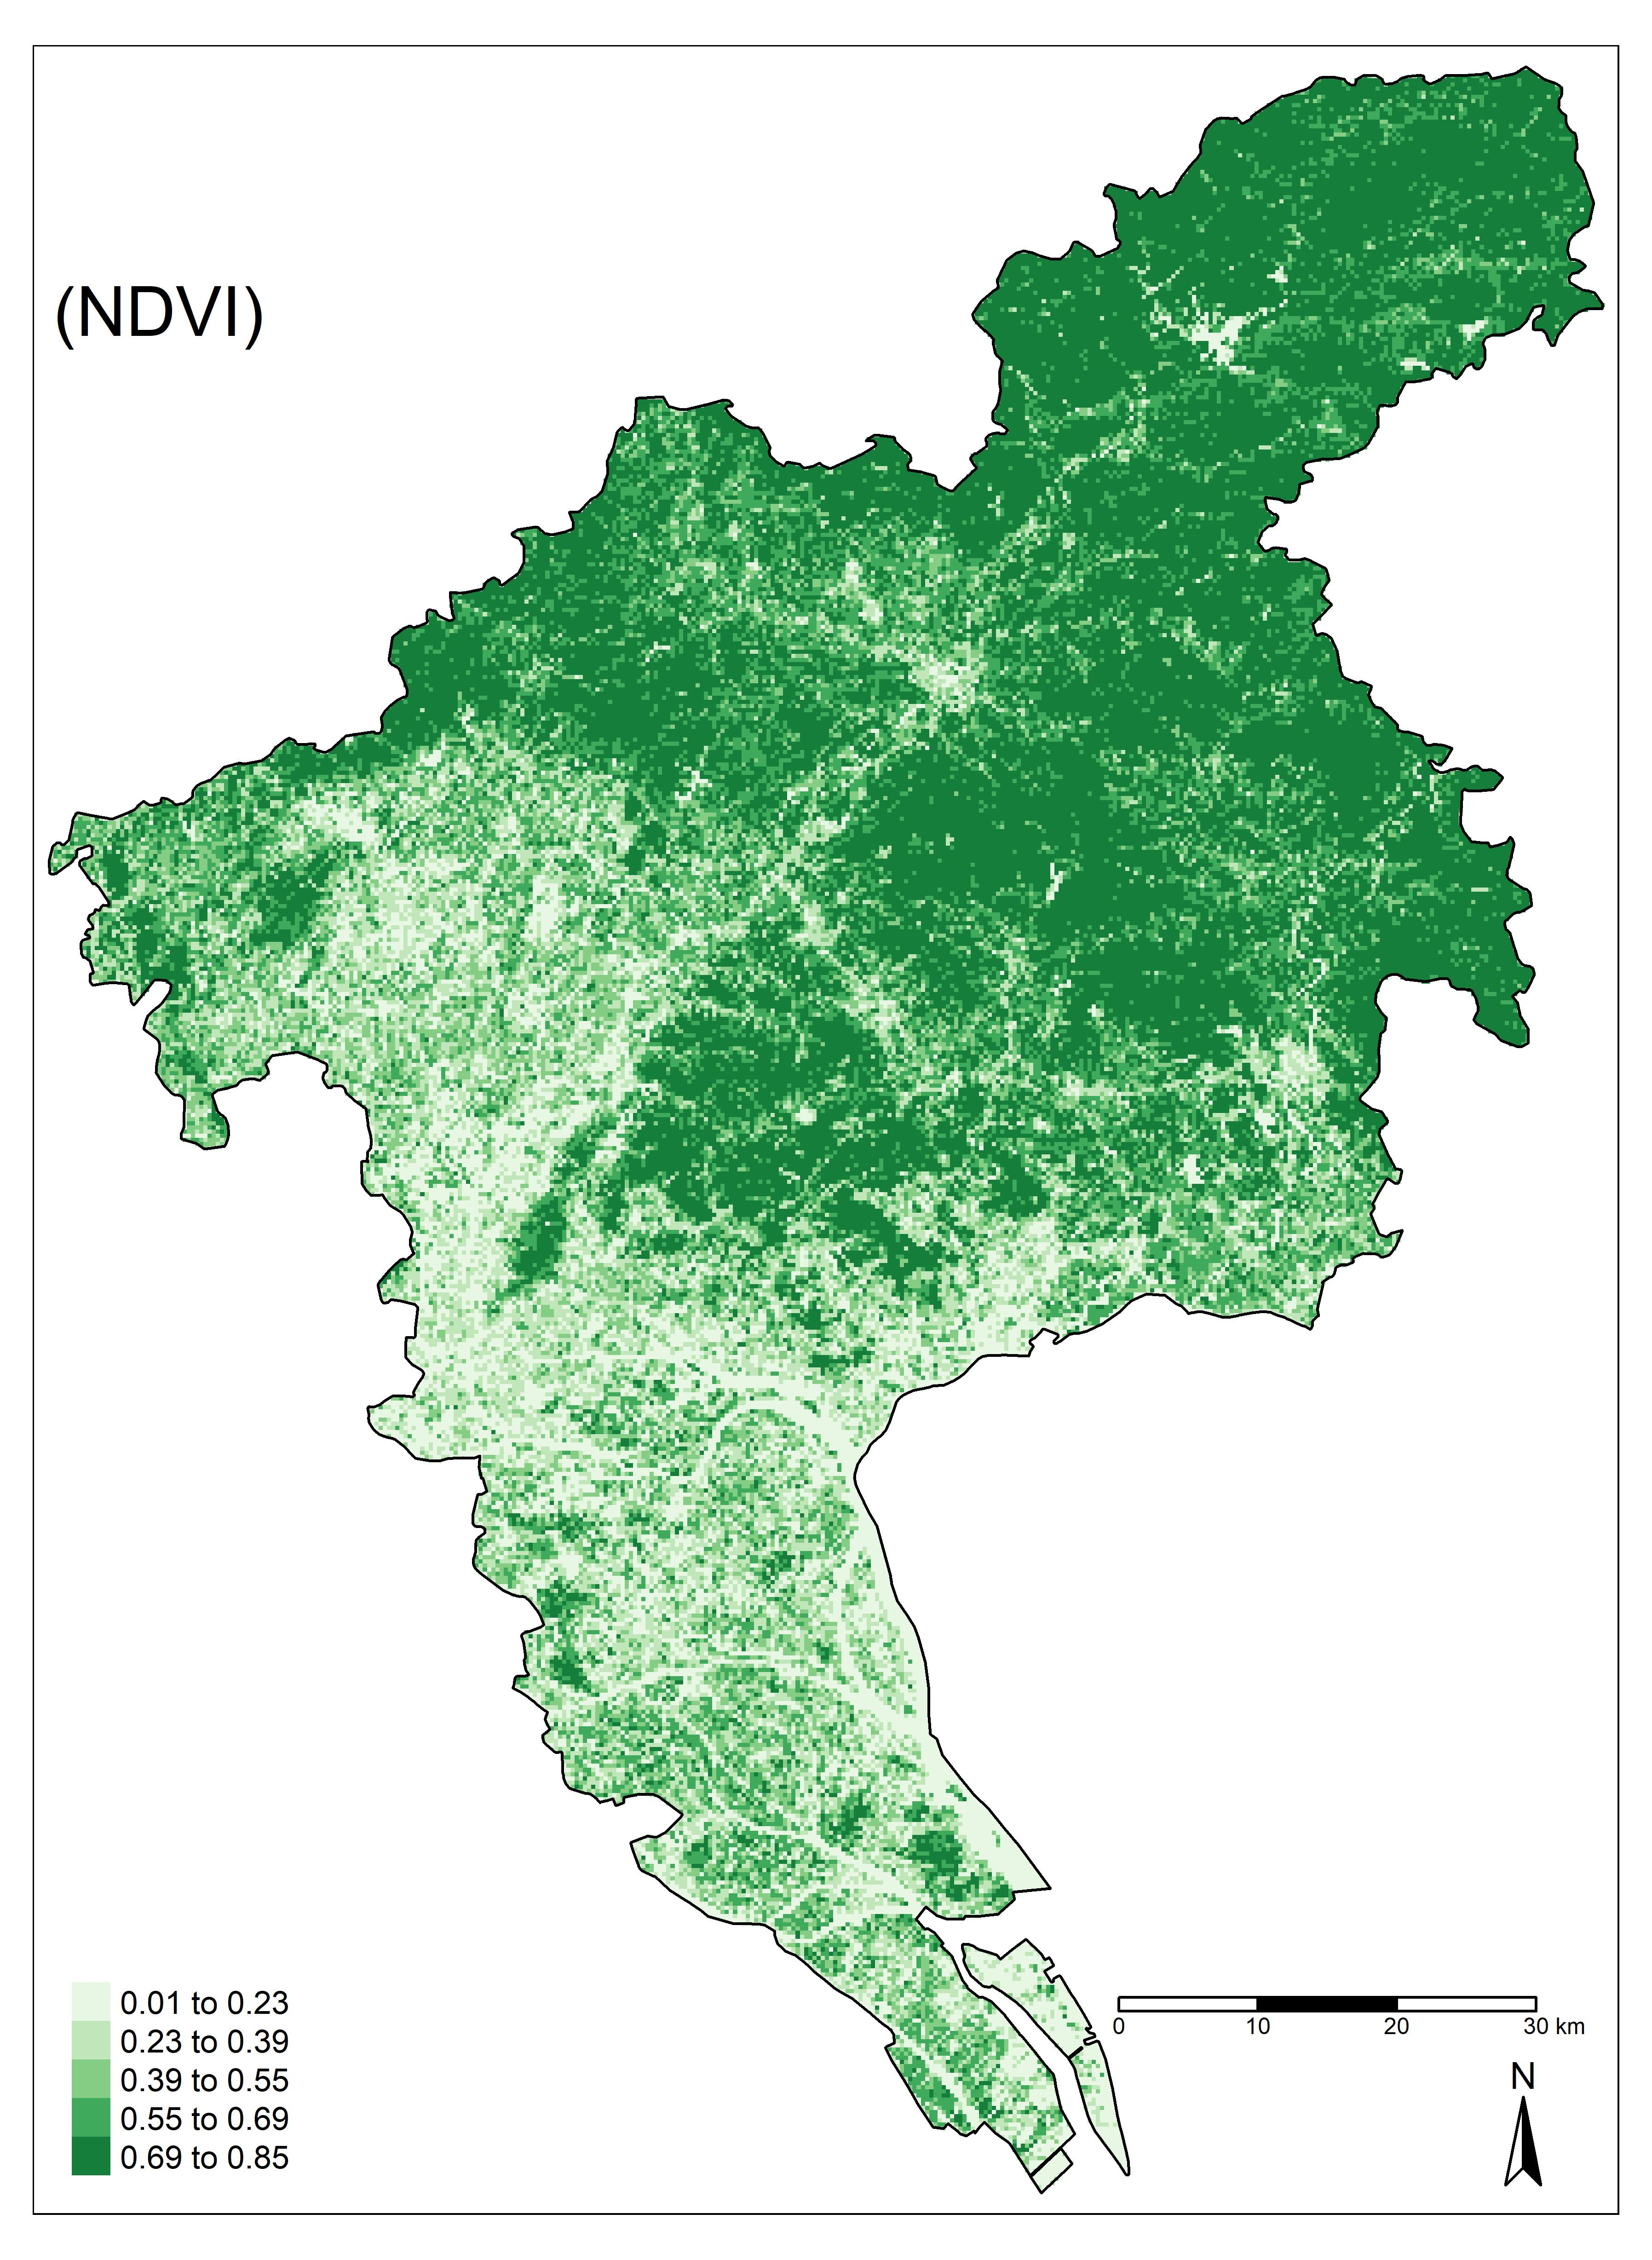
\includegraphics[width=6cm]{Figure/ndvi_gz.jpg}
}
\quad
\subfigure[NPP]{
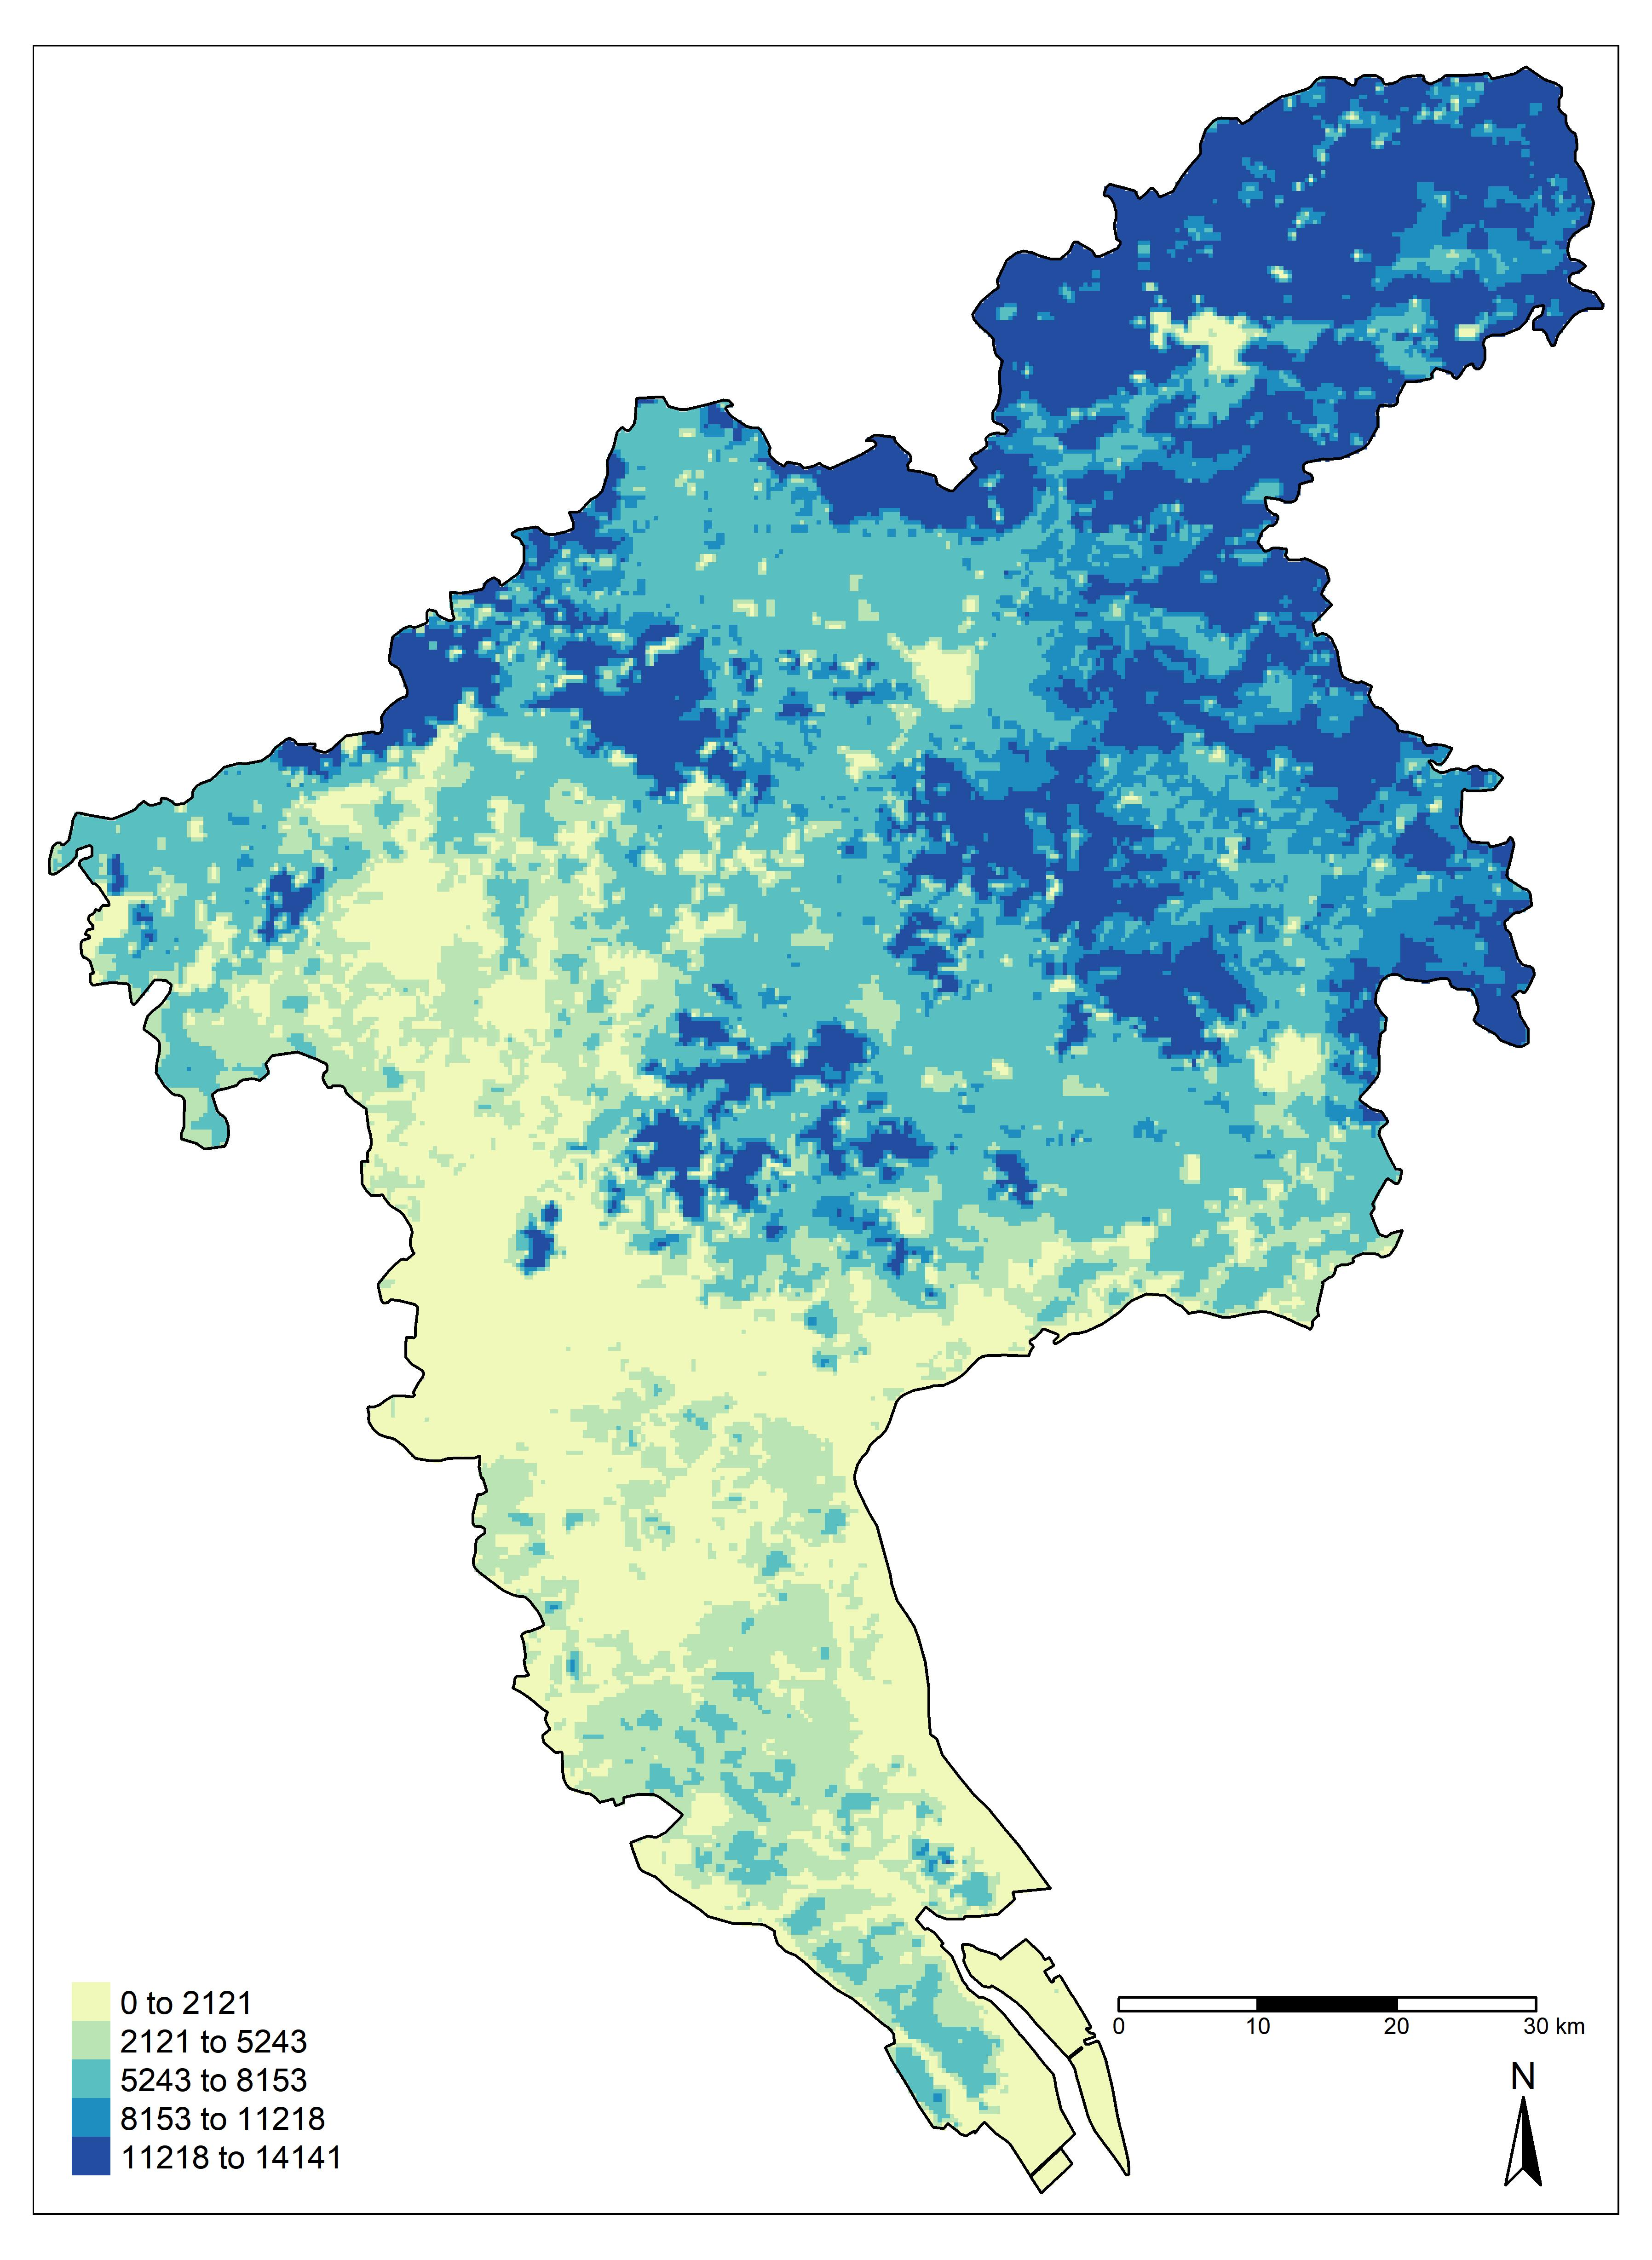
\includegraphics[width=6cm]{Figure/npp_gz.jpg}
}
\quad
\subfigure[PM2.5]{
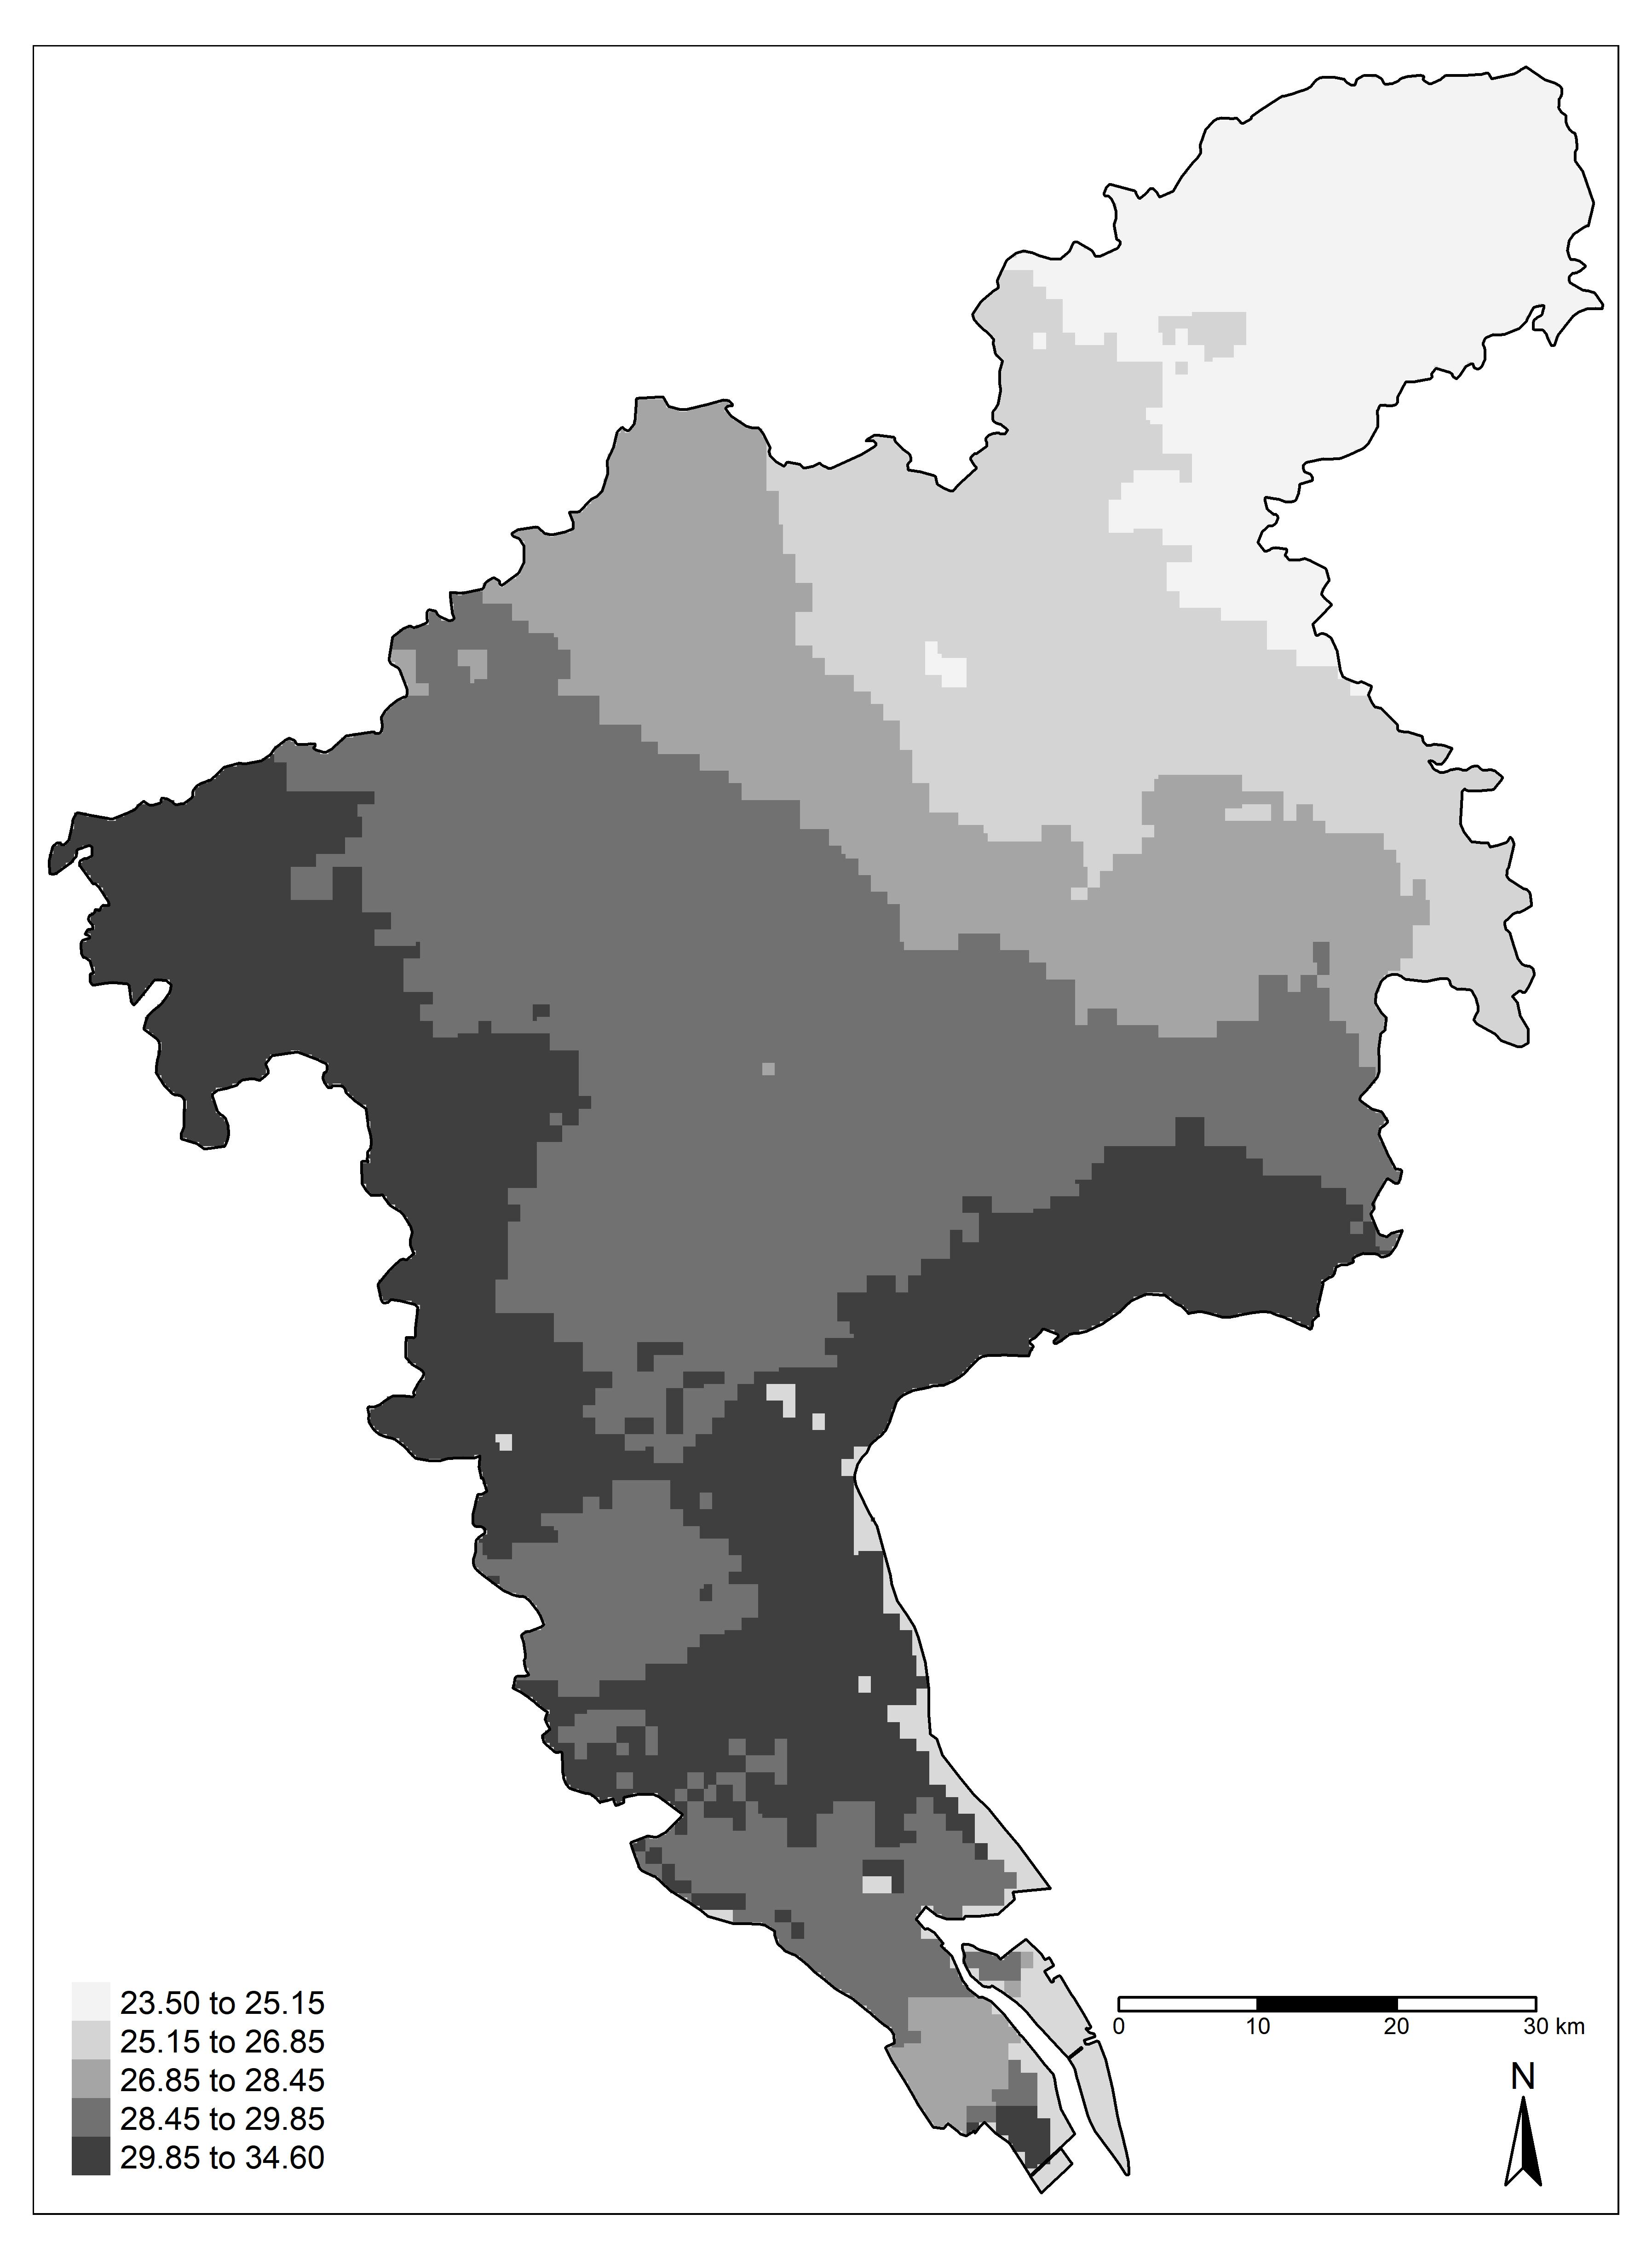
\includegraphics[width=6cm]{Figure/pm_gz.jpg}
}
\caption{Indicators of environmental system in Guangzhou}
\label{egz}
\end{figure}
%%%%%%%%%%%%%%%%%%%%%%%%%%%%%%%%%%%%

%%%%%%%%%%%%%%%%%%%%%%%%%%%%%%%%%%%%
\begin{figure}[H]
\centering
\subfigure[Environmental index]{
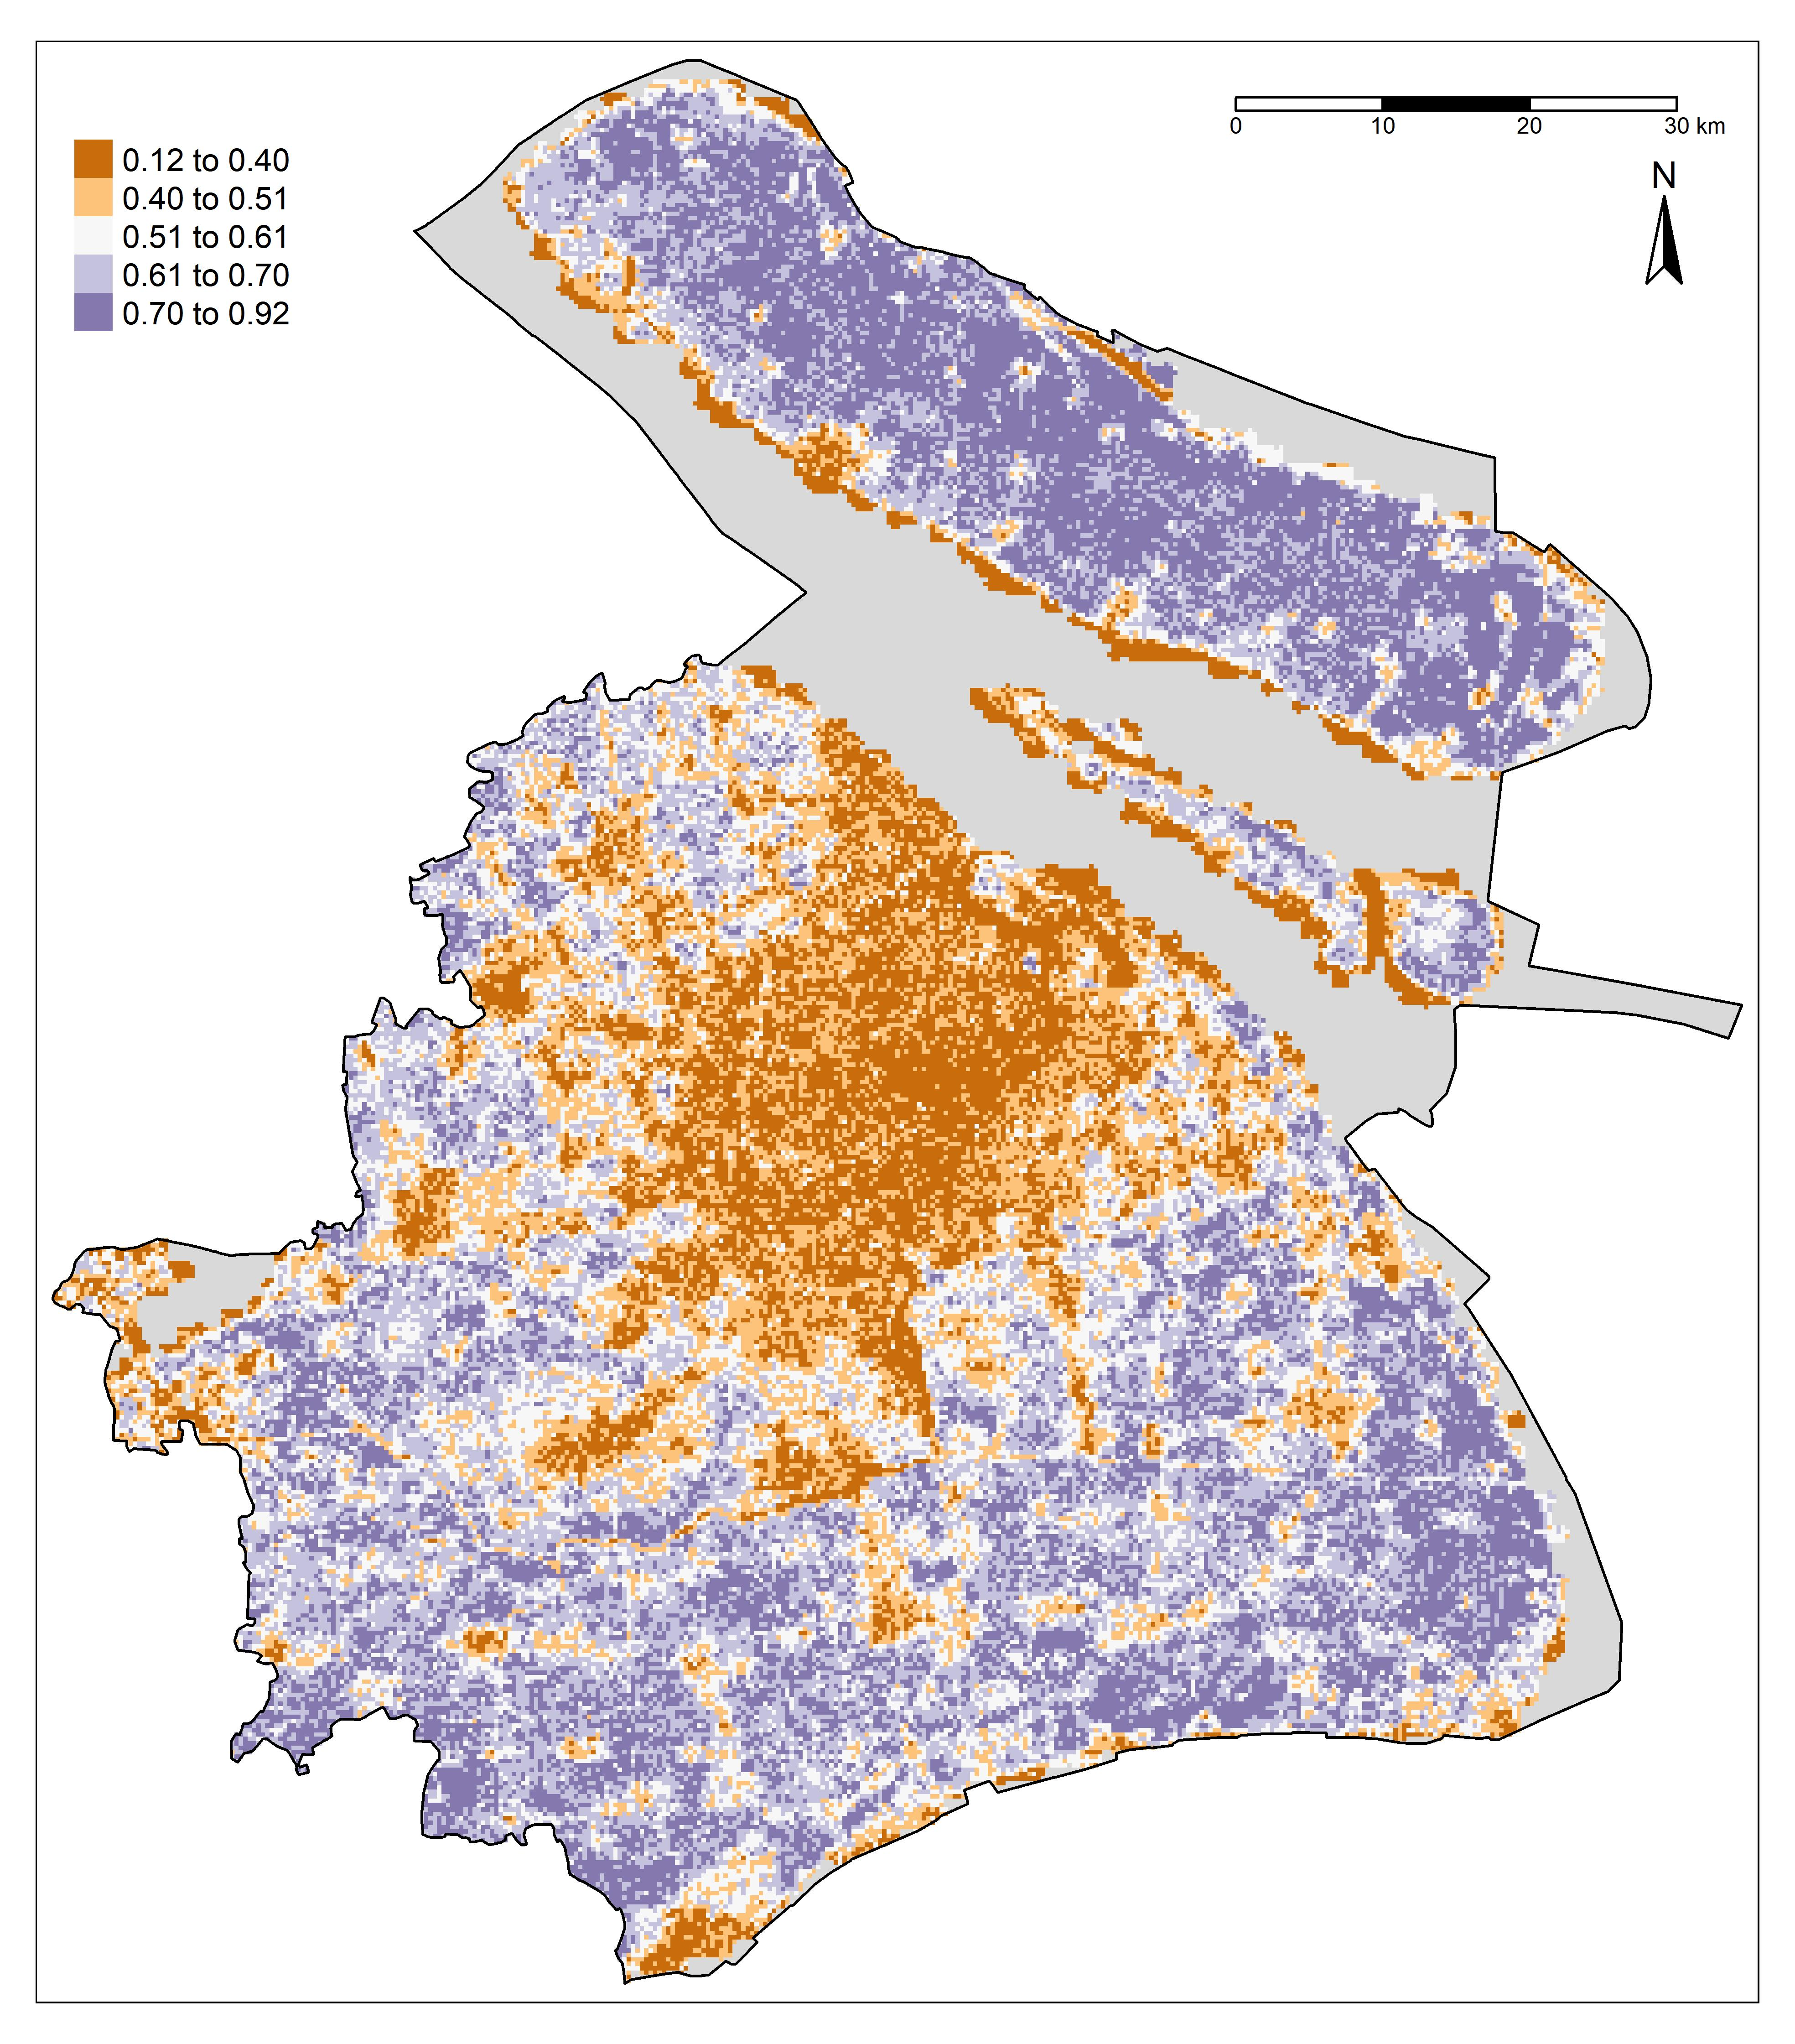
\includegraphics[width=6cm]{Figure/esh.jpg}
}
\quad
\subfigure[NDVI]{
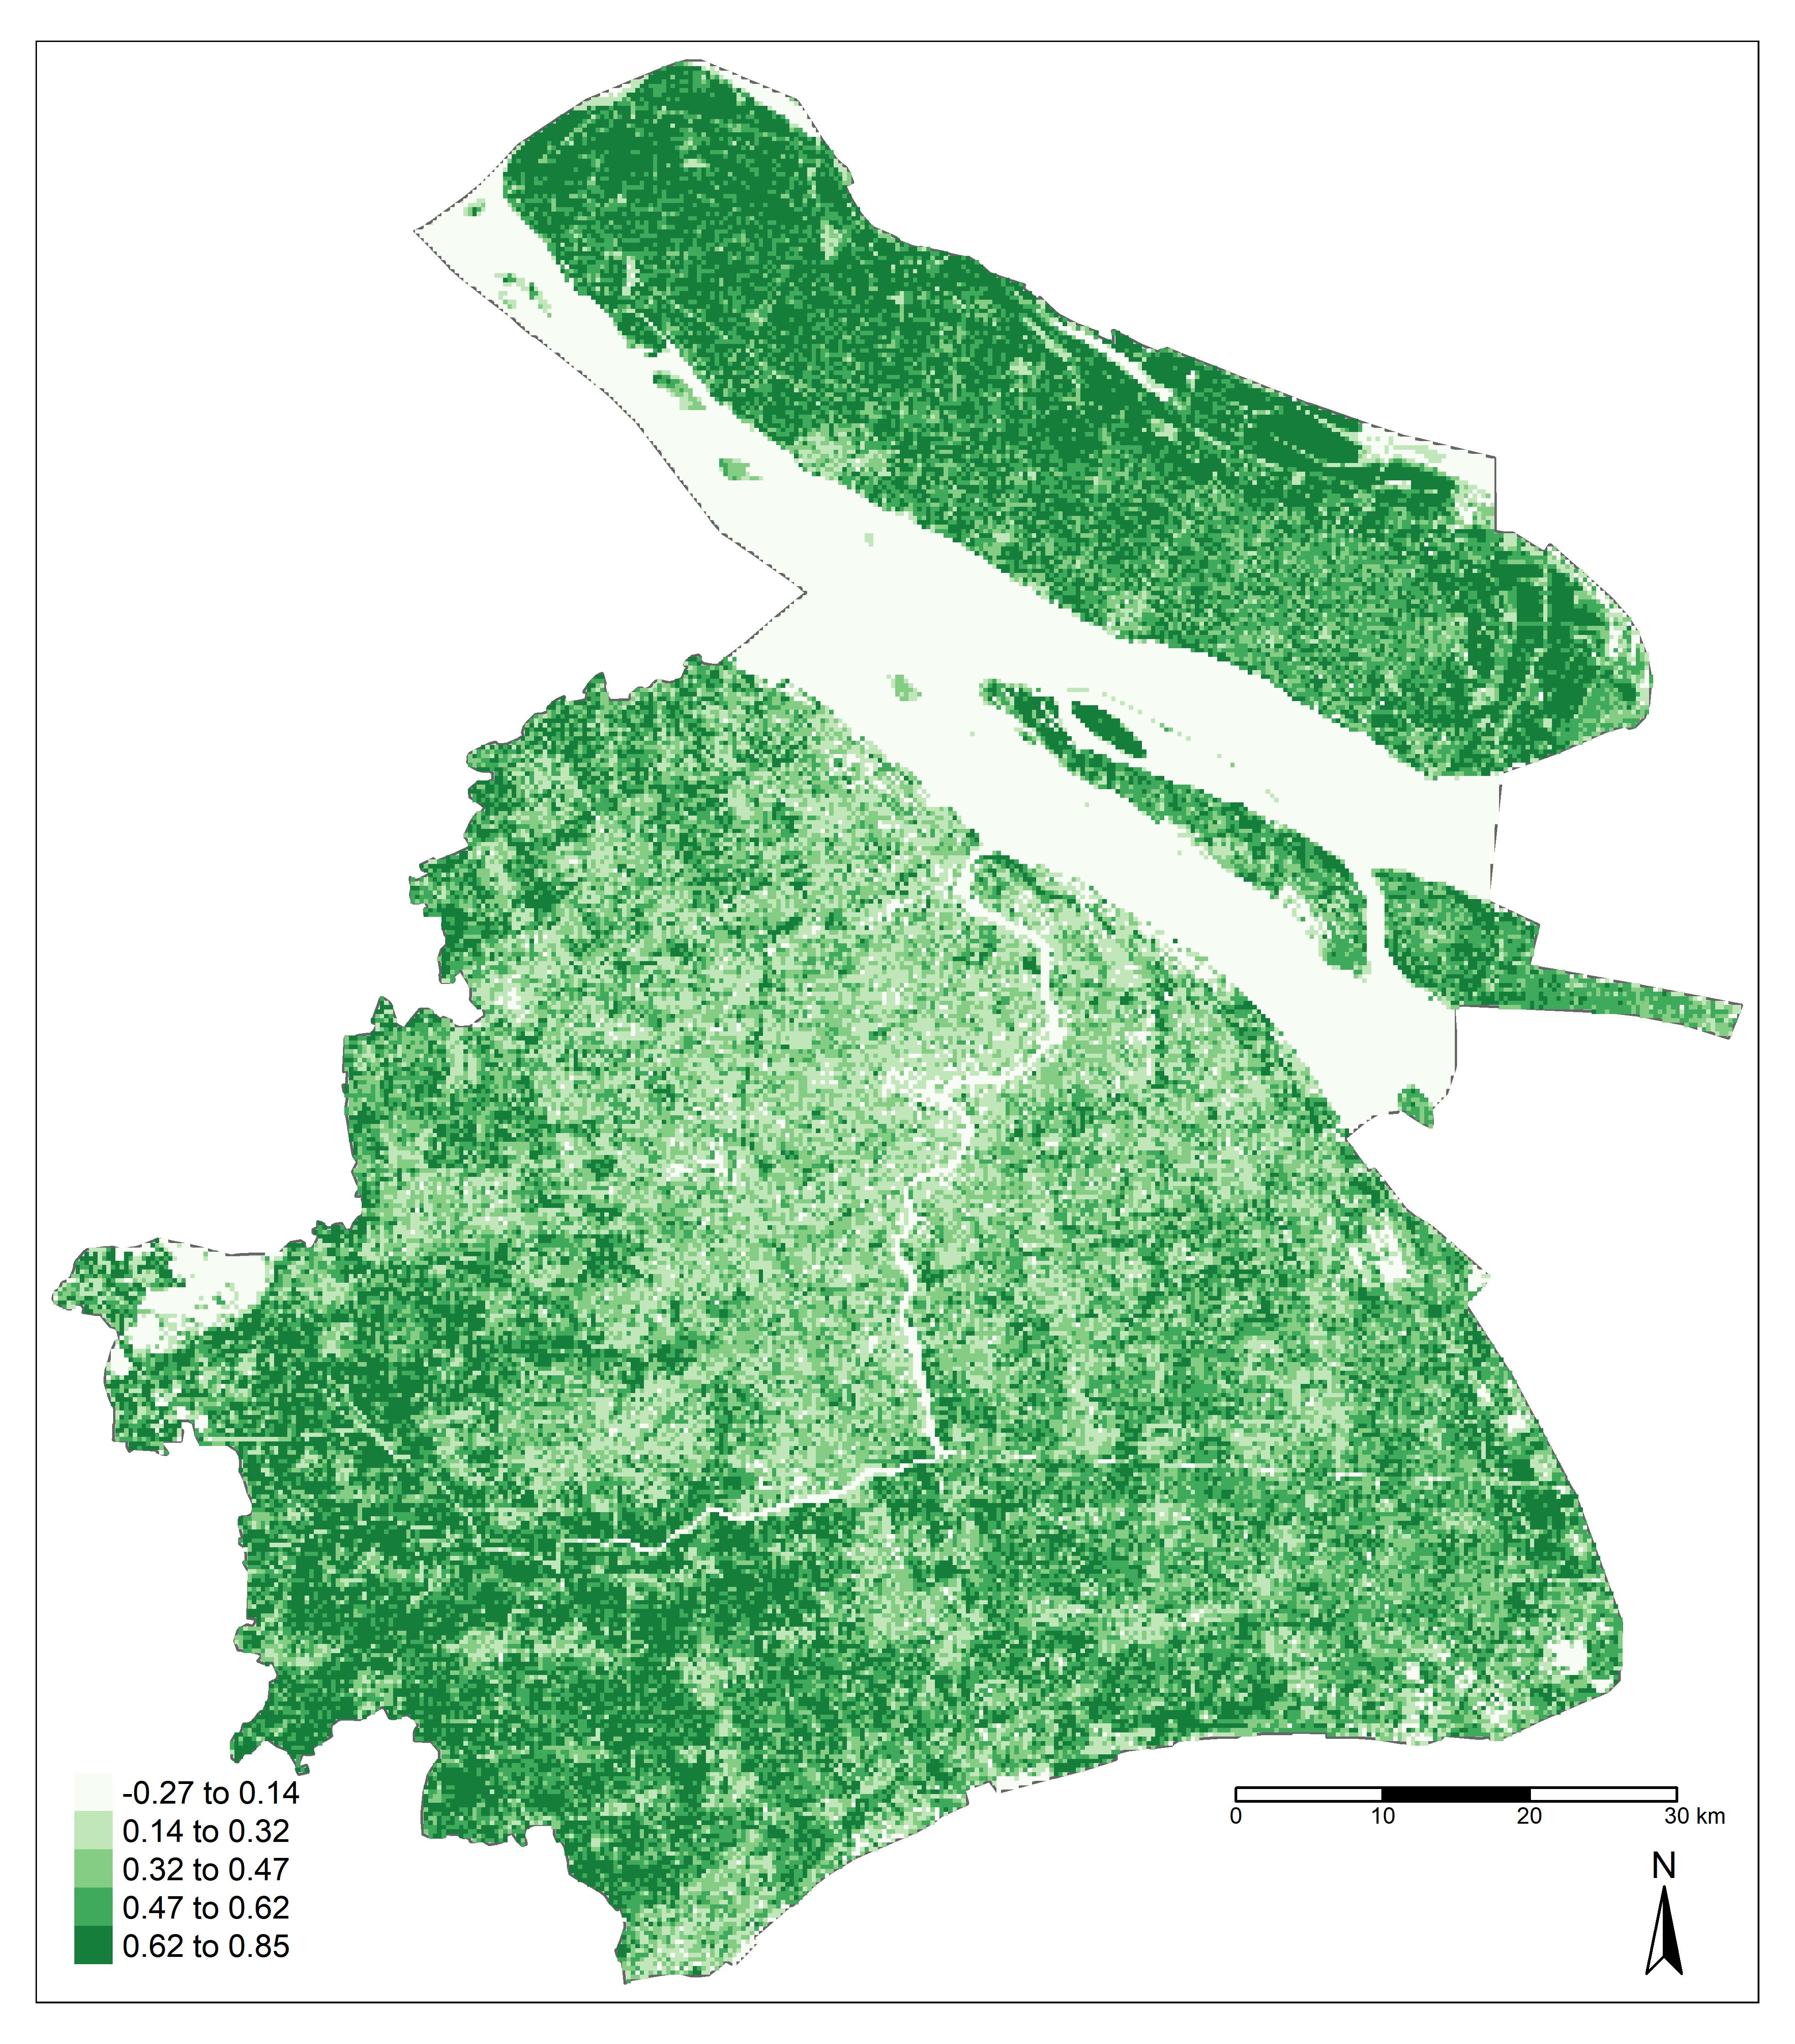
\includegraphics[width=6cm]{Figure/ndvi_sh.jpg}
}
\quad
\subfigure[NPP]{
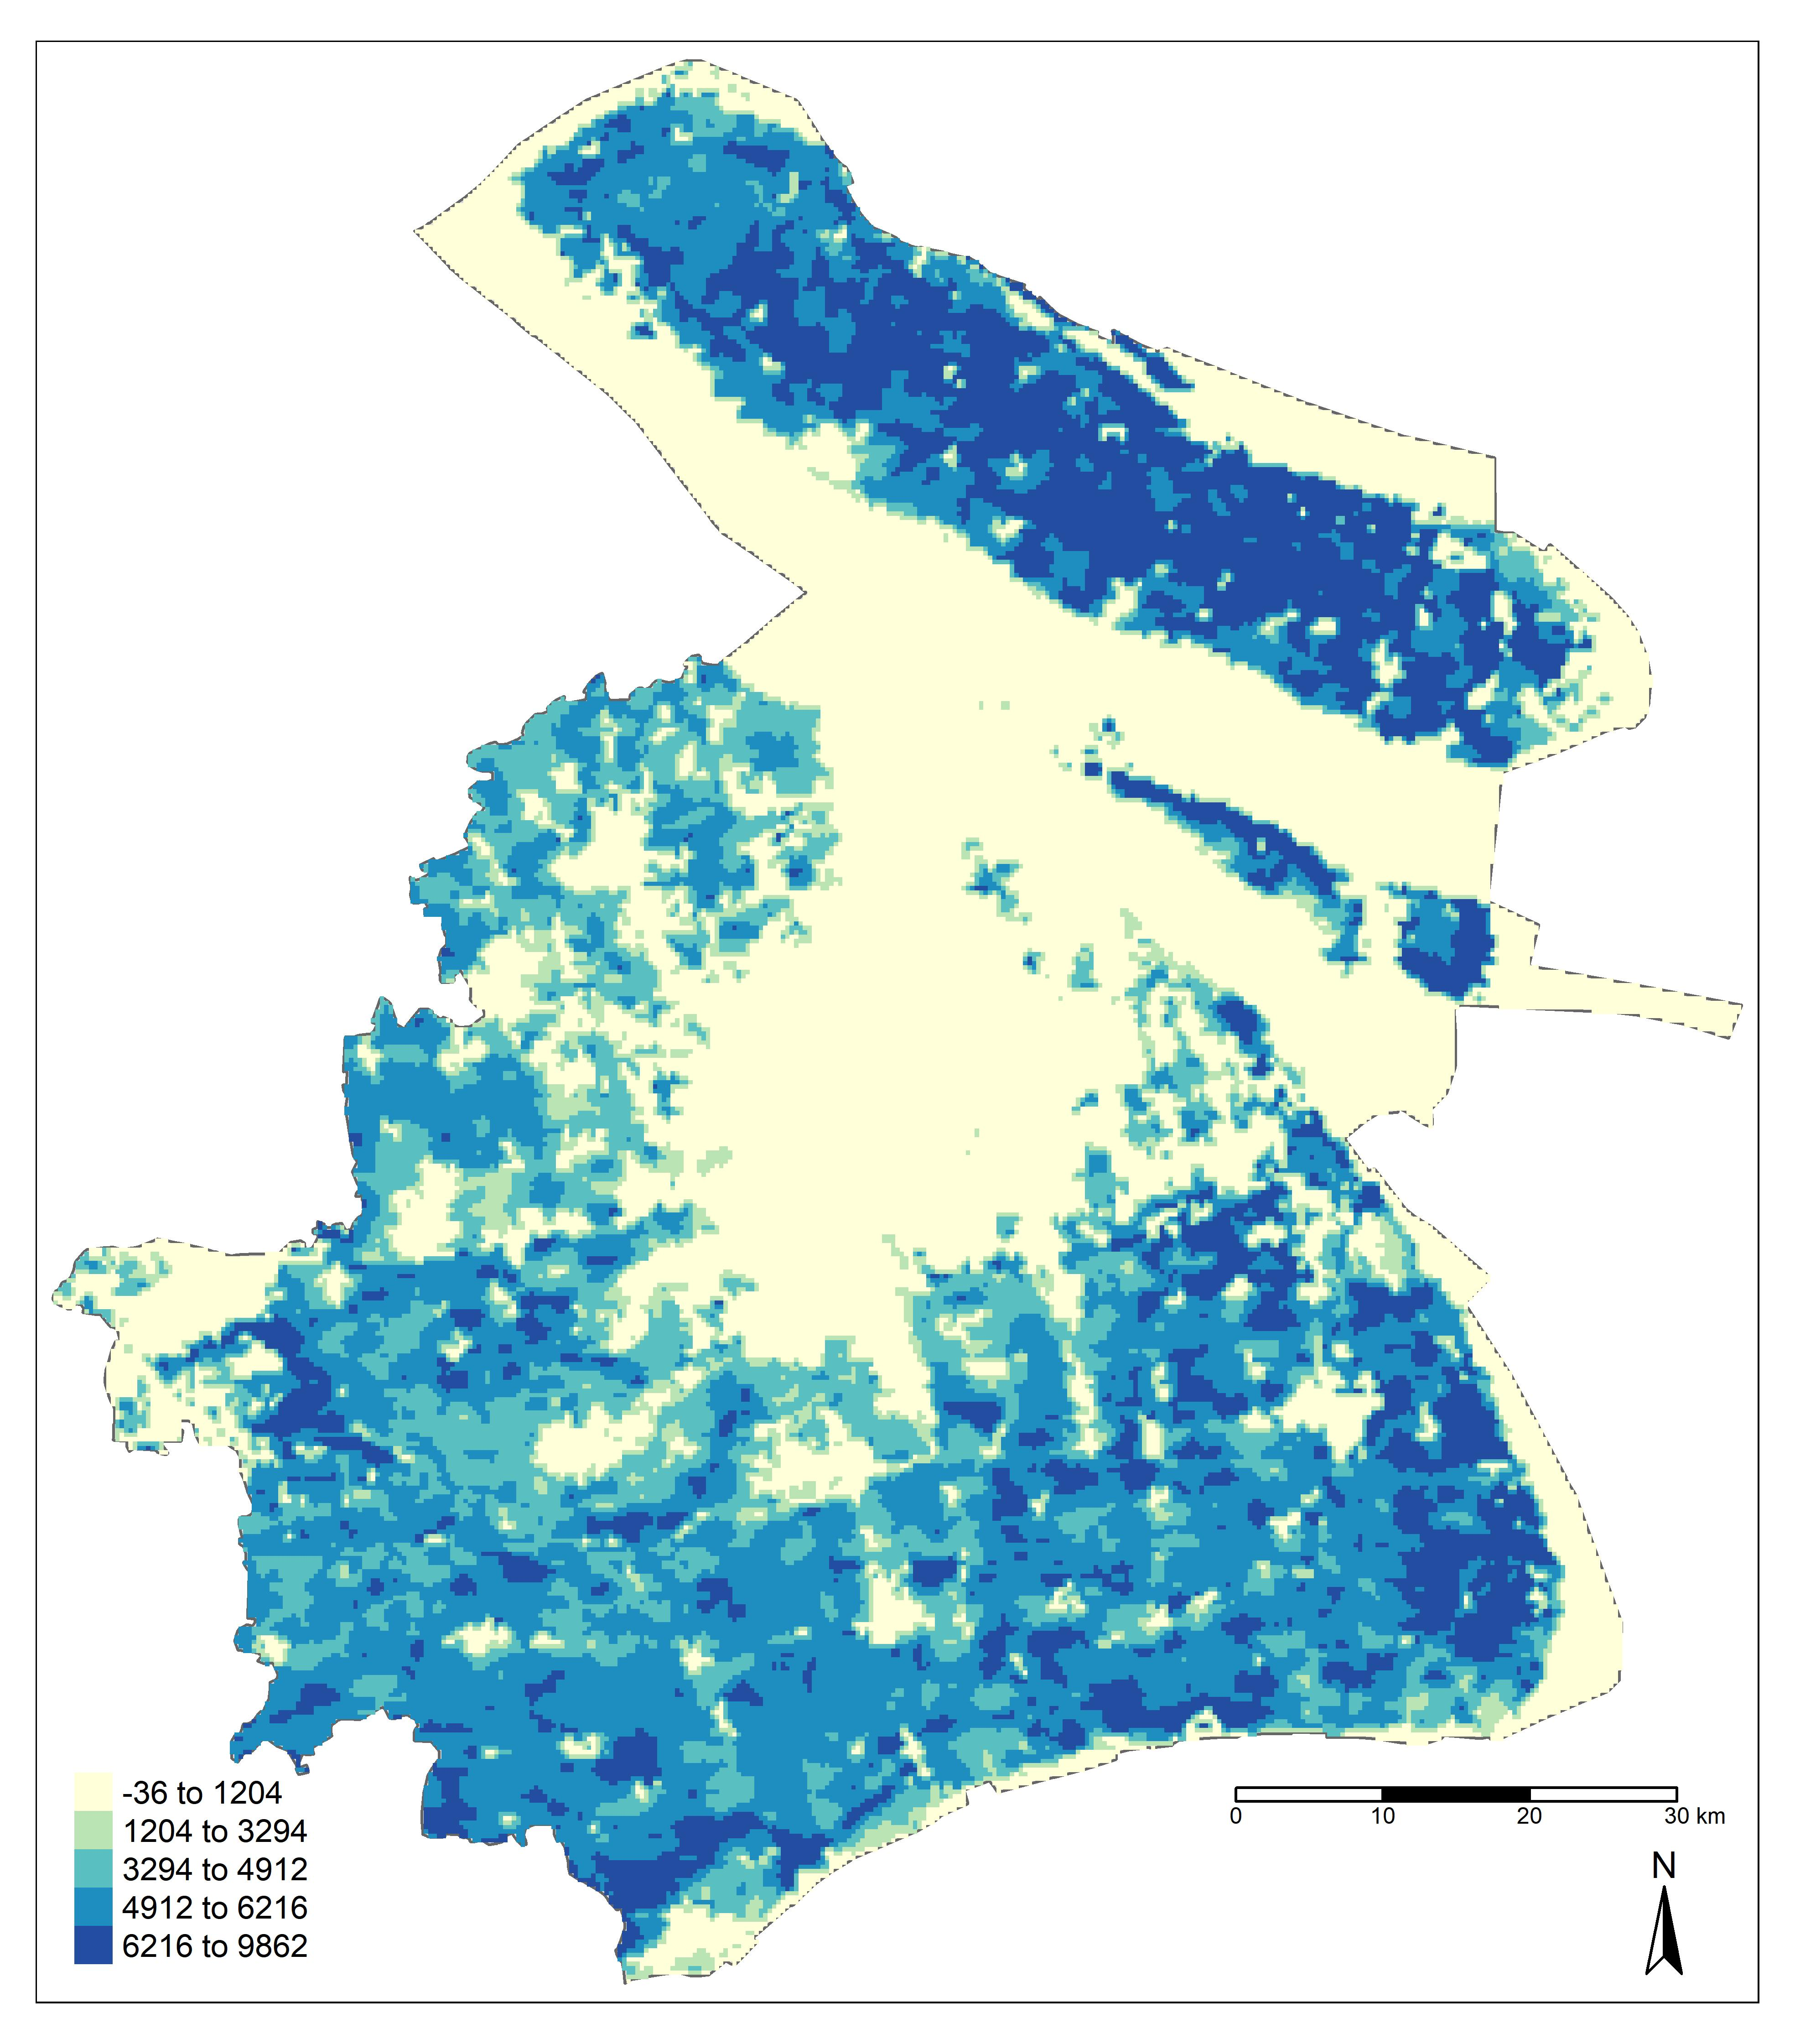
\includegraphics[width=6cm]{Figure/npp_sh.jpg}
}
\quad
\subfigure[PM2.5]{
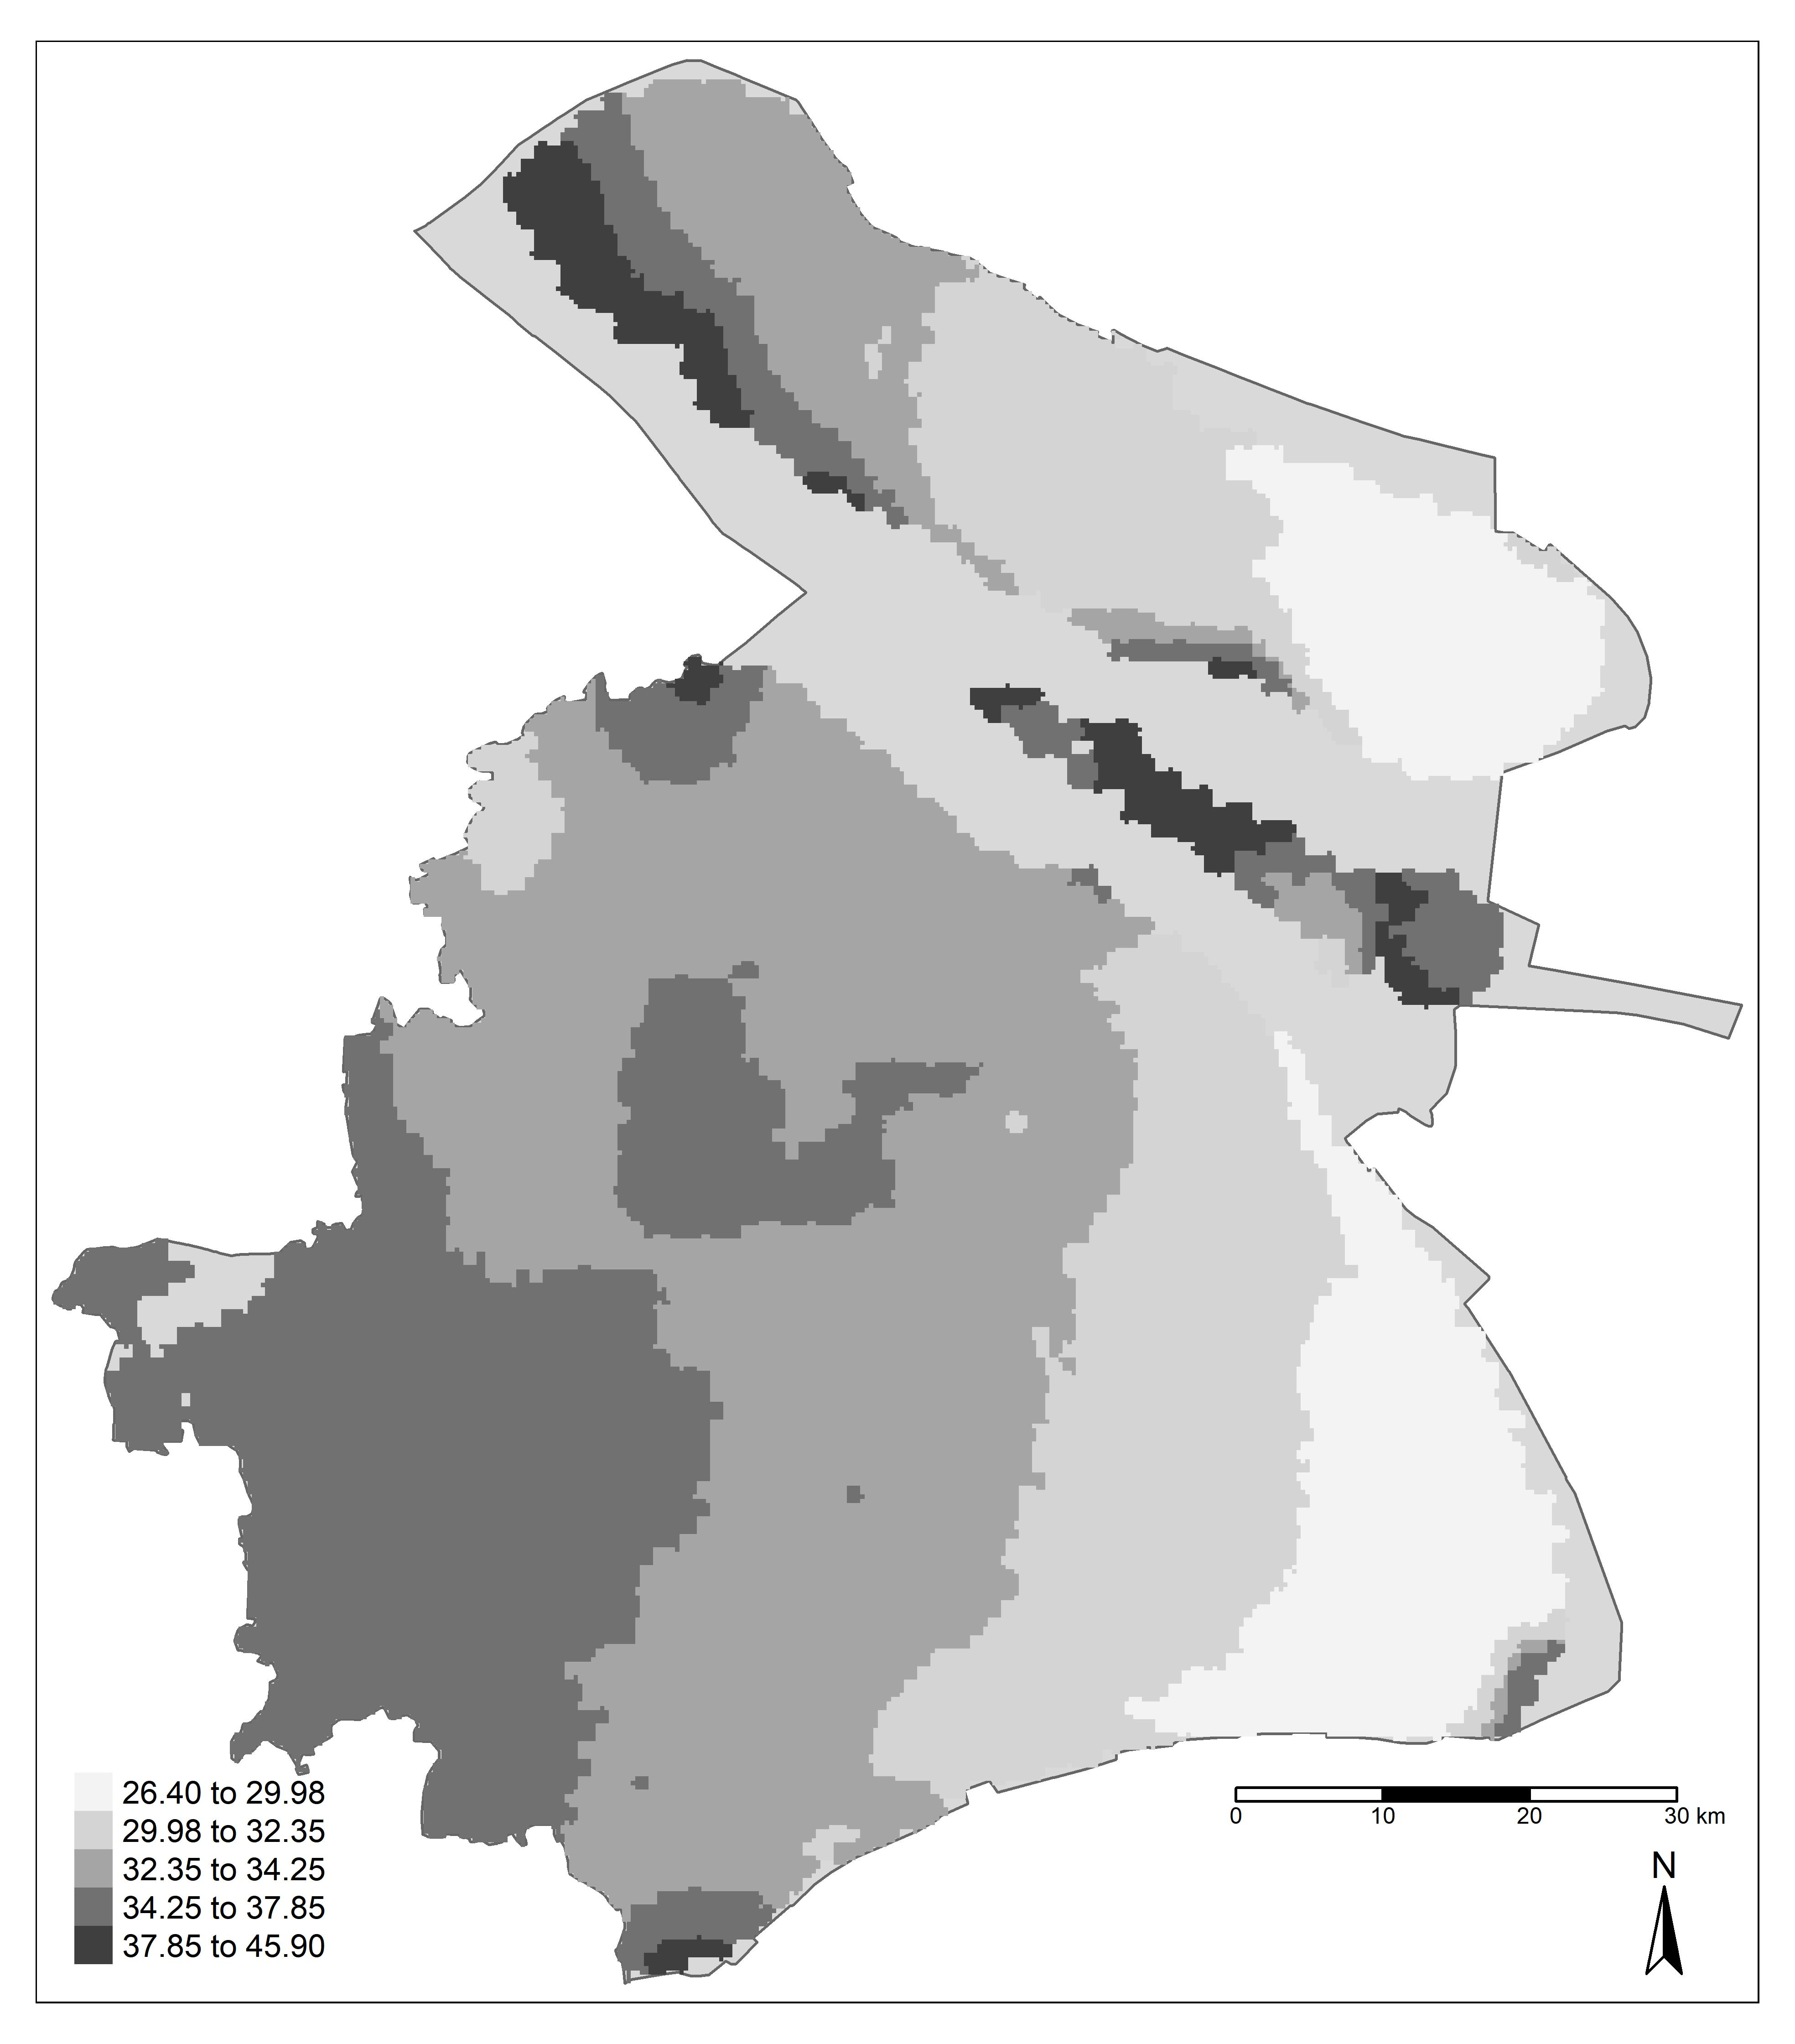
\includegraphics[width=6cm]{Figure/pm_sh.jpg}
}
\caption{Indicators of environmental system in Shanghai}
\label{esh}
\end{figure}
%%%%%%%%%%%%%%%%%%%%%%%%%%%%%%%%%%%%

\subsubsection{Environmental system indicators}
There were similarities in the spatial distribution of NPP and NDVI. The spatial layout of NDVI in Guangzhou showed a “moderately dense-sparse-dense” pattern from south to north area of the city. Shanghai city, on the other hand, showed a “dense-sparse-dense” pattern. By observing the two case cities, it can be seen that the high-value areas were concentrated around the central part of the cities. Different from NDVI, NPP was generally low or even zero in the construction land, which was due to the fact that impermeable surfaces could not perform the function of carbon fixation and oxygen emission.\\

When it comes to air quality indicator, PM25 has a significant difference from the other two environmental indicators. The high concentration areas in Guangzhou were distributed in the eastern and western parts of the city. The concentration of particulates gradually increased from the south to the central part of the city and decreased from the central part to the northern part of the city and finally dropped to the lowest value. By observation, it can be found that the PM25 concentration was the lowest in the northern woodland area, and the coastal area was also relatively low.\\

While in Shanghai, PM25 concentrations gradually show a trend from high to low from southwest to northeast. The PM25 concentration also becomes gradually lower in the area near the East China Sea.\\


\subsection{Comparation of urban fringe area in time series}
As shown in Figure \ref{totaldevelop}, the figure shows the changes of urban development index and environmental index in two cities from Guangzhou and Shanghai from 2013 to 2019 in the total area. The overall growth trend showed that both cities have been growing year by year in terms of urban development and environmental index.\\

The urban development index of Guangzhou has increased from 0.19 to 0.21 from 2013 to 2019, with a total increase of 1.11 times in these years. And the environmental index increased from 0.54 to 0.65 from 2013 to 2019, a total increase of 1.19 times.\\

%%%%%%%%%%%%%%%%%%%%%%%%%%%%%%%%%%%%
\begin{figure}[H]
\centering
\subfigure[Urban development system]{
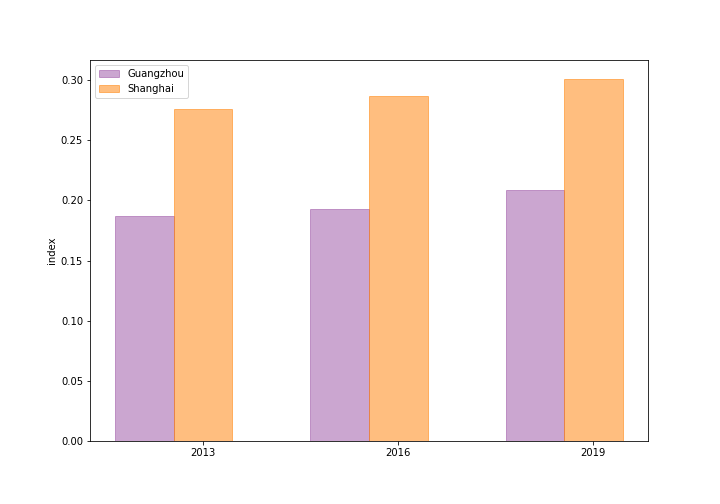
\includegraphics[width=6.5cm]{Figure/development_ur.png}
}
\quad
\subfigure[Environmental system]{
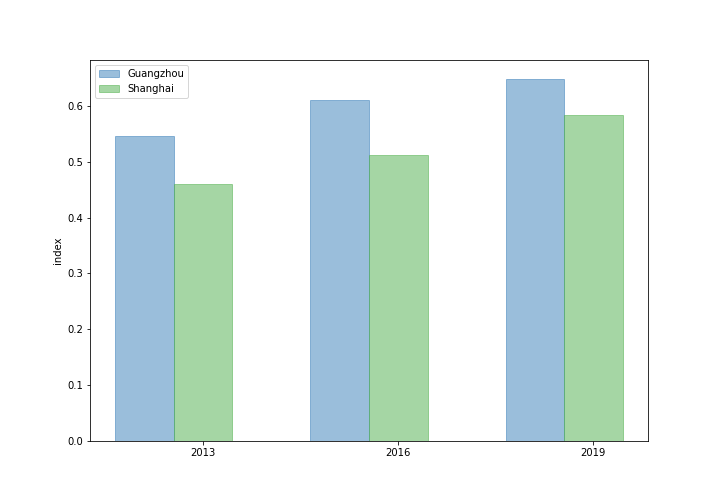
\includegraphics[width=6.5cm]{Figure/development_en.png}
}

\caption{The change of two system in total area from 2013 to 2019}
\label{totaldevelop}
\end{figure}
%%%%%%%%%%%%%%%%%%%%%%%%%%%%%%%%%%%%

On the contrary, Shanghai's urban development index increased from 0.27 to 0.30 from 2013 to 2019, a total increase of 1.09 times. And environmental index increased from 0.46 to 0.58 from 2013 to 2019, a total increase of 1.27 times.\\

It is obvious that Shanghai could have a significantly higher level of development than Guangzhou in the overall urban development index, while Guangzhou had an advantage in the environmental index compared to Shanghai. However, in terms of growth rate from 2013 to 2019, Guangzhou had a faster growth rate than Shanghai in terms of urban development, but slower than Shanghai in terms of environmental development.\\

When it comes to the change of two indicators in urban fringe area in Figure \ref{zonaldevelop}. The urban development index of Shanghai was still higher than that of Guangzhou in the urban fringe area unlike the total area, but the difference between the two cities was not significant. This would further prove that the identification of urban fringe area could effectively identify the urban fringe area. The urban development index of Guangzhou has increased from 0.33 to 0.36, with a total increase of 1.11 times. The urban development index of Shanghai increases from 0.34 to 0.36, with a total increase of 1.09 times.\\

%%%%%%%%%%%%%%%%%%%%%%%%%%%%%%%%%%%%
\begin{figure}[H]
\centering
\subfigure[Urban development system]{
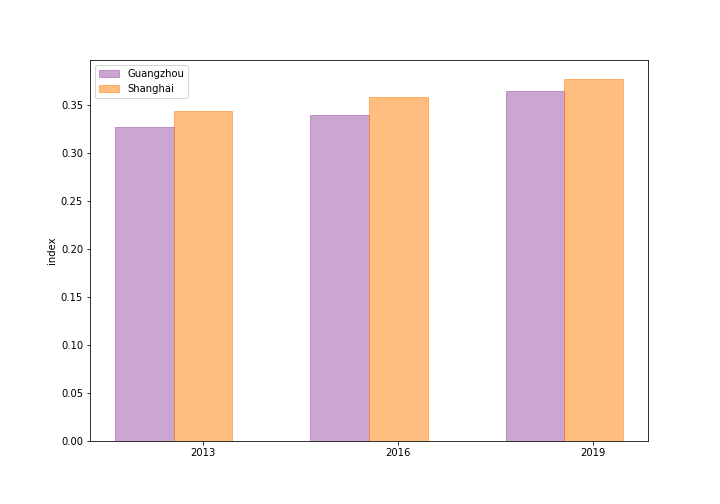
\includegraphics[width=6.5cm]{Figure/development_ur2.png}
}
\quad
\subfigure[Environmental system]{
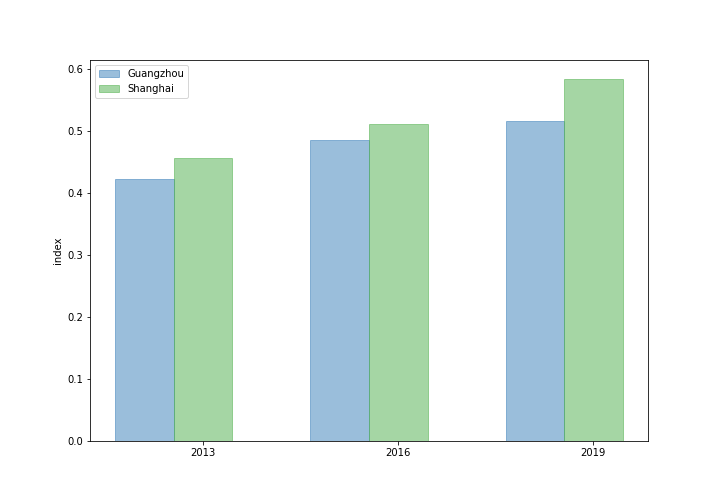
\includegraphics[width=6.5cm]{Figure/development_en2.png}
}

\caption{The change of two system in urban fringe area from 2013 to 2019}
\label{zonaldevelop}
\end{figure}
%%%%%%%%%%%%%%%%%%%%%%%%%%%%%%%%%%%%

At the same time, unlike the total area, Shanghai would have a higher environmental index than Guangzhou in the urban fringe area. The environmental index of Guangzhou increased from 0.42 to 0.51 by a total increasing ratio of 1.22. The environmental index of Shanghai increased from 0.46 to 0.58 by a total increasing ratio of 1.28. It is worth mentioning that the environmental index of Shanghai increased more from 2016 to 2019.\\

When focusing on the 3 indicators in urban development system (Figure \ref{ratiourban}), the study showed that the growth rate of the 3 indicators in both cities was always greater than 1 from 2013 to 2019. This also indicated that the level of urban construction was always in a state of development. However, the graph showed that the growth rate of AL and CL has slowed down from 2016 to 2019. This would also demonstrate that the rate of urban expansion was decreasing. In contrast to this, the growth rate of NT increased significantly from 2016 to 2019, which would also means that the overall level of urban land use was gradually increasing.\\

%%%%%%%%%%%%%%%%%%%%%%%%%%%%%%%%%%%%
\begin{figure}[H]
\centering
\subfigure[Guangzhou]{
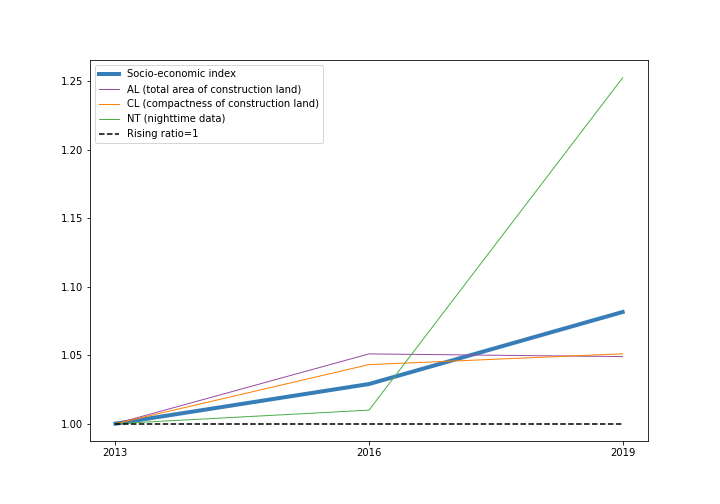
\includegraphics[width=6.5cm]{Figure/urbangz20821.png}
}
\quad
\subfigure[Shanghai]{
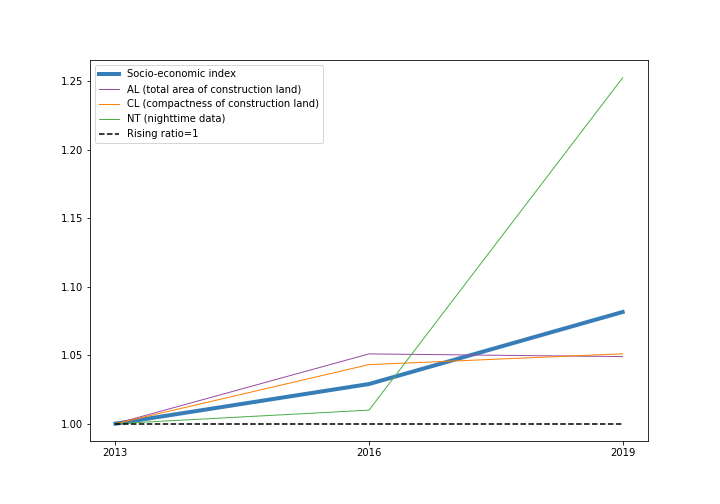
\includegraphics[width=6.5cm]{Figure/urbansh20821.png}
}

\caption{The raising ratio of urban development system from 2013 to 2019}
\label{ratiourban}
\end{figure}
%%%%%%%%%%%%%%%%%%%%%%%%%%%%%%%%%%%%

When it comes to 3 indicators in the environmental system (Figure \ref{ratioenvir}), the PM2.5 growth rate in both cities has been substantially less than 1 from 2013 to 2019, which would prove that air pollution was being gradually addressed. In Guangzhou, the NDVI value has been stable for six years, while the NPP has increased 1.13 times from 2016 to 2019. This could also prove that the level of carbon fixation and oxygen emission in Guangzhou has been improved. In contrast, the decline of NDVI and NPP in Shanghai was gradually increasing, which would be also further evidence that the ecological space was gradually being damaged while the city was developing. This is also something that needs more attention for future development.\\

%%%%%%%%%%%%%%%%%%%%%%%%%%%%%%%%%%%%
\begin{figure}[H]
\centering
\subfigure[Guangzhou]{
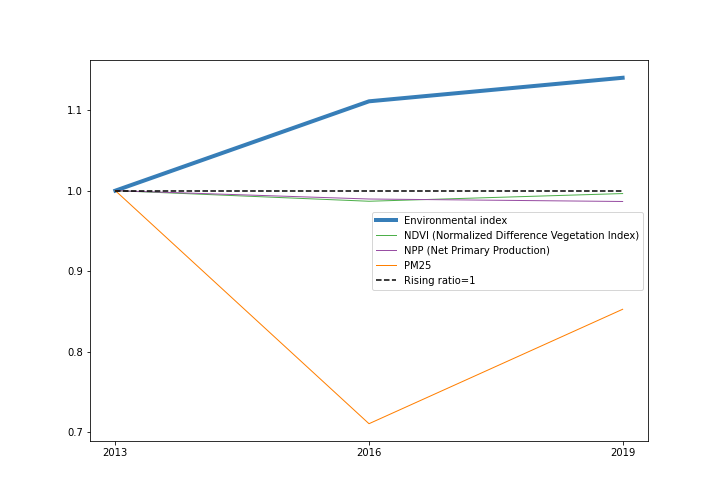
\includegraphics[width=6.5cm]{Figure/envirgz20821.png}
}
\quad
\subfigure[Shanghai]{
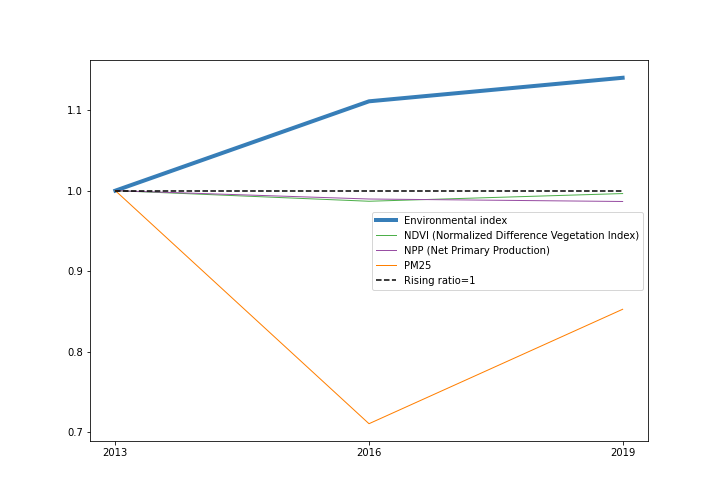
\includegraphics[width=6.5cm]{Figure/envirsh20821.png}
}

\caption{The raising ratio of environmental system from 2013 to 2019}
\label{ratioenvir}
\end{figure}
%%%%%%%%%%%%%%%%%%%%%%%%%%%%%%%%%%%%

\newpage
\section{Discussion}

\subsection{Research Implications}
This study provides a method for quantitative evaluation of fringe areas. This k-means clustering and edge detection method could allow the identification of cities area and bulk analysis of each urban fringe area.\\

The study can also discover urban development trends by using quantitative analysis of urban expansion mode in the past 9 years. In the process of studying data trends, the research would review relevant policies, urban development, and green space spatial planning policies over the years, which can search for effective evaluation of policy strengths and weaknesses. It can also Identify relevant problems with specific indicators and provide recommendations for future development policy.\\

Besides, through two case study cities (Guangzhou and Shanghai), the study could explore the development trend of a megacity in developing countries, especially in China. Specifically, there are advantages of economic urban development in coastal cities. Its ecological environment will also have considerable ecological advantages due to its water yield and other ecosystem services. At the same time, the coastal factor also has the necessary conditions to promote economic development by trade ports. \\

It is during this time that Guangzhou and Shanghai have been developed effectively. According to Guangzhou spatial planning (2020-2035) and Shanghai master planning (2020-2035), the development of the industrial development belts along the river has been consciously promoted. Guangzhou is planned to set a sub-center in the southern part of the city near the South China Sea. It has also consciously set the goal of building an international shipping hub to improve the function of international commerce. Shanghai, on the other hand, is planning to develop a new port area in the southeastern part of the city near the West China Sea. These planned areas are both located within the urban fringe. \\

Taking Guangzhou as an example, the strategy for the protection and management of the green space system in the spatial plan has been proposed to improve the environmental level of the northern area, optimize the quality of the central green space and increase the ecological space in the south area. Many scholars have to consider how much ecological green space should be added to the southern part of the city while considering the current situation of developing port trade.\\

By observing the fluctuation of ecological space and urban development space in urban fringe area, the study can effectively discover whether the environmental outcome of urban fringe area has increased or decreased within the suitable interval in the past years. Thus, it can effectively support the city planner in planning the ecological space and provide a reference for how much ecological space needs to be increased in the southern part of Guangzhou, for example. It also helps the megacities policymakers to quantify whether to protect all aspects of green space in the region when formulating development policies. This also helps them to coordinate ecological resources such as rivers, woodlands, and farmlands.\\



\subsection{Exploration of area changes}
\subsubsection{Socio-economic development: from expansion to contraction}
Through the result of 3 urban development indicators from urban fringe area in Guangzhou and Shanghai, the study found that the general growth rate of CL and AL have been decreasing, while the growth rate of NT has increased sharply in the last three years. It could be seen in general that the level of urban development has raised but the rate of expansion of urban area has decreased. It could be due to the fact that the urban area has gradually changed to be concentrated. Research shows that the aggregation of existing constructed land resources for urban development, which could successfully avoid the inefficient use of land \parencite{wang_dynamics_2020}. Overall, this development trend is positive. The change in CL and AL growth rates indicated that urban sprawl was gradually being halted. What’s more, the development pattern of the city in the last three years has also started to develop into an increase in commercial vitality and facilities within the built-up land. This could be also reflected in the significant increase in NT values over a nine-year period.\\

The development strategy(Shanghai City Master Plan (2020–2035)) has slowly changed from an urban sprawl-based development to an optimized land and space mode. For example, Guangzhou has removed the growth target of construction land from the plan and proposed a 15-minute walking distance concept. It also improved the public service facilities and built community centers to complete the spatial gathering in commercial facilities and population.\\

Nevertheless, the rate of urban constructed land conversion in the urban fringe remains at a high level and the concentration of urban area remains low. The data in the urban fringe area in the result shows that the development of urban fringe area was still driven by the expansion of building land. Despite reasonable planning under existing policies, sustainable development progress remains slow. Therefore, it is important to continue to optimize the direction of urban development by using additional strategies.\\


\subsubsection{Environmental outcome: decreasing ecosystem and optimizing air quality}
Surprisingly, it could be found through result that the environmental index has been increasing in the urban fringe area from 2013 to 2019. When the study is refined to the changes of 3 indicators in environmental system, we could clearly see the decrease in the overall rate of ecological degradation(NPP and NDVI). It could also prove that ecosystem service remained on an overall downward trend over the nine years. \\

With the guidance of the green space policy, megacities are doing their best to protect the ecological environment while developing the socio-economic status. Following the planning outline of ecological civilization construction in Guangzhou(2016-2020), Guangzhou could well regulate the air quality and ecological environment supported by the surrounding ecological resources to improve the current situation.\\

The strategy of greening the environment was effective, but it was still difficult to contain the ecological changes in the fringe area. The overall quality of air quality has increased. It was the improvement in air quality that effectively saw the overall environmental index rise over a 9-year period. It showed that cities were making progress on carbon emission policies and were able to optimize air quality. According to Shanghai City Master Plan (2020–2035), the planning strategies were going to create a high-level low carbon island concept in the northern islands of the region. However, the local low-carbon policy attempts were still not effective in improving the urban fringe area, and it may be necessary to implement low-carbon policies on a smaller scale in more areas.\\

However, when it comes to the difference between fringe area and urban area, the rate of air quality optimization was still lower than in the urban area, especially in Guangzhou. In the urban fringe area in the east and west of Guangzhou area, the PM2.5 concentration was still the highest. And the degree of change in this region has remained in the state of slow change in 9 years.\\

It could probably be due to the construction of industrial areas in the urban fringe on the one hand, and the shift of industries in the urban area on the other hand, which can lead to an industrial structural disadvantage in terms of air quality in the urban fringe area.\\



\subsection{Future optimization and restoration from the research: urban land use consolidation and ecological protection}
By comparing urban development system and environmental system in two cities, the study shows that urban development patterns still exist in the area with the cost of the ecological environment, especially in ecosystem services including carbon and water resource. With their relatively limited ecological resources, Guangzhou and Shanghai still need intensive ecological conservation in the direction of conservation. Therefore, optimization and restoration strategies in the urban fringe area should be purposed when facing this problem. \\

Two case study cities have carried out a series of projects and plans such as ecological protection redline, however, these “bottom-line” policies mainly concerned ecological space while neglecting the human-land contradiction in urban fringe area \parencite{xu_developing_2021}. An inefficient construction land reduction plan and land levelling plan were also purposed by city planners in the Master plan from Shanghai. However, the plan still has no specific unified implementation strategy \parencite{sun_road_2021}.\\

The study would propose some methods for land use consolidation and ecological protection according to the result from two case study cities. When it comes to urban development system in urban fringe area, the land use consolidation method should be implemented. For example, fragments patches should be Integrated through land consolidation, which can integrate different spaces with various kinds of land-use area in a unified way \parencite{bush_building_2019}. It can be carried out spatial reconfiguration in the planning process in the district area. Since the planning of land functions would take the district as the planning unit, the district planning should start from a centralized planning approach, which means that the construction land should be unified into one community in planning.\\

Ecological restoration in urban fringe area should be a conservation and restoration priority. For example, constructed land in the urban fringe area could be improved by combining green and blue spaces to form an ecological network and green infrastructure \parencite{yu_critical_2020}. Small green spaces could be constructed and distributed throughout constructed land to maintain the steady of ecosystem. Among them, in Shanghai short-term territorial spatial planning (2020-2025), urban planners have made a preliminary plan for the short-term ecological pattern of 'one green ring, 3 ecological corridors and 4 ecological park areas'. Where the green ring was to be built around the urban construction area in the central part of the city. And the plan has established two ecological corridors in the area of the urban fringe in the south of the city. This ecological corridor was connected with green areas along the road. The ecological corridors could be restored and constructed by the environmental outcome of this study. The specific way of restoration could be in the form of small green space. On the other hand, ecological restoration in urban fringe area could also improve by enriching the urban fringe corridors with various types, vegetation species and vertical structures\parencite{yang_construction_2018}.\\


\subsection{Limitation and challenge}
Due to the limited time of the dataset, there is no way to analyze the study in more depth from a 10 year to 20 year perspective. According to some research, factors such as road traffic could be considered in the identification of urban fringe areas. Therefore, more influential factors need to be taken into account in future studies.\\

On the other hand, due to the small variation in some of the indicators, there could be no way to effectively quantify the valid results of the indicator. In the future, a selection of case cities in different policy contexts (protection of development priority) could be considered for more in-depth analysis.\\
 

\newpage
\section{Conclusion}
Urban construction and socio-economic development remain the dominant theme of development in developing countries as well as all over the world. However, when it comes to the context of climate change and urban sprawl, the question of how to develop the city sustainably in the face of unrestricted urban growth and population expansion is something that needs to be deeply discussed by a wide range of scholars. The urban fringe area is the most prominent area for urbanization-related social-ecological problems. The urban fringe area is the most prominent area for urbanization-related social-ecological problems. As the most mature area of urbanization, megacities should develop this area through a well-coordinated and balanced approach.\\

The study explored the trends of urban development system and environmental system in urban fringe area through two case cities in China, Guangzhou and Shanghai, and tries to find the balance point between the two systems.\\

Specifically, the study identified the urban fringe area in two cities by K-means clustering analysis. The study also investigated the relationship between urban fringe area and total area and compared the urban fringe area with the trend of urban development and ecological changes in the past 9 years to explore the effectiveness of the fringe area under the current policies.\\

Through K-means analysis, the study effectively identified urban area, urban fringe area and suburban area. Compared with other areas, the urban fringe area has changed more significantly in urban development system and environmental system in 9 years. Besides, the land use type of this area had become more fragmented.\\

The data analysis of urban fringe area in the two cities shows that urban development index and environmental index of Guangzhou and Shanghai have been on an increasing trend from 2013 to 2019. The urban sprawl has gradually slowed down, and the urban strategy has gradually changed from external expansion to internal spatial optimization. In terms of environment, the air quality of Urban fringe area has improved significantly, but ecosystem services such as carbon fixation still show a decline in general.\\

In response to the result, the study tried to propose a development strategy for urban fringe area with the integration of land-intensive development and ecological restoration. The study also explored the method to integrate the scattered construction land into a uniform large-scale patch in the actual planning and construction process and convert the useless and low-value construction land into ecological space. By doing this, the level of urban development could be improved. In addition, ecological restoration strategies such as increasing scattered green space and optimizing ecological corridors could be used to protect and utilize ecology. \\

This study aims to help megacities to evaluate urban fringe area policies by proposing a unified and convenient method for identifying urban fringe area. Besides, it can also quantify the socio-economic and environmental evaluation of urban fringe area. The project helps policymakers to evaluate the policies of urban fringe area. It will provide a reference for megacities' development model in sustainable policies.\\
 

% -------------------  BIBLIOGRAPHY ---------------------
\newpage
\printbibliography[title = {References}]
\addcontentsline{toc}{chapter}{References} % Adds References Section to Table of Contents


\end{document}
%  -------------------------------------------------
%  --------- The document ends from here ----------- 
%  -------------------------------------------------